\documentclass[]{book}
\usepackage{lmodern}
\usepackage{amssymb,amsmath}
\usepackage{ifxetex,ifluatex}
\usepackage{fixltx2e} % provides \textsubscript
\ifnum 0\ifxetex 1\fi\ifluatex 1\fi=0 % if pdftex
  \usepackage[T1]{fontenc}
  \usepackage[utf8]{inputenc}
\else % if luatex or xelatex
  \ifxetex
    \usepackage{mathspec}
  \else
    \usepackage{fontspec}
  \fi
  \defaultfontfeatures{Ligatures=TeX,Scale=MatchLowercase}
\fi
% use upquote if available, for straight quotes in verbatim environments
\IfFileExists{upquote.sty}{\usepackage{upquote}}{}
% use microtype if available
\IfFileExists{microtype.sty}{%
\usepackage{microtype}
\UseMicrotypeSet[protrusion]{basicmath} % disable protrusion for tt fonts
}{}
\usepackage[margin=1in]{geometry}
\usepackage{hyperref}
\hypersetup{unicode=true,
            pdftitle={A bookdown Example},
            pdfauthor={BPLIM staff},
            pdfborder={0 0 0},
            breaklinks=true}
\urlstyle{same}  % don't use monospace font for urls
\usepackage{natbib}
\bibliographystyle{apalike}
\usepackage{color}
\usepackage{fancyvrb}
\newcommand{\VerbBar}{|}
\newcommand{\VERB}{\Verb[commandchars=\\\{\}]}
\DefineVerbatimEnvironment{Highlighting}{Verbatim}{commandchars=\\\{\}}
% Add ',fontsize=\small' for more characters per line
\usepackage{framed}
\definecolor{shadecolor}{RGB}{248,248,248}
\newenvironment{Shaded}{\begin{snugshade}}{\end{snugshade}}
\newcommand{\AlertTok}[1]{\textcolor[rgb]{0.94,0.16,0.16}{#1}}
\newcommand{\AnnotationTok}[1]{\textcolor[rgb]{0.56,0.35,0.01}{\textbf{\textit{#1}}}}
\newcommand{\AttributeTok}[1]{\textcolor[rgb]{0.77,0.63,0.00}{#1}}
\newcommand{\BaseNTok}[1]{\textcolor[rgb]{0.00,0.00,0.81}{#1}}
\newcommand{\BuiltInTok}[1]{#1}
\newcommand{\CharTok}[1]{\textcolor[rgb]{0.31,0.60,0.02}{#1}}
\newcommand{\CommentTok}[1]{\textcolor[rgb]{0.56,0.35,0.01}{\textit{#1}}}
\newcommand{\CommentVarTok}[1]{\textcolor[rgb]{0.56,0.35,0.01}{\textbf{\textit{#1}}}}
\newcommand{\ConstantTok}[1]{\textcolor[rgb]{0.00,0.00,0.00}{#1}}
\newcommand{\ControlFlowTok}[1]{\textcolor[rgb]{0.13,0.29,0.53}{\textbf{#1}}}
\newcommand{\DataTypeTok}[1]{\textcolor[rgb]{0.13,0.29,0.53}{#1}}
\newcommand{\DecValTok}[1]{\textcolor[rgb]{0.00,0.00,0.81}{#1}}
\newcommand{\DocumentationTok}[1]{\textcolor[rgb]{0.56,0.35,0.01}{\textbf{\textit{#1}}}}
\newcommand{\ErrorTok}[1]{\textcolor[rgb]{0.64,0.00,0.00}{\textbf{#1}}}
\newcommand{\ExtensionTok}[1]{#1}
\newcommand{\FloatTok}[1]{\textcolor[rgb]{0.00,0.00,0.81}{#1}}
\newcommand{\FunctionTok}[1]{\textcolor[rgb]{0.00,0.00,0.00}{#1}}
\newcommand{\ImportTok}[1]{#1}
\newcommand{\InformationTok}[1]{\textcolor[rgb]{0.56,0.35,0.01}{\textbf{\textit{#1}}}}
\newcommand{\KeywordTok}[1]{\textcolor[rgb]{0.13,0.29,0.53}{\textbf{#1}}}
\newcommand{\NormalTok}[1]{#1}
\newcommand{\OperatorTok}[1]{\textcolor[rgb]{0.81,0.36,0.00}{\textbf{#1}}}
\newcommand{\OtherTok}[1]{\textcolor[rgb]{0.56,0.35,0.01}{#1}}
\newcommand{\PreprocessorTok}[1]{\textcolor[rgb]{0.56,0.35,0.01}{\textit{#1}}}
\newcommand{\RegionMarkerTok}[1]{#1}
\newcommand{\SpecialCharTok}[1]{\textcolor[rgb]{0.00,0.00,0.00}{#1}}
\newcommand{\SpecialStringTok}[1]{\textcolor[rgb]{0.31,0.60,0.02}{#1}}
\newcommand{\StringTok}[1]{\textcolor[rgb]{0.31,0.60,0.02}{#1}}
\newcommand{\VariableTok}[1]{\textcolor[rgb]{0.00,0.00,0.00}{#1}}
\newcommand{\VerbatimStringTok}[1]{\textcolor[rgb]{0.31,0.60,0.02}{#1}}
\newcommand{\WarningTok}[1]{\textcolor[rgb]{0.56,0.35,0.01}{\textbf{\textit{#1}}}}
\usepackage{longtable,booktabs}
\usepackage{graphicx,grffile}
\makeatletter
\def\maxwidth{\ifdim\Gin@nat@width>\linewidth\linewidth\else\Gin@nat@width\fi}
\def\maxheight{\ifdim\Gin@nat@height>\textheight\textheight\else\Gin@nat@height\fi}
\makeatother
% Scale images if necessary, so that they will not overflow the page
% margins by default, and it is still possible to overwrite the defaults
% using explicit options in \includegraphics[width, height, ...]{}
\setkeys{Gin}{width=\maxwidth,height=\maxheight,keepaspectratio}
\IfFileExists{parskip.sty}{%
\usepackage{parskip}
}{% else
\setlength{\parindent}{0pt}
\setlength{\parskip}{6pt plus 2pt minus 1pt}
}
\setlength{\emergencystretch}{3em}  % prevent overfull lines
\providecommand{\tightlist}{%
  \setlength{\itemsep}{0pt}\setlength{\parskip}{0pt}}
\setcounter{secnumdepth}{5}
% Redefines (sub)paragraphs to behave more like sections
\ifx\paragraph\undefined\else
\let\oldparagraph\paragraph
\renewcommand{\paragraph}[1]{\oldparagraph{#1}\mbox{}}
\fi
\ifx\subparagraph\undefined\else
\let\oldsubparagraph\subparagraph
\renewcommand{\subparagraph}[1]{\oldsubparagraph{#1}\mbox{}}
\fi

%%% Use protect on footnotes to avoid problems with footnotes in titles
\let\rmarkdownfootnote\footnote%
\def\footnote{\protect\rmarkdownfootnote}

%%% Change title format to be more compact
\usepackage{titling}

% Create subtitle command for use in maketitle
\providecommand{\subtitle}[1]{
  \posttitle{
    \begin{center}\large#1\end{center}
    }
}

\setlength{\droptitle}{-2em}

  \title{A bookdown Example}
    \pretitle{\vspace{\droptitle}\centering\huge}
  \posttitle{\par}
    \author{BPLIM staff}
    \preauthor{\centering\large\emph}
  \postauthor{\par}
      \predate{\centering\large\emph}
  \postdate{\par}
    \date{2019-05-27}

\usepackage{booktabs}
\usepackage{amsthm}
\usepackage{graphicx}
\makeatletter
\def\thm@space@setup{%
  \thm@preskip=8pt plus 2pt minus 4pt
  \thm@postskip=\thm@preskip
}
\makeatother

\begin{document}
\maketitle

{
\setcounter{tocdepth}{1}
\tableofcontents
}

\includegraphics[width=0.328\linewidth]{media/logo}

\hypertarget{prerequisites}{%
\chapter{Prerequisites}\label{prerequisites}}

This is a \emph{sample} book written in \textbf{Markdown}. You can use anything that Pandoc's Markdown supports, e.g., a math equation \(a^2 + b^2 = c^2\).\footnote{While\ldots{}}

\[\begin{array}{ccc}
x_{11} & x_{12} & x_{13}\\
x_{21} & x_{22} & x_{23}
\end{array}\]

The \textbf{bookdown} package can be installed from CRAN or Github:

\begin{Shaded}
\begin{Highlighting}[]
\KeywordTok{install.packages}\NormalTok{(}\StringTok{"bookdown"}\NormalTok{)}
\CommentTok{# or the development version}

\CommentTok{## devtools::install_github("rstudio/bookdown")}
\CommentTok{## bookdown::render_book("index.Rmd", "bookdown::epub_book")}
\CommentTok{## bookdown::render_book("index.Rmd", "bookdown::pdf_book")}
\CommentTok{## bookdown::render_book("index.Rmd", "all",new_session = TRUE)}
\end{Highlighting}
\end{Shaded}

Remember each Rmd file contains one and only one chapter, and a chapter is defined by the first-level heading \texttt{\#}.

To compile this example to PDF, you need XeLaTeX. You are recommended to install TinyTeX (which includes XeLaTeX): \url{https://yihui.name/tinytex/}.

\hypertarget{intro}{%
\chapter{Introduction}\label{intro}}

You can label chapter and section titles using \texttt{\{\#label\}} after them, e.g., we can reference Chapter \ref{intro}. If you do not manually label them, there will be automatic labels anyway, e.g., Chapter \ref{methods}.

Figures and tables with captions will be placed in \texttt{figure} and \texttt{table} environments, respectively.

\begin{figure}

{\centering 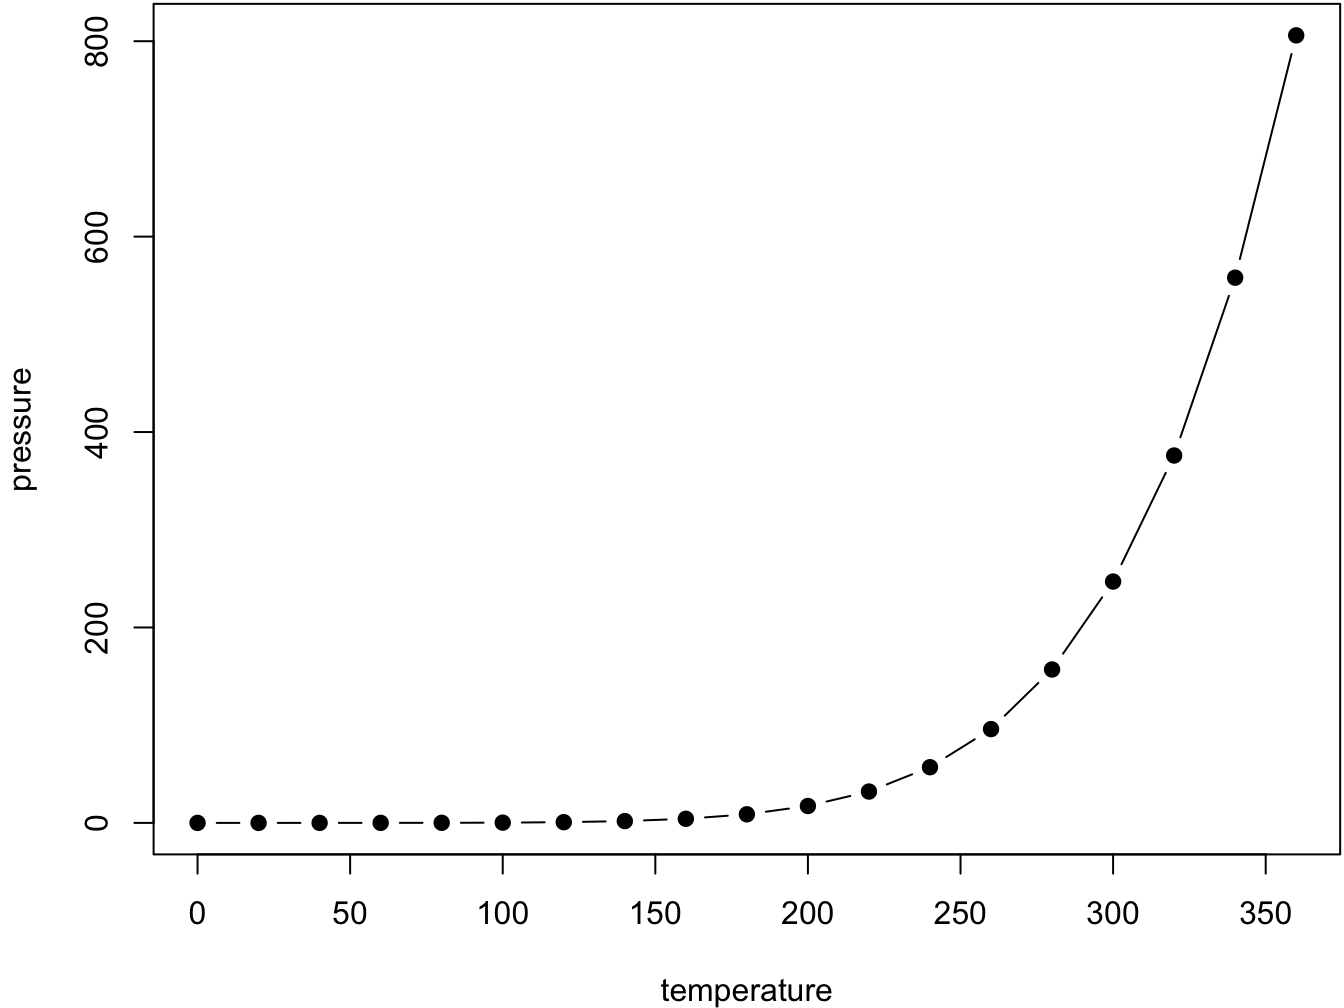
\includegraphics[width=0.8\linewidth]{bookdown-demo_files/figure-latex/nice-fig-1} 

}

\caption{Here is a nice figure!}\label{fig:nice-fig}
\end{figure}

Reference a figure by its code chunk label with the \texttt{fig:} prefix, e.g., see Figure \ref{fig:nice-fig}. Similarly, you can reference tables generated from \texttt{knitr::kable()}, e.g., see Table \ref{tab:nice-tab}.

\begin{Shaded}
\begin{Highlighting}[]
\NormalTok{knitr}\OperatorTok{::}\KeywordTok{kable}\NormalTok{(}
  \KeywordTok{head}\NormalTok{(iris, }\DecValTok{20}\NormalTok{), }\DataTypeTok{caption =} \StringTok{'Here is a nice table!'}\NormalTok{,}
  \DataTypeTok{booktabs =} \OtherTok{TRUE}
\NormalTok{)}
\end{Highlighting}
\end{Shaded}

\begin{table}[t]

\caption{\label{tab:nice-tab}Here is a nice table!}
\centering
\begin{tabular}{rrrrl}
\toprule
Sepal.Length & Sepal.Width & Petal.Length & Petal.Width & Species\\
\midrule
5.1 & 3.5 & 1.4 & 0.2 & setosa\\
4.9 & 3.0 & 1.4 & 0.2 & setosa\\
4.7 & 3.2 & 1.3 & 0.2 & setosa\\
4.6 & 3.1 & 1.5 & 0.2 & setosa\\
5.0 & 3.6 & 1.4 & 0.2 & setosa\\
\addlinespace
5.4 & 3.9 & 1.7 & 0.4 & setosa\\
4.6 & 3.4 & 1.4 & 0.3 & setosa\\
5.0 & 3.4 & 1.5 & 0.2 & setosa\\
4.4 & 2.9 & 1.4 & 0.2 & setosa\\
4.9 & 3.1 & 1.5 & 0.1 & setosa\\
\addlinespace
5.4 & 3.7 & 1.5 & 0.2 & setosa\\
4.8 & 3.4 & 1.6 & 0.2 & setosa\\
4.8 & 3.0 & 1.4 & 0.1 & setosa\\
4.3 & 3.0 & 1.1 & 0.1 & setosa\\
5.8 & 4.0 & 1.2 & 0.2 & setosa\\
\addlinespace
5.7 & 4.4 & 1.5 & 0.4 & setosa\\
5.4 & 3.9 & 1.3 & 0.4 & setosa\\
5.1 & 3.5 & 1.4 & 0.3 & setosa\\
5.7 & 3.8 & 1.7 & 0.3 & setosa\\
5.1 & 3.8 & 1.5 & 0.3 & setosa\\
\bottomrule
\end{tabular}
\end{table}

You can write citations, too. For example, we are using the \textbf{bookdown} package \citep{R-bookdown} in this sample book, which was built on top of R Markdown and \textbf{knitr} \citep{xie2015}.

\hypertarget{literature}{%
\chapter{Literature}\label{literature}}

Here is a review of existing methods.

\hypertarget{methods}{%
\chapter{Methods}\label{methods}}

We describe our methods in this chapter.

\hypertarget{applications}{%
\chapter{Applications}\label{applications}}

Some \emph{significant} applications are demonstrated in this chapter.

\hypertarget{example-one}{%
\section{Example one}\label{example-one}}

\hypertarget{example-two}{%
\section{Example two}\label{example-two}}

\hypertarget{final-words}{%
\chapter{Final Words}\label{final-words}}

We have finished a nice book.

\hypertarget{external}{%
\chapter{External server}\label{external}}

\hypertarget{about-bplim}{%
\section{\texorpdfstring{{About BPLIM}}{About BPLIM}}\label{about-bplim}}

The ability to collect and accumulate microdata has been a powerful
function of central banks. In the scientific community, an increasing
number of research has been conducted using the micro-level
information. To enhance collaborations between the central bank and
the researchers, an advanced data sharing platform is essential.
Accordingly, the Banco de Portugal Microdata Research Laboratory
(BPLIM) (\emph{Laboratório de Investigação em Microdados do Banco de
Portugal}) is created to facilitate future scientific research effort
that incorporates the use of microdata. By eliminating the data access
barrier, BPLIM aims to inspire researches that effectively utilize the
Portuguese administrative micro datasets and contribute to our
understanding of the economic and financial challenges of our time.

\hypertarget{data-confidentiality}{%
\section{\texorpdfstring{{Data Confidentiality}}{Data Confidentiality}}\label{data-confidentiality}}

While researchers prefer unrestricted access to data, care must be
given to secure the confidentiality of the data providers. All access
granted to microdata should obey the applicable law and the data
should only be used for research purposes.

Therefore, the data is only made available to the Banco de Portugal's
internal researchers and those approved external researchers who have
agreed to the bank's legal provisions concerning the use of its data.
Specifically, each external researcher is required to sign a
Confidentiality Agreement with the bank and will only be allowed to
access a customized set of data that is tailored to his/her research
needs. All micro data sets made accessible to external researchers
will be anonymized and stored in information systems belonging to
Banco de Portugal (BdP).

Type of access to the Microdata varies according to levels of
confidentiality (low, medium, high).

\begin{itemize}
\item
  \textbf{Low}: information that can be obtained to the public or
  scientific community by other institutions
\item
  \textbf{Medium}: information pertaining to institutions (firms, banks,
  etc.) not included in the previous case (some CB, CRC Firms, Bank
  Balance Sheet Data).
\item
  \textbf{High}: information about individuals or households not included
  in the \textbf{Low} case (CRC Individuals).
\end{itemize}

\hypertarget{access-to-the-external-server}{%
\section{\texorpdfstring{{Access to the External Server}}{Access to the External Server}}\label{access-to-the-external-server}}

\begin{enumerate}
\def\labelenumi{\arabic{enumi}.}
\tightlist
\item
  Upon access approval, the User will be able to connect to the external server using one of two possibilities.
\end{enumerate}

\begin{itemize}
\tightlist
\item
  NoMachine client access ({preferred}): see \textbf{Appendix 4} for details on installation and use
\item
  Browser access ({low performance}): see \textbf{Appendix 5} for further details
\end{itemize}

\begin{enumerate}
\def\labelenumi{\arabic{enumi}.}
\setcounter{enumi}{1}
\tightlist
\item
  Password policy:
\end{enumerate}

\begin{itemize}
\tightlist
\item
  The first password delivered must be changed at the first login.
\item
  After 60 days the password will expire: change the password within this time frame (see Appendix 3 for instructions on how to change the password)
\item
  The passwords to be specified must meet the requirements described in Appendix 3.
\end{itemize}

\begin{enumerate}
\def\labelenumi{\arabic{enumi}.}
\setcounter{enumi}{2}
\tightlist
\item
  Upon access using `NoMachine'
\end{enumerate}

These are the first three screens you will see

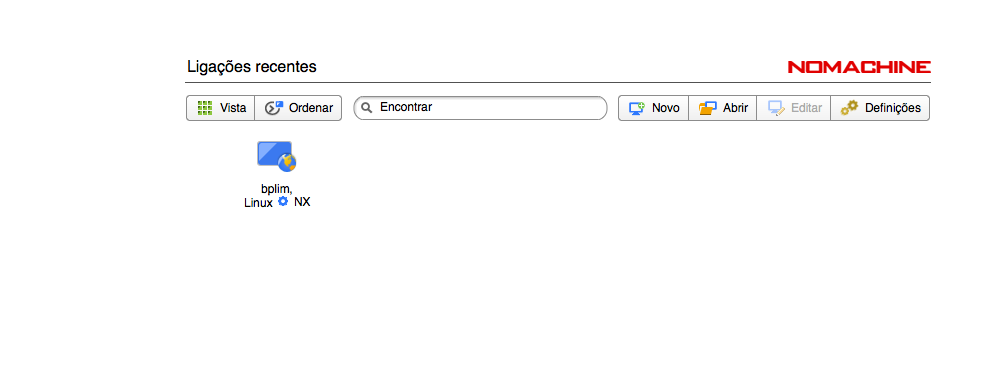
\includegraphics[width=4.72441in,height=1.72233in]{./media/image1.png}

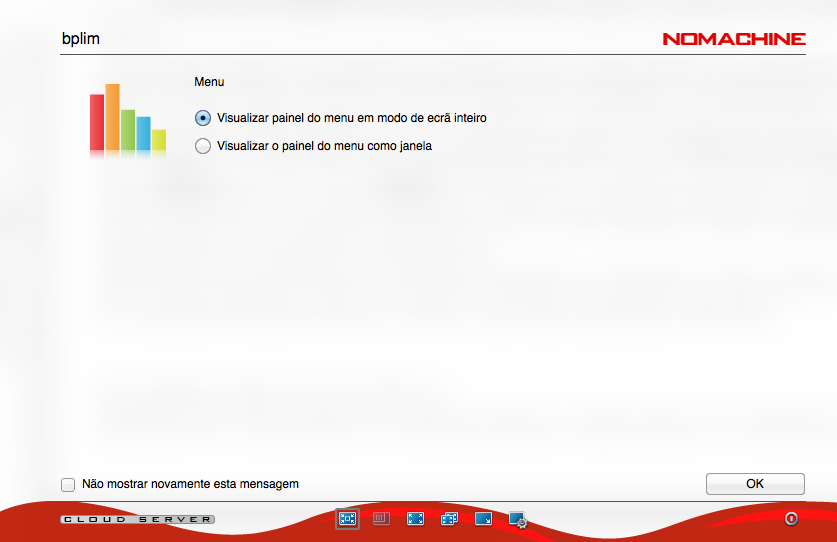
\includegraphics[width=4.72441in,height=3.05928in]{./media/image2.png}

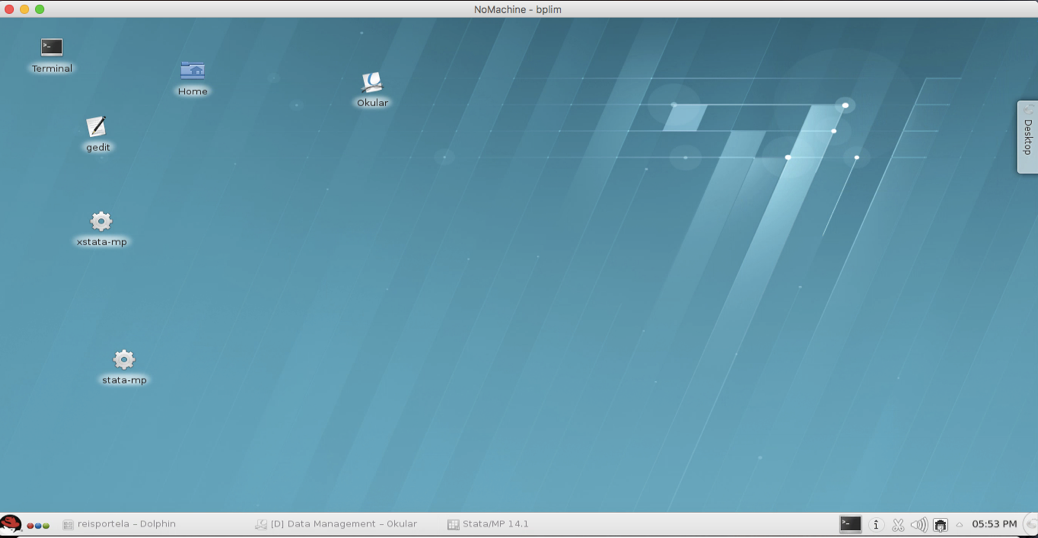
\includegraphics[width=4.72441in,height=2.44898in]{./media/image3.png}

\begin{enumerate}
\def\labelenumi{\arabic{enumi}.}
\setcounter{enumi}{3}
\tightlist
\item
  Select the ``\textbf{Kickoff Application Launcher}'' menu (in the lower left corner):
\end{enumerate}


\includegraphics[width=0.57067in,height=0.56371in]{./media/image4.png}

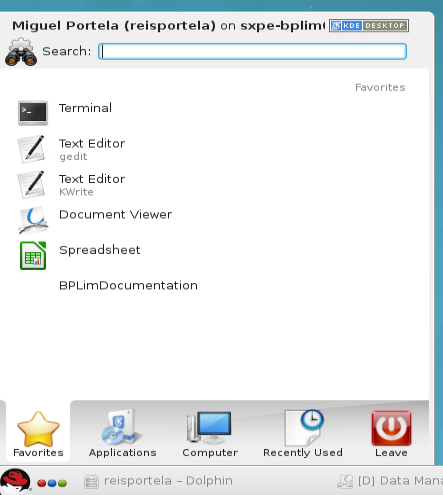
\includegraphics[width=2.3622in,height=2.63948in]{./media/image5.png}

\begin{enumerate}
\def\labelenumi{\arabic{enumi}.}
\setcounter{enumi}{4}
\tightlist
\item
  Then you should:
\end{enumerate}

\begin{itemize}
\tightlist
\item
  Click on the ``\textbf{Applications}'' button
\item
  Select \textbf{``BPLIM''} and click on your project (i.e., ``pxxx\_name''). At this stage, you should see a graphical environment (`Dolphin' application\footnote{For more information, see the manual on the Annual Data of Central Balance Sheet Database.}) like this:
\end{itemize}

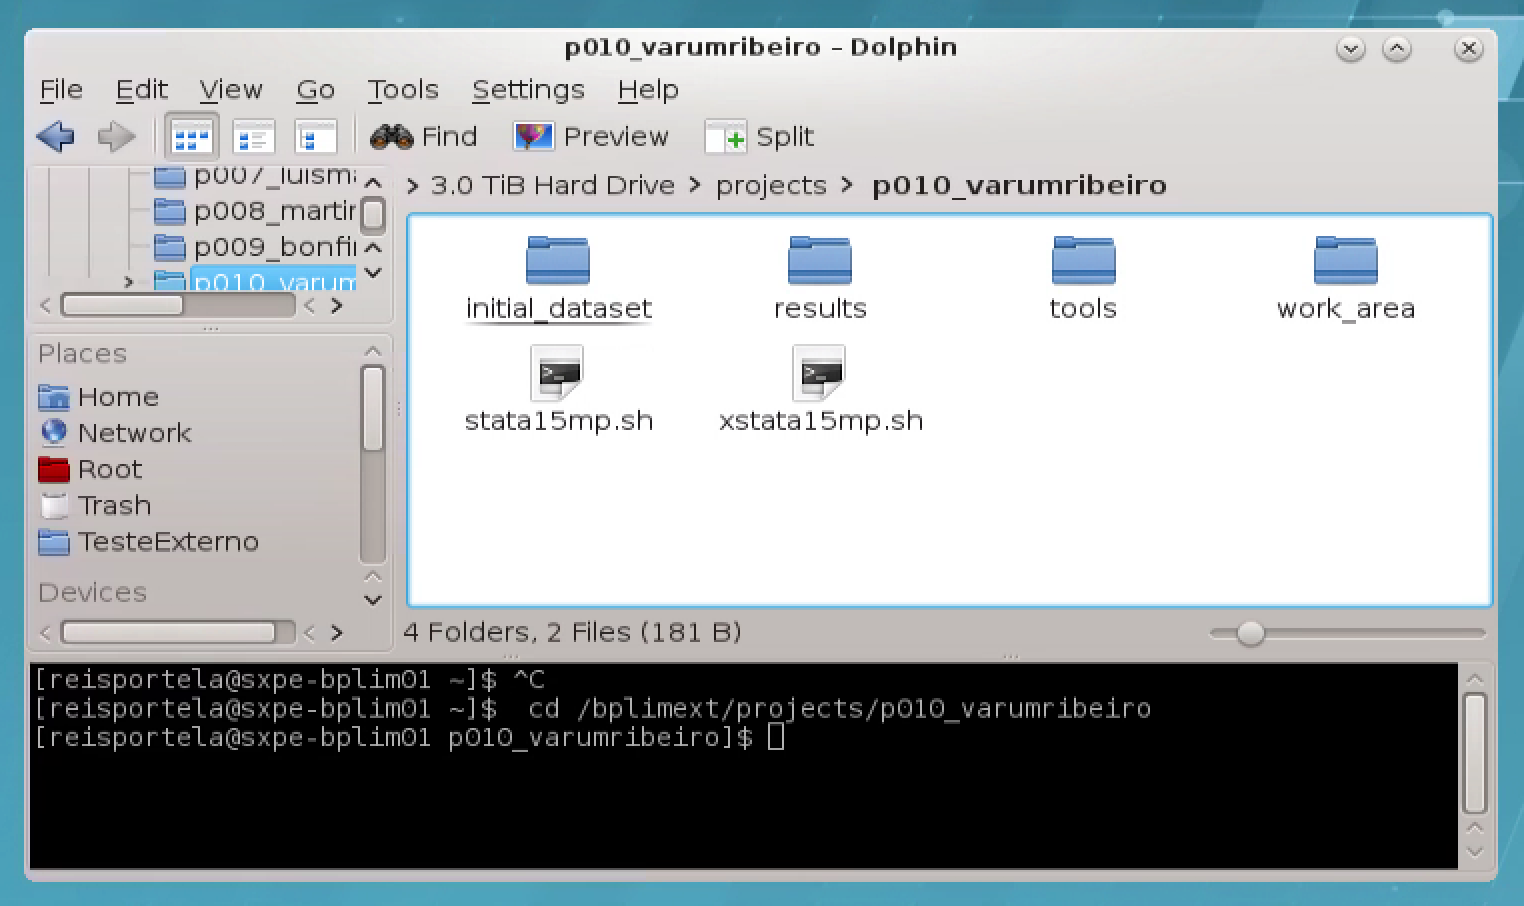
\includegraphics[width=4.72441in,height=2.80866in]{./media/image6.png}

You can see the prompt command line together with `Dolphin' using the
keyboard shortcut `F4'.

The directories that you have access to within the folder include:

\begin{longtable}[]{@{}ll@{}}
\toprule
\endhead
\begin{minipage}[t]{0.47\columnwidth}\raggedright
\textbf{initial\_dataset}\strut
\end{minipage} & \begin{minipage}[t]{0.47\columnwidth}\raggedright
Data sources provided by BPLIM.

\emph{You have
read-only access to this
directory.}\strut
\end{minipage}\tabularnewline
\begin{minipage}[t]{0.47\columnwidth}\raggedright
\textbf{results}\strut
\end{minipage} & \begin{minipage}[t]{0.47\columnwidth}\raggedright
Output files that
researchers wish to generate
and extract from the server.

\emph{You
have read-write access to this
directory.}\strut
\end{minipage}\tabularnewline
\begin{minipage}[t]{0.47\columnwidth}\raggedright
\textbf{tools}\strut
\end{minipage} & \begin{minipage}[t]{0.47\columnwidth}\raggedright
Specific analysis tools.

\emph{You have read-only access to
this directory.}\strut
\end{minipage}\tabularnewline
\begin{minipage}[t]{0.47\columnwidth}\raggedright
\textbf{work\_area}\strut
\end{minipage} & \begin{minipage}[t]{0.47\columnwidth}\raggedright
Temporary
work directory.

\emph{You have read-write
access to this directory.}\strut
\end{minipage}\tabularnewline
\bottomrule
\end{longtable}

\begin{itemize}
\item
  By default you also have two files (see image above): (1)
  stata15mp.sh; (2) xstata15mp.sh. Files with the
  "\textbf{{sh}}" extension allow you to send commands to
  your operating system or to enter your operating system for
  interactive use. The first one starts Stata version 15 in
  non-graphical mode, while the second launches Stata 15 in
  graphical mode. You can start both applications by typing in the
  Linux shell, for example, `xstata15mp.sh', or by double clicking
  the file name in `Dolphin'\footnote{To see the labels in English type the following command line in Stata: `label language en'.}
\item
  To reset and disconnect the remote desktop connection or session,
  you can simply log out your remote session, as shown on the
  screenshot below. After you log out, close the window.\footnote{A Micro-Entity is defined as a firm that falls below in at least two of the following criteria at the balance sheet date: i) total assets equal to 500.000 euros; ii) net turnover equal to 500.000 euros; or iii) average number of employees equal to 5. Small-sized Entities are firms satisfying at least two of the following conditions: i) total assets below 500.000 euros; ii) total gross sales and other income lower than 1.000.000 euros or; iii) average number of employees less than 20. For more details please check the manual on \href{../../CB/Jun2018/Pack_CB_Empresas_Jun18/manual_CB_Jun2018.html}{\emph{Central Balance Sheet Database - Annual Data}}.}
\end{itemize}

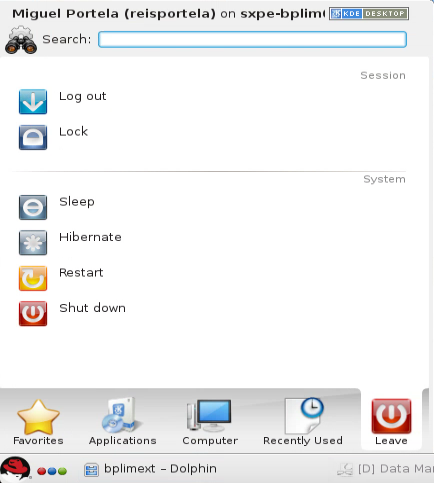
\includegraphics[width=3.14961in,height=3.50521in]{./media/image7.png}

Confirm before exiting by clicking on the \textbf{"Logout"} button to close the window\footnote{The relative changes are defined as the difference between the value of the variable observed in year t minus the value observed in the previous year. Relative changes are computed with respect to the average of year t and t-1 and are measured in percentage.}

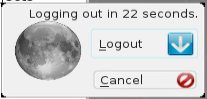
\includegraphics[width=1.14236in,height=0.52288in]{./media/image8.png}

\begin{itemize}
\tightlist
\item
  In case you do not logout, your session will be left open until your
  next login. You may use this facility to run your programs. However,
  one must be aware that this option uses resources from the server,
  so the efficient solution to run your programs ``over night'' is using
  the batch mode as described in Step 6 below. Furthermore, in case
  the server is rebooted during a maintenance procedure your session
  will be automatically close and unsaved documents will be lost. We
  recommend you save at regular intervals your statistical programs.
\end{itemize}

\hypertarget{using-the-shell-in-a-linux-operating-system}{%
\section{\texorpdfstring{{Using the `shell' in a Linux Operating System}}{Using the `shell' in a Linux Operating System}}\label{using-the-shell-in-a-linux-operating-system}}

If you wish to run your
programs in \textbf{\emph{{batch}}} mode, then you must use the
\emph{`\textbf{shell}'} of Linux. You can also use the `shell' to organize the
files in your working space.

\begin{enumerate}
\def\labelenumi{\arabic{enumi}.}
\tightlist
\item
  The \emph{`\textbf{shell}'}\footnote{In 2010 some declarations were reported according to \emph{Plano Oficial de Contas}. This situation occurs mostly for declarations sent in the cessation period and before or after the firms adopts a special fiscal period - a fiscal period different from calendar year.}
  {[}\^{}{[}5{]}\{.underline\}\^{}{]}(\url{https://translate.googleusercontent.com/\#footnote5})
  do Linux pode ser aberta a partir d e in Linux can be accessed from
\end{enumerate}

RedHat \textgreater{} ApplicationsApplications \textgreater{}\textgreater{} SystemSystem\textgreater{} \textgreater{}Terminal
Terminal

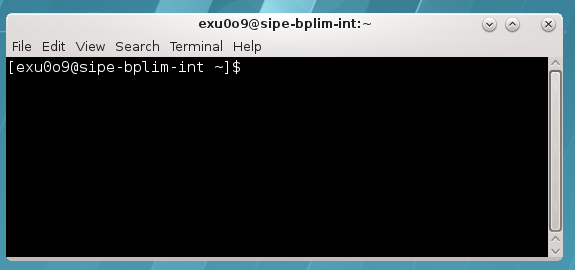
\includegraphics[width=3.93701in,height=1.84868in]{./media/image9.png}

\begin{enumerate}
\def\labelenumi{\arabic{enumi}.}
\setcounter{enumi}{1}
\item
  See the Appendix for a list of some of the most used commands.
\item
  In case you are using a non-English keyboard, the `true' keyboard
  might be different from the one you see. The changes apply mostly
  to the symbols, not letters or numbers. For example, in case you
  have a Portuguese keyboard on your computer the `+' is now in key
  `?', or the `*' is in SHIFT + ?. This issue is specific to the
  Operating System of your computer
\item
  Remember that Linux is case-sensitive: e.g., ``LS'' and ``ls'' are
  treated as different commands.
\item
  You can use the arrow keys to scroll up and down through the
  commands you've entered.
\item
  You can use the ``Tab'' key to complete the command line
  automatically.
\item
  E.g., type the following line to list elements within a folder in a
  `human readable' format, h, long list format, l, in reverse order,
  r, sort by modification time, t, and almost all files, A,

  ls -lArth
\end{enumerate}

\hypertarget{using-stata}{%
\section{\texorpdfstring{{Using Stata}}{Using Stata}}\label{using-stata}}

\begin{enumerate}
\def\labelenumi{\arabic{enumi}.}
\tightlist
\item
  Stata can be accessed in interactive graphical or non-graphical
  modes.\footnote{With the introduction of SNC some components that were previously classified as fixed tangible assets were reallocated to intangible assets to accommodate international standards. An example is highway concessions which were considered as tangible assets in POC and were reclassified as intangible assets in SNC.}
\end{enumerate}

\begin{itemize}
\item
  Interactive non-graphical mode

  Move to the desired folder, e.g.,

  cd /bplimext/projects/I001\_jdoe/

  and type

  /opt/bplimext/stata15/stata-mp
\end{itemize}

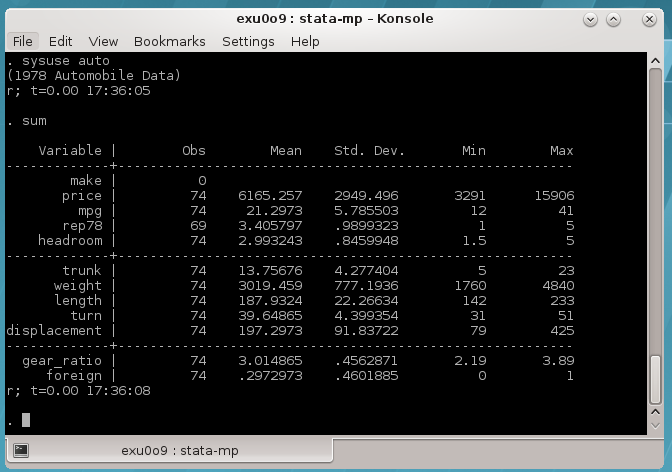
\includegraphics[width=3.54331in,height=2.4886in]{./media/image10.png}

\begin{itemize}
\item
  You may add a `path' to your system folder by typing, for the
  example on Stata 15, the following command in the shell

  PATH = \$PATH:/opt/bplimext/stata15
\item
  For the interactive graphical mode click on the icons
  ``\textbf{{xstata14mp.sh}}'' (Stata 14) or
  ``\textbf{{xstata15mp.sh}}'' (Stata 15) located in the
  `desktop', depending on the desired Stata version,
\end{itemize}

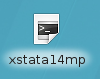
\includegraphics[width=0.59055in,height=0.46654in]{./media/image11.png}

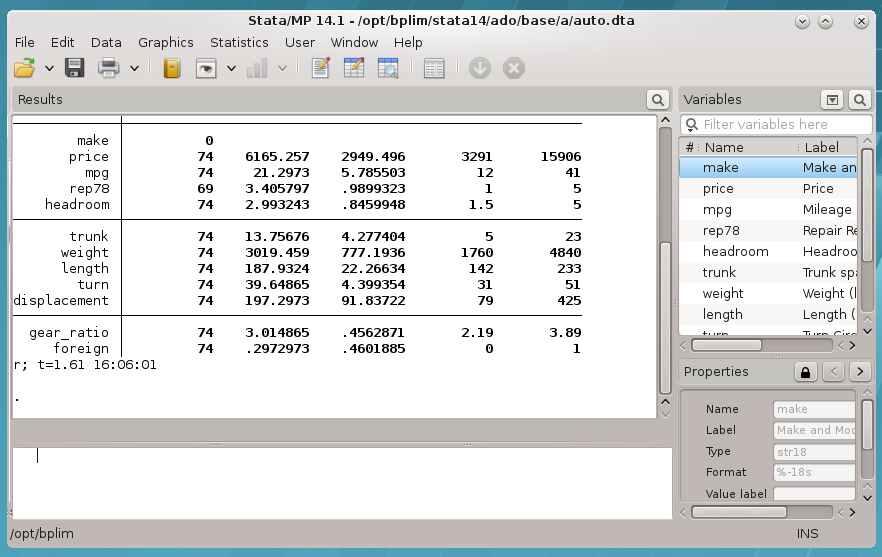
\includegraphics[width=3.93701in,height=2.48638in]{./media/image12.png}

\begin{verbatim}
- You can use the 'Do-file Editor' in Stata to create your own
  "do-files" and "ado-files", or alternatively you can use
  **KWrite** editor (or 'gedit'). Poder á abri-lo a partir de
  **[RedHat]{.underline}** \>

- You can open it from **RedHat** \> **Applications**
  **Applications** \>\> **Utilities** **Utilities** \> \> **KWrite**
  . **KWrite**. You can also launch 'KWrite' from the 'shell' by
  typing 'kwrite'
\end{verbatim}

\begin{itemize}
\tightlist
\item
  In case the icon is not in your desktop, use Dolphin, move to folder
  `/opt/bplimext/stata15', and drag and drop the file `xstata-mp' into
  the desktop
\end{itemize}

\begin{enumerate}
\def\labelenumi{\arabic{enumi}.}
\setcounter{enumi}{1}
\tightlist
\item
  To look for \textbf{``ado-files''}:
\end{enumerate}

``Ado-files'' are text files containing the Stata program. It is
advisable that one create and save his/her ``ado-files'' so the results
can be replicated later by running the saved ``ado-files'' on the
BPLIM's datasets.

Stata looks for ``ado-files'' in several places. When it comes to
personal ado-directories, they can be categorized in four ways:

\begin{itemize}
\item
  (SITE), the directory for ``ado-files'' your site might have
  installed;
\item
  (PLUS), the directory for ``ado-files'' you personally might have
  installed;
\item
  (PERSONAL), the directory for ``ado-files'' you might have written;
\item
  (OLDPLACE), the directory where Stata users used to save their
  personally written ado-files.
\end{itemize}

The ado-files you have just written or those created for this project
can be found in the current directory (.).

Specific `ado-files' you may ask to be made available in the server
will be placed in your folder
`/bplimext/projects/YOURPROJECTID/tools'. You should add this folder
to your Stata `ado-files' folder by executing the following command
within Stata,

sysdir set PERSONAL ``/bplimext/projects/YOURPROJECTID/tools''

You may also edit your `profile.do' file, located in your root folder,
``/home/YOURPROJECTID/'', and add key instructions you may want to be
executed every time you start Stata. The above instruction is one of
such cases. You can create, or edit, the file `profile.do' using
`Do-file Editor' within Stata (`vi profile.do' or KWrite are also a
possibility).

The \textbf{\emph{sysdir}} command within Stata will tell you where they are on
your computer:

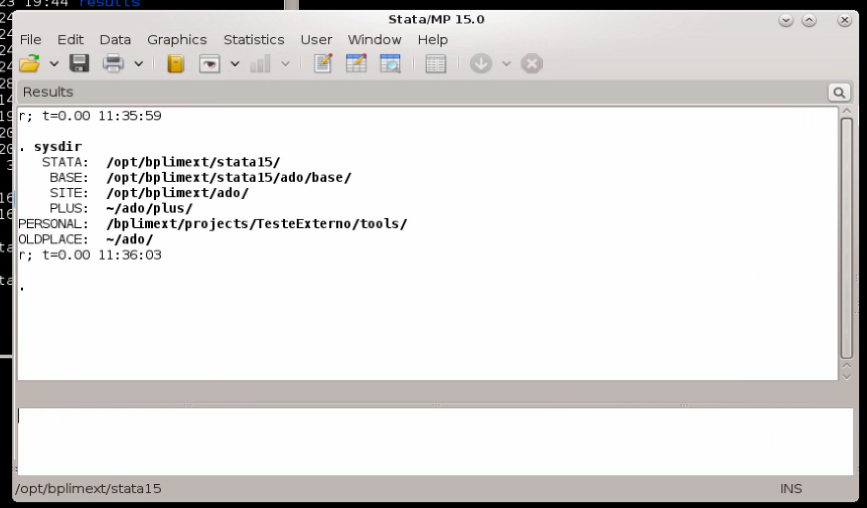
\includegraphics[width=3.93681in,height=2.27514in]{./media/image13.png}

\hypertarget{stata-in-batch-mode}{%
\section{\texorpdfstring{{Stata in `batch' mode}}{Stata in `batch' mode}}\label{stata-in-batch-mode}}

\begin{enumerate}
\def\labelenumi{\arabic{enumi}.}
\tightlist
\item
  Start a \emph{'\textbf{shell}'} in Linux and navigate to the directory
  of the ``do-file'' file that you want to run (ex: prog1.do)
\end{enumerate}

\textbf{cd /bplim/projects/I001\_jdoe/work\_area/} cd
/bplimext/projects/I001\_jdoe/work\_area/

\begin{enumerate}
\def\labelenumi{\arabic{enumi}.}
\setcounter{enumi}{1}
\tightlist
\item
  You might find it easier to use `Dolphin' (= File Manager) to move
  over your folder structure. In this case, we recommend activating
  the `shell' (= `Terminal') associated with `Dolphin'
\end{enumerate}

\begin{itemize}
\item
  use Dolphin/File Manager
\item
  click `F4' to activate the shell with Dolphin. Benefit: fast
  transition within folders and, at the same time, the ability
  to run shell commands
\end{itemize}

\begin{enumerate}
\def\labelenumi{\arabic{enumi}.}
\setcounter{enumi}{2}
\item
  Create an ASCII file named, e.g., `batch\_prog1'
\item
  Inside the file write just a line with the execution command you
  would type in the `shell'; e.g.,

  /opt/bplimext/stata15/stata-mp do
  /bplimext/projects/BPlim\_inicial/work\_area/prog1.do
\item
  You can use, for example, the command line app `vi' to create the batch file
\end{enumerate}

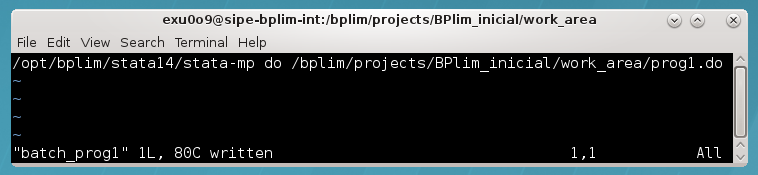
\includegraphics[width=3.54331in,height=0.81802in]{./media/image14.png}

\begin{enumerate}
\def\labelenumi{\arabic{enumi}.}
\setcounter{enumi}{5}
\tightlist
\item
  The batch file can also be created using apps like `kwrite' or Stata
  `do file editor'
\end{enumerate}

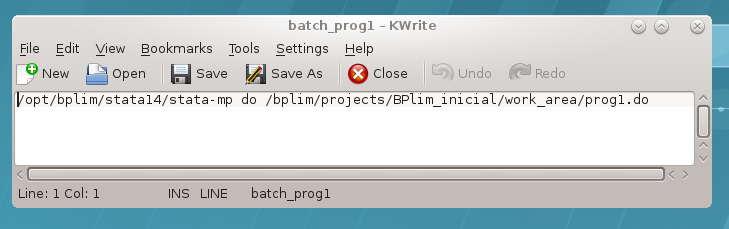
\includegraphics[width=3.54331in,height=1.11324in]{./media/image15.png}

or

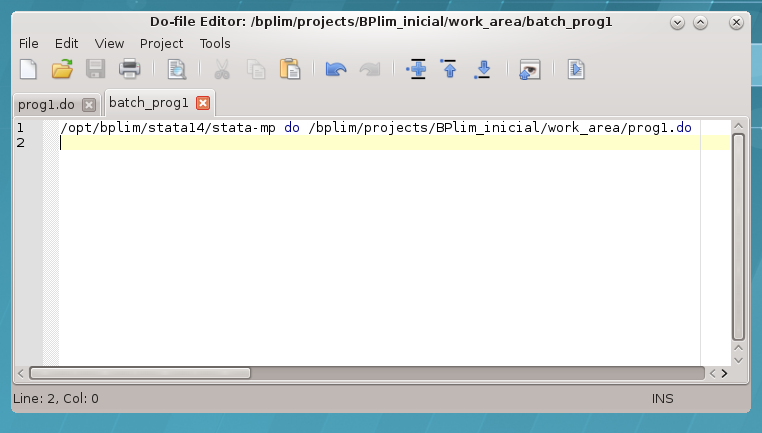
\includegraphics[width=3.54331in,height=2.01342in]{./media/image16.png}

\begin{enumerate}
\def\labelenumi{\arabic{enumi}.}
\setcounter{enumi}{6}
\item
  You may add the extension `.txt' to the name of the batch file, as
  sometimes Stata \emph{doeditor} does not `see' the file `batch', while
  it `sees' `batch.txt'
\item
  Once the batch file is created one runs the .do file in batch mode
  by typing in the `Terminal':

  at now --f batch.txt
\item
  Type `man at' to see further option of the command `at'; e.g., one
  could type

  at now + 5 hours --f batch.txt
\end{enumerate}

or

\begin{verbatim}
at now + 4 minutes --f batch\_prog1
\end{verbatim}

to run the Stata program within 5 hours or 4 minutes from now,
respectively. `man' is the help function in Linux

\begin{enumerate}
\def\labelenumi{\arabic{enumi}.}
\setcounter{enumi}{9}
\item
  Type `top' in the shell/Terminal to confirm the program is running
\item
  Under `top' type `i' to hide irrelevant processes (show less output)
\item
  To kill a running process with `top' press `k', for `kill', write
  \textgreater{} the process number and then type `9'. The process number is
  \textgreater{} identified in the first column as PID
\item
  To get out of the top, type `q'
\item
  Useful features of the command `at':
\end{enumerate}

\begin{itemize}
\item
  `atq': use it to see programs in the batch queue (an `=' sign
  indicates the program is running; an `a' indicates it is in
  the queue and we see the time when it will be executed)
\item
  `atrm \#': remove a batch from the batch queue
\item
  one can see how the batch is running by typing

  `tail --f logcrc\_may21.log'
\end{itemize}

It allows you to see an updated version of the last lines of the log;
\emph{i.e.}, it updates each time the log is changed by Stata. A key
advantage of tail is that it does not interfere with the log file,
namely it does not write over it.

\begin{enumerate}
\def\labelenumi{\arabic{enumi}.}
\setcounter{enumi}{14}
\tightlist
\item
  Another way to run a program in the background is by using the
  command `screen'
\end{enumerate}

\begin{itemize}
\item
  `screen' is useful when one wants to run Stata in interactive
  mode and still guarantee that if the network connection goes
  down one does not lose the session. We can simply kill the
  `NoMachine' session and recover it later by typing `screen
  --r'
\item
  We can run several instances of screen. If this is the case,
  after opening a new NoMachine session we need to type in the
  Terminal shell `screen --d' to identify the running background
  sessions. We can retrieve a particular session by knowing the
  `pid' number and typing `screen --r 34176'
\end{itemize}

\hypertarget{additional-statistical-software}{%
\section{\texorpdfstring{{Additional Statistical Software}}{Additional Statistical Software}}\label{additional-statistical-software}}

You can also use `R' and `python' by issuing in the shell the
respective designation. Both applications can only be used in the
`shell'. You can check the packages available in R by tipping
`installed.packages()'.

\hypertarget{allowed-outputs}{%
\section{\texorpdfstring{{Allowed outputs}}{Allowed outputs}}\label{allowed-outputs}}

Stata results can be exported to a file on disk using one of the following formats:

\begin{enumerate}
\def\labelenumi{\arabic{enumi}.}
\item
  ASCII files: e.g., log files
\item
  graphs: as .PNG (do not use the option save, or saving, within a
  graph command; instead, use the separate command line `graph export
  xyz.png')
\item
  csv: CSV (Comma Separated Value format), e.g., for use with MS Excel
\item
  rtf: Rich Text Format for use with word processors
\item
  xls or xlsx: Excel files with output tables
\item
  tex: Latex format
\end{enumerate}

\hypertarget{remove-outputs}{%
\section{\texorpdfstring{{Remove outputs}}{Remove outputs}}\label{remove-outputs}}

Place in the ``{results}'' folder all the outputs you want
to remove from the server.\footnote{This variable has no match in \emph{Plano Oficial de Contas}.}

\begin{enumerate}
\def\labelenumi{\arabic{enumi}.}
\item
  Send an email with the title
  ``\textbf{project I001\_jdoe}: request for result extraction'' to
  ``\textbf{{bplim@bportugal.pt}}''.
\item
  Upon validation, the results will be sent to you via email.
\end{enumerate}

\hypertarget{scientific-support}{%
\section{\texorpdfstring{{Scientific Support}}{Scientific Support}}\label{scientific-support}}

Researchers will be provided with the necessary scientific and
computational support (\emph{i.e.}, advises on programming, computational
resources, micro econometrics, and econometrics of panel data for
research undertaken with the selected Microdata).

\hypertarget{appendix-1-basic-shell-commands-on-linux}{%
\section{\texorpdfstring{{Appendix 1 -- Basic `shell' Commands on Linux}}{Appendix 1 -- Basic `shell' Commands on Linux}}\label{appendix-1-basic-shell-commands-on-linux}}

\begin{itemize}
\item
  \textbf{top} List the procedures that are being executed on the
  server

  \begin{itemize}
  \item
    clicar em ' i ' para omitir processos adormecidos; press 'i'
    \textgreater{} option to omit background processes;
  \item
    clicar press ' h ' para \textbf{\emph{help on top options}} ; 'h'
    \textgreater{} option to obtain the \textbf{top command help}.
  \end{itemize}
\item
  \textbf{pwd} Show current working
  directory
\item
  \textbf{cd} Change directory

  cd /bplimext/projects/I001\_jdoe/work\_area/

  `cd \textasciitilde{}' moves to your home folder
\end{itemize}

\begin{itemize}
\item
  \textbf{cp}cp Copy file(s) to a given path

  cp prog1.do /bplimext/projects/I001\_jdoe/results
\end{itemize}

\begin{itemize}
\item
  \textbf{mv}mv Move file(s) or rename a file from a given path

  mv prog1.do /bplimext/projects/I001\_jdoe/results
\end{itemize}

\begin{itemize}
\item
  \textbf{rm}rm Delete a file

  rm /bplimext/projects/I001\_jdoe/results/prog1.do
\end{itemize}

\begin{itemize}
\item
  \textbf{mkdir}mkdir Creates a directory

  mkdir programas
\end{itemize}

\begin{itemize}
\item
  \textbf{rmdir}rmdir Deletes a directory

  rmdir programas
\end{itemize}

\begin{itemize}
\item
  \textbf{screen}screen Switch between screen

  screen top
\end{itemize}

\begin{itemize}
\item
  \textbf{stata} -- \textbf{mpman}man Show the manual page for the given command

  man ls
\end{itemize}

\begin{itemize}
\tightlist
\item
  \textbf{du}du -h Check the information of disk usage of files and
  directories.
\end{itemize}

\begin{quote}
The ``\textbf{-h}'' option with ``\textbf{du}'' command provides results in ``Human
Readable Format''.
\end{quote}

Ex: du /bplimext/projects/I001\_jdoe/work\_area/

\begin{itemize}
\item
  \textbf{df}df -h Check disk space utilization and show the disk space
  \textgreater{} statistics in ``human readable'' format.
\item
  vi View `ASCII' files; e.g., log files
\item
  \textbf{ghostscript} Preview files with the extensions of \textbf{.eps} and
  \textbf{.pdf}
\end{itemize}

\begin{quote}
ghostscript /bplimext/projects/I001\_jdoe/results/`file\_name.pdf'
\end{quote}

\begin{itemize}
\item
  okular View `PDF'
\item
  find Find files
\end{itemize}

\begin{quote}
Structure: find /path option filename

find . --name ``*.do''

Send the `find' output to a file:

find . --name ``*.do'' \textgreater{} find\_results.txt

Look for a particular string within the `find' output:

find . --name ``*.do'' \textbar{} grep ``analise''

Identify files with extension `.do' that \textbf{contain} the word `graph':

find . --name ``*.do'' -exec grep ``graph export'' `\{\}' \textbackslash{}; -print
\end{quote}

\begin{itemize}
\item
  passwd Change your password
\item
  \textbf{To exit} a program, type \textbf{CTRL + C} (`CTRL + C' kills a particular
  execution in the shell)
\end{itemize}

\hypertarget{appendix-2-using-the-vi-file-editor}{%
\section{\texorpdfstring{{Appendix 2 -- Using the `vi' file editor}}{Appendix 2 -- Using the `vi' file editor}}\label{appendix-2-using-the-vi-file-editor}}

\begin{enumerate}
\def\labelenumi{\arabic{enumi}.}
\item
  In the shell type `vi batch1.txt'
\item
  This are the main shortcut keys

  \begin{enumerate}
  \def\labelenumii{\alph{enumii}.}
  \item
    `i' insert text
  \item
    `ESC' key get out of the `insert' mode
  \item
    `x' delete specific characters
  \item
    `dd' delete a full line
  \item
    `10 dd' delete 10 lines
  \item
    `yy' copy lines
  \item
    `p' paste lines
  \item
    `SHIFT + G' go to the last line
  \item
    `gg' goes to the first line
  \item
    `ESC + q!' exit `vi' without writing
  \item
    `w!' write and replace the file
  \item
    `ESC + q' exit the `vi' session
  \item
    Check, for example,
    \url{https://www.cs.colostate.edu/helpdocs/vi.html}
  \end{enumerate}
\item
  Much easier solution: call `gedit' file editor
\item
  Linux commands I have to add to the manual
\item
  `CTRL + R': allows me to recover a previous command
\item
  vi .bash\_history
\end{enumerate}

\hypertarget{appendix-3-external-servers-password-requirements}{%
\section{\texorpdfstring{{Appendix 3 -- External server's password requirements}}{Appendix 3 -- External server's password requirements}}\label{appendix-3-external-servers-password-requirements}}

\begin{longtable}[]{@{}lll@{}}
\toprule
\endhead
\begin{minipage}[t]{0.30\columnwidth}\raggedright
\textbf{Rule}\strut
\end{minipage} & \begin{minipage}[t]{0.30\columnwidth}\raggedright
\textbf{Value}\strut
\end{minipage} & \begin{minipage}[t]{0.30\columnwidth}\raggedright
\textbf{Notes }\strut
\end{minipage}\tabularnewline
\begin{minipage}[t]{0.30\columnwidth}\raggedright
Maximum Password
Lifetime\strut
\end{minipage} & \begin{minipage}[t]{0.30\columnwidth}\raggedright
\textbf{{60
days}}\strut
\end{minipage} & \begin{minipage}[t]{0.30\columnwidth}\raggedright
\textbf{{After 60 days the
password will
expire}}
and has to be changed
in the next login.
The password can be
changed at any moment
using: \textbf{(1)}, ``All
Applications \textbar{}
Settings \textbar{} System
Settings -- Account
Details'', click
``Change Password'';
or, \textbf{(2)}, in the
`Shell' type `passwd'\strut
\end{minipage}\tabularnewline
\begin{minipage}[t]{0.30\columnwidth}\raggedright
Minimum Number of
Character Classes\strut
\end{minipage} & \begin{minipage}[t]{0.30\columnwidth}\raggedright
4\strut
\end{minipage} & \begin{minipage}[t]{0.30\columnwidth}\raggedright
You should include at
least 4 classes of
characters in the
password. For
example, small
letters, capital
letters, numbers and
punctuation marks.

There are a total of
five classes:

\begin{quote}
1. Capital letters
:
A-Z

2. Small letters:
a-z

3. Numbers: 1-9

4. Punctuation
marks: \textless{}space\textgreater{} !
\% \& ( ) * + . , \{
\} \[ \] \textasciitilde{} " \# \$
' - / \textbackslash{} \^{} \_ `
\textbar{}

5. Characters abov
e
127 (0x7F): marked
characters (ã, á,
ä, à, etc.);
symbols (@, £, §,
º, ª, «, », etc.)
\end{quote}

Number of characters:
by using the same
character 3 or more
times may imply the
use of an additional
class (it is highly
recommended that you
do not use
consecutively the
same character more
than 2 times)\strut
\end{minipage}\tabularnewline
\begin{minipage}[t]{0.30\columnwidth}\raggedright
Minimum Length of
Password\strut
\end{minipage} & \begin{minipage}[t]{0.30\columnwidth}\raggedright
8\strut
\end{minipage} & \begin{minipage}[t]{0.30\columnwidth}\raggedright
The minimum size of
the password is 8
characters (it may be
higher in case you
repeat characters)\strut
\end{minipage}\tabularnewline
\begin{minipage}[t]{0.30\columnwidth}\raggedright
Password History\strut
\end{minipage} & \begin{minipage}[t]{0.30\columnwidth}\raggedright
7\strut
\end{minipage} & \begin{minipage}[t]{0.30\columnwidth}\raggedright
One cannot use a
password defined in
the previous set of 7
passwords\strut
\end{minipage}\tabularnewline
\begin{minipage}[t]{0.30\columnwidth}\raggedright
Maximum Consecutive
Failures\strut
\end{minipage} & \begin{minipage}[t]{0.30\columnwidth}\raggedright
6\strut
\end{minipage} & \begin{minipage}[t]{0.30\columnwidth}\raggedright
If the user fails 6
consecutive times the
password the account
will be locked for
the time defined in
``Lockout Time''\strut
\end{minipage}\tabularnewline
\begin{minipage}[t]{0.30\columnwidth}\raggedright
Fail Interval\strut
\end{minipage} & \begin{minipage}[t]{0.30\columnwidth}\raggedright
60 sec.\strut
\end{minipage} & \begin{minipage}[t]{0.30\columnwidth}\raggedright
Time interval for
attempts to enter a
password to be
considered
consecutive. If more
than 60 seconds have
elapsed since the
last attempt,
consecutive attempts
are no longer
considered, ie the
number of failures,
according to the
requirement "Maximum
Consecutive
Failures" becomes
one.\strut
\end{minipage}\tabularnewline
\begin{minipage}[t]{0.30\columnwidth}\raggedright
Lockout Time\strut
\end{minipage} & \begin{minipage}[t]{0.30\columnwidth}\raggedright
600 sec.\strut
\end{minipage} & \begin{minipage}[t]{0.30\columnwidth}\raggedright
Time (10 minutes)
during which the
account will be
locked if the maximum
number of failed
attempts is reached.\strut
\end{minipage}\tabularnewline
\bottomrule
\end{longtable}

\hypertarget{appendix-4-download-install-and-configure-nomachine-client}{%
\section{\texorpdfstring{{Appendix 4 -- Download, install and configure NoMachine client}}{Appendix 4 -- Download, install and configure NoMachine client}}\label{appendix-4-download-install-and-configure-nomachine-client}}

\textbf{Step 1}: go to the link below and use the credentials provided by
BPLIM to access the site. \textbf{Note}: sometimes the internet provider,
\emph{e.g.}, an University, may block the access to this particular web site.
Please check with your provider in case you get an error while trying to
use the link.

\url{https://www.bportugal.pt/webdrive/index.php/s/irAzxZmir8KHyzD/authenticate}

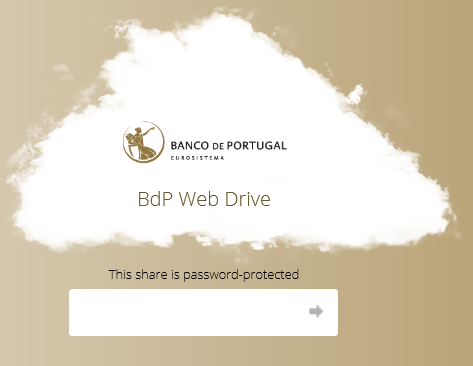
\includegraphics[width=3.0528in,height=2.3622in]{./media/image17.png}

\textbf{Step 2}: download the file with an extension compatible with your OS
(Operation System)

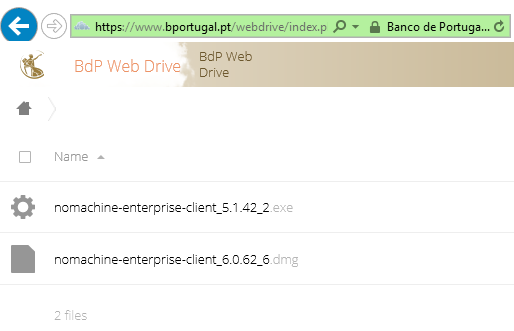
\includegraphics[width=3.6682in,height=2.3622in]{./media/image18.png}

\textbf{Step 3}: install `NoMachine'

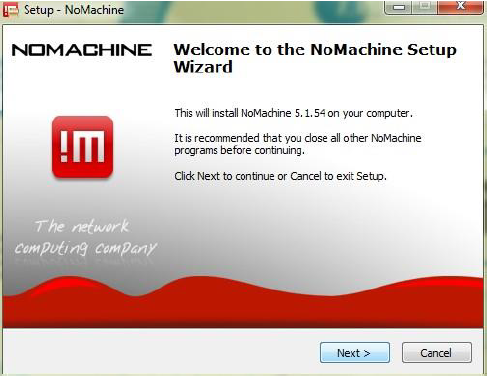
\includegraphics[width=4.07941in,height=3.14961in]{./media/image19.png}

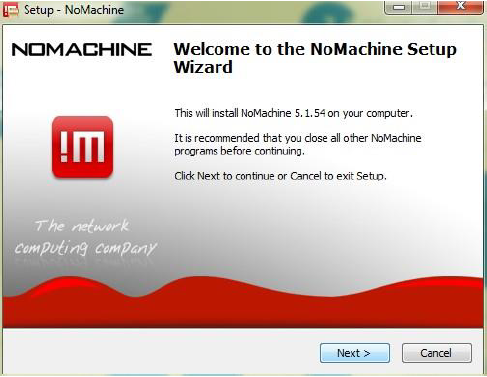
\includegraphics[width=4.06859in,height=3.14961in]{./media/image20.png}

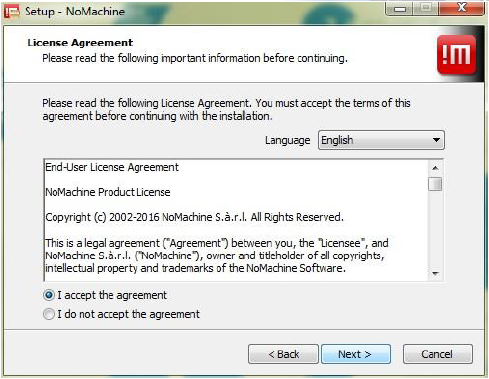
\includegraphics[width=4.06374in,height=3.14961in]{./media/image21.png}

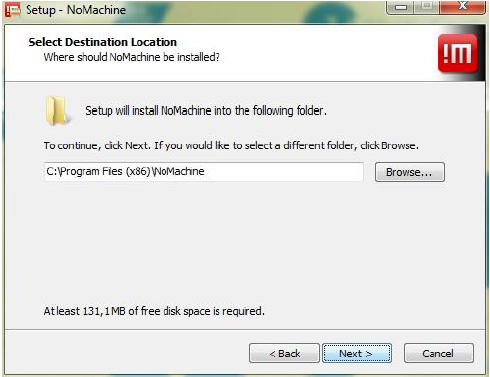
\includegraphics[width=4.09365in,height=3.14961in]{./media/image22.png}

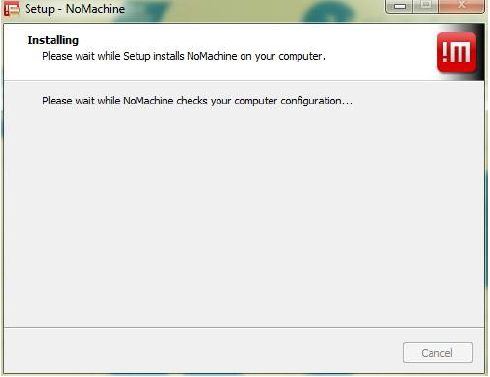
\includegraphics[width=4.09365in,height=3.14961in]{./media/image23.png}

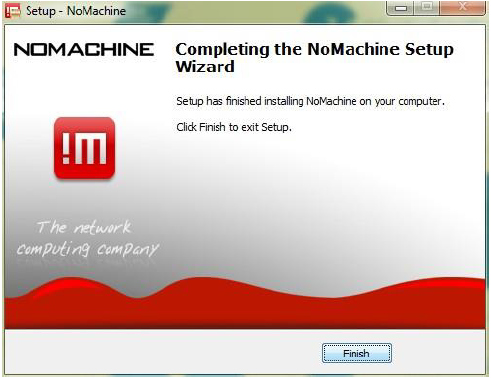
\includegraphics[width=4.09115in,height=3.14961in]{./media/image24.png}

\textbf{\\
}

\textbf{Step 4}: reboot your computer

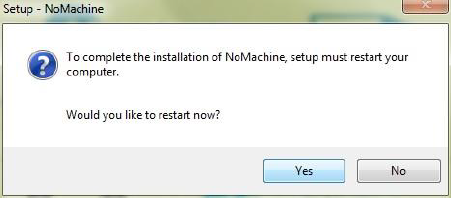
\includegraphics[width=2.75591in,height=1.21602in]{./media/image25.png}

\textbf{Step 5}: NoMachine client access configuration

\textbf{Step 5.1}: start `NoMachine' and create a new connection

\begin{quote}
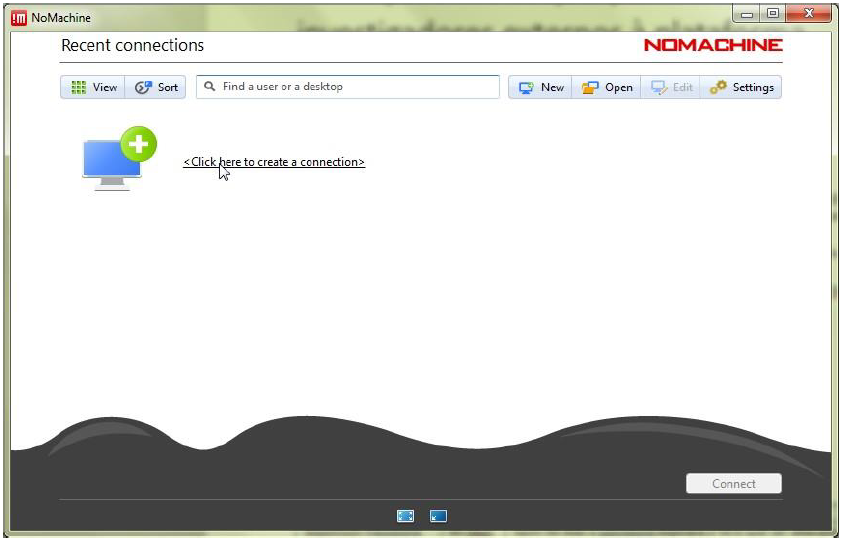
\includegraphics[width=4.72441in,height=3.02971in]{./media/image26.png}
\end{quote}

\textbf{Step 5.2}: Choose `NX protocol'

\begin{quote}
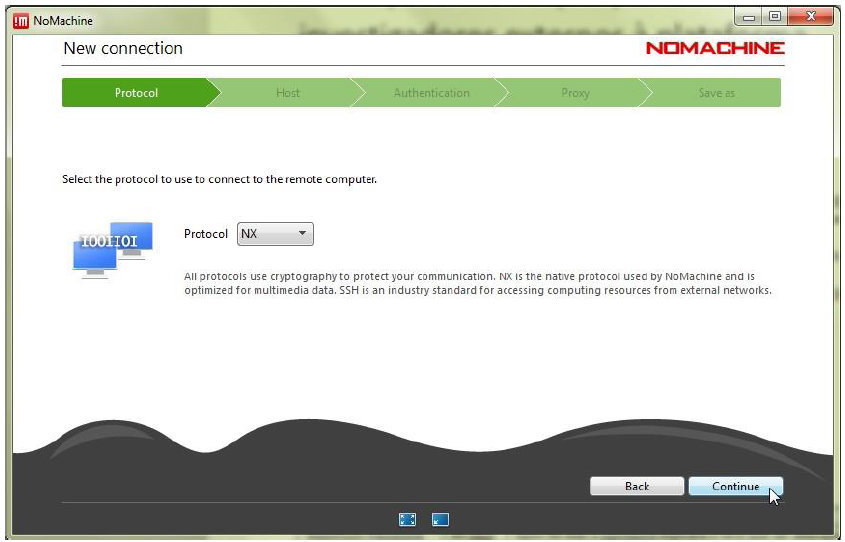
\includegraphics[width=4.72441in,height=3.0302in]{./media/image27.png}
\end{quote}

\textbf{Step 5.3}: Define the `Host' as bplim.bportugal.pt, `Port' 4000

\begin{quote}
Click `Use UDP communication for multimedia data'

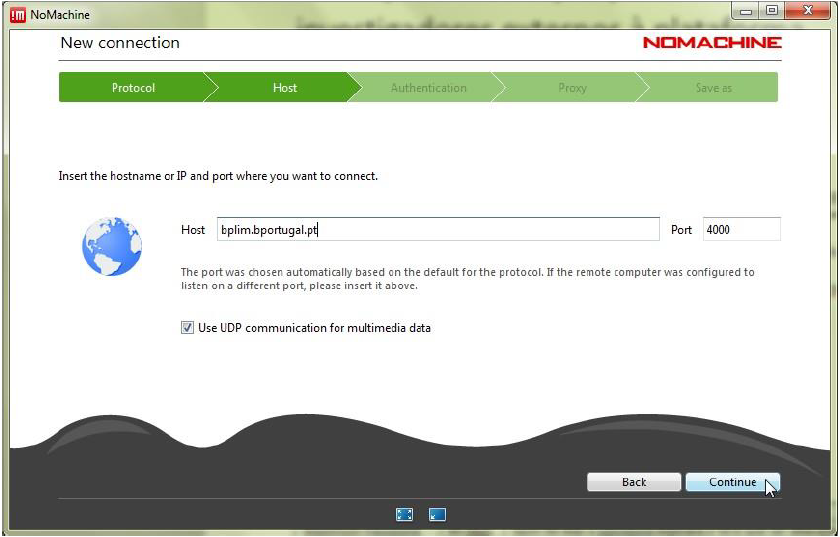
\includegraphics[width=4.72441in,height=3.02002in]{./media/image28.png}

\textbf{Step 5.4}: Use password authentication, with or without proxy,
depending on the instructions of the network administrator / user's
computer support, with the name ``BPLIM-LabInvestMicrodados Banco de
Portugal''.

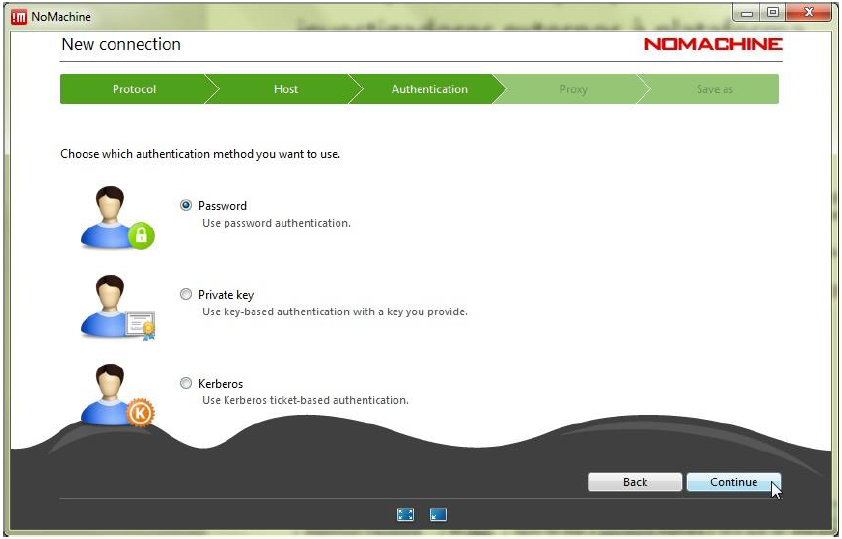
\includegraphics[width=4.72441in,height=3.02438in]{./media/image29.png}

\textbf{Step 5.5}: Do not use a `proxy'

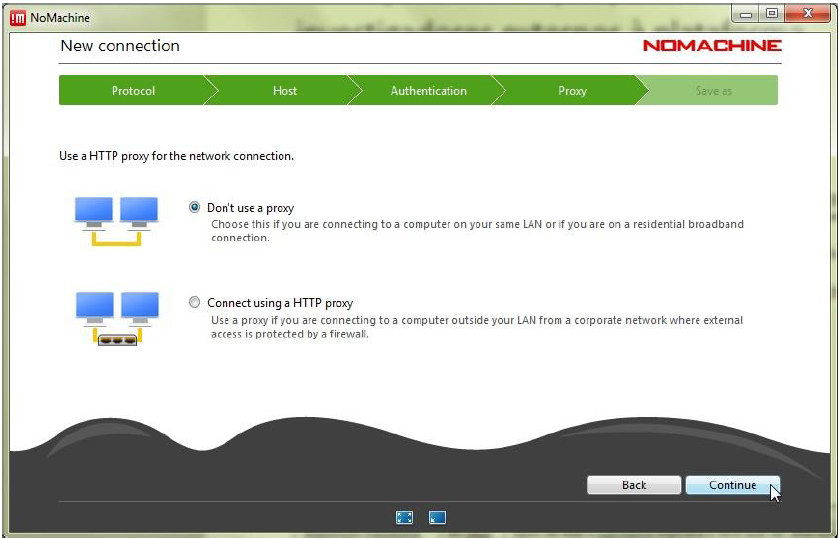
\includegraphics[width=4.72441in,height=3.03165in]{./media/image30.png}

\textbf{Step 5.6}: Define a name for the connection

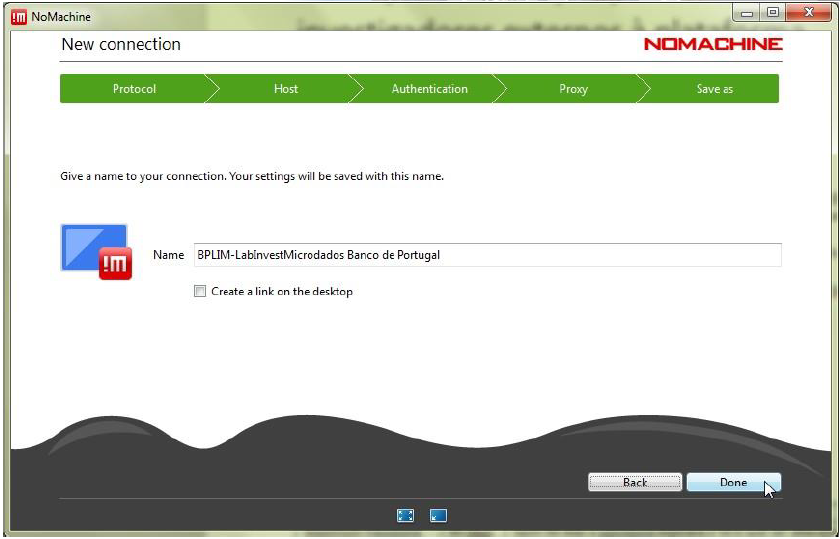
\includegraphics[width=4.72441in,height=3.03165in]{./media/image31.png}

\textbf{Step 5.7}: Once the entry for bplim.bportugal.pt has been created,
connect:

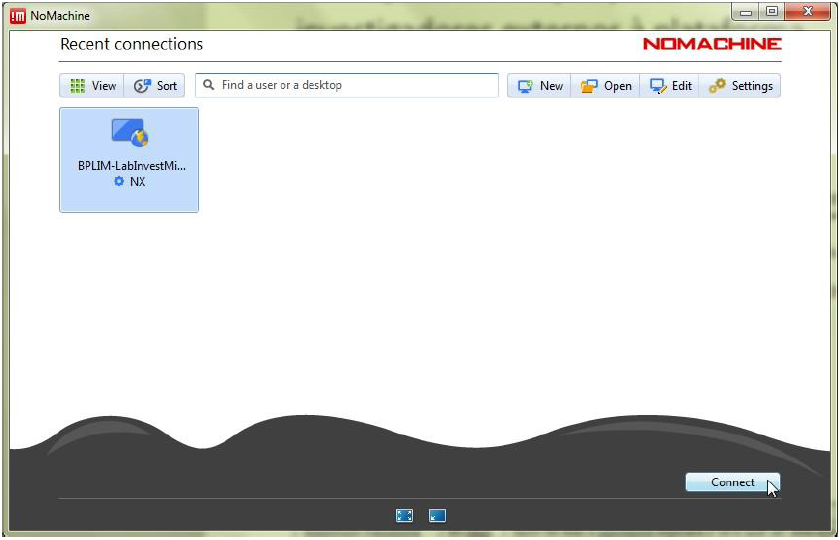
\includegraphics[width=4.72441in,height=3.03698in]{./media/image32.png}
\end{quote}

\textbf{\\
}

\begin{quote}
\textbf{Step 5.8}: Before the first effective connection it may be
necessary to accept the certificate from bplim.bportugal.pt

The Investigator should verify that the "fingerprint" (verification
code) is:

\textbf{29 DC CC 9E 8B 87 23 B1 76 28 8D 29 3F D0 E3 EB 4E 73 76 9D}

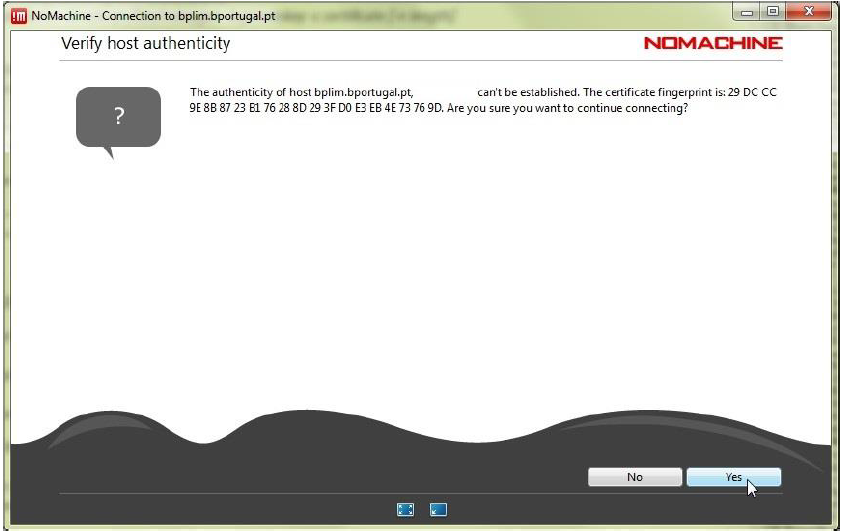
\includegraphics[width=4.72441in,height=2.98511in]{./media/image33.png}
\end{quote}

\textbf{\\
}

\begin{quote}
\textbf{Step 5.9}: Connect with the UserID (\textbf{case sensitive}) and
password provided by Banco de Portugal:

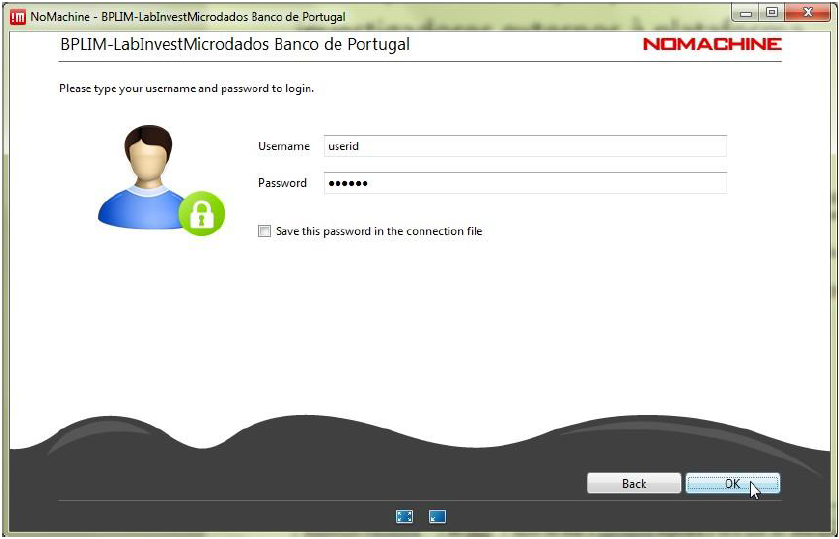
\includegraphics[width=4.72441in,height=3.03504in]{./media/image34.png}

\textbf{Step 5.10}: After the first successful login, it is necessary to
change the password, which must comply with the Password Policy
defined above.

If the new password does not comply with the Password Policy, the
original password provided by the Banco de Portugal will be
re-requested. See Appendix 3 for details.

The NoMachine client does not tell you why the new password was not
accepted -- it is the responsibility of the user to verify that the
new password is in compliance.

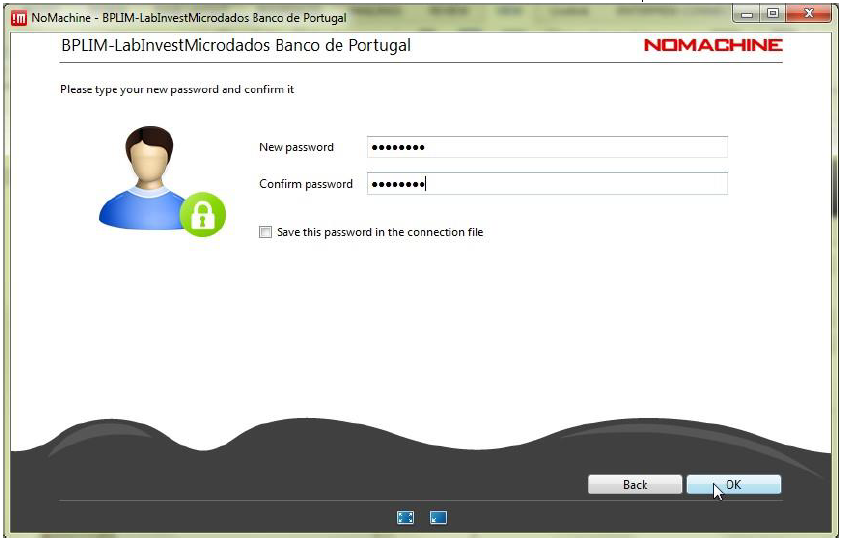
\includegraphics[width=4.72441in,height=3.02972in]{./media/image35.png}

\textbf{Step 5.11}: Upon login success the following screens should appear

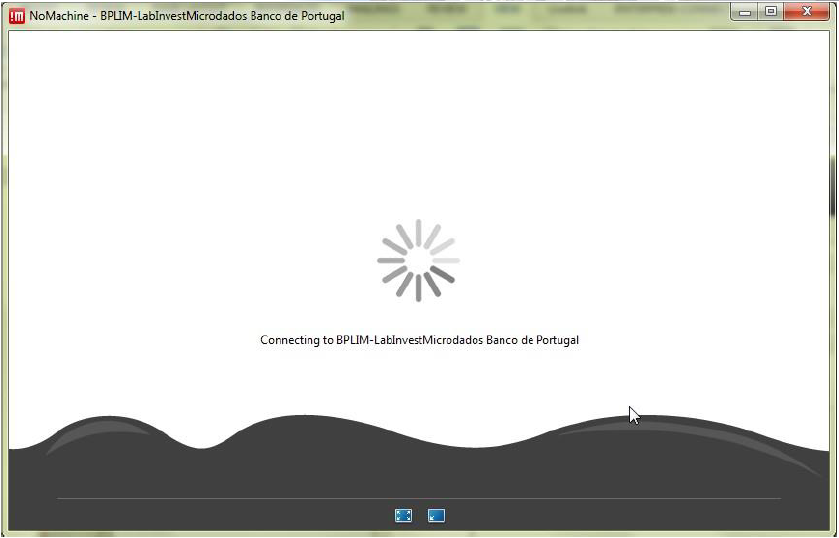
\includegraphics[width=4.72441in,height=3.02971in]{./media/image36.png}

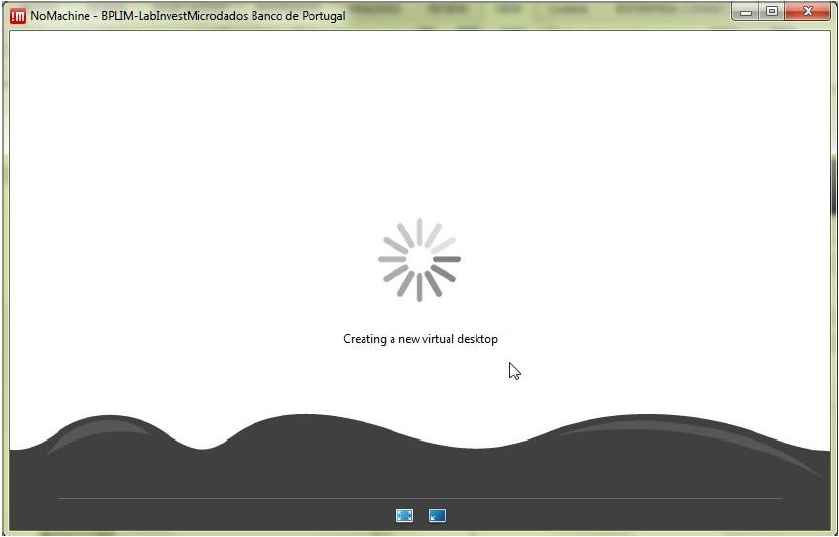
\includegraphics[width=4.72441in,height=3.02389in]{./media/image37.png}

Once logged in and with access to a KDE session, click on the upper
right corner of the KDE desktop, as shown below, to access the menu
and then expand the screen as exemplified for greater ease of use.

\textbf{Step 5.12}: You should see the following screen.

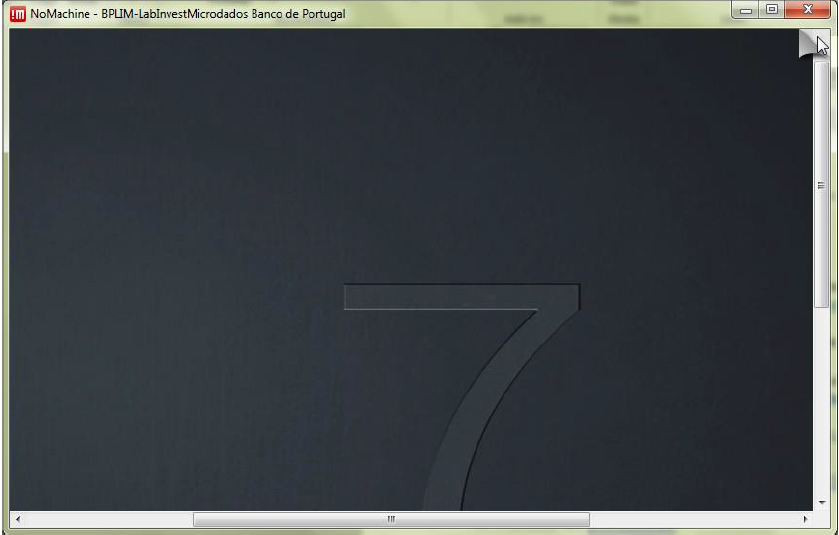
\includegraphics[width=4.72441in,height=3.01274in]{./media/image38.png}

\textbf{Step 5.13}: Click `Display'

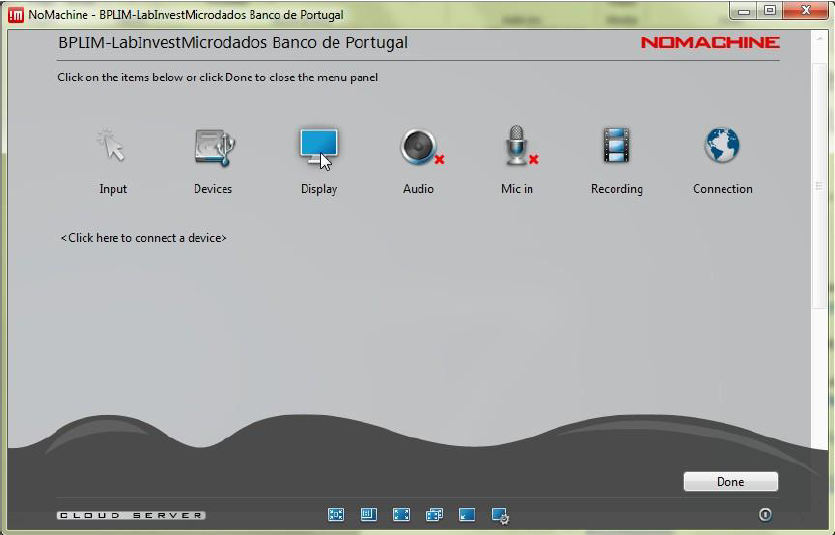
\includegraphics[width=4.72441in,height=3.0268in]{./media/image39.png}

\textbf{Step 5.14}: Click `Fit to window' and click `Done'

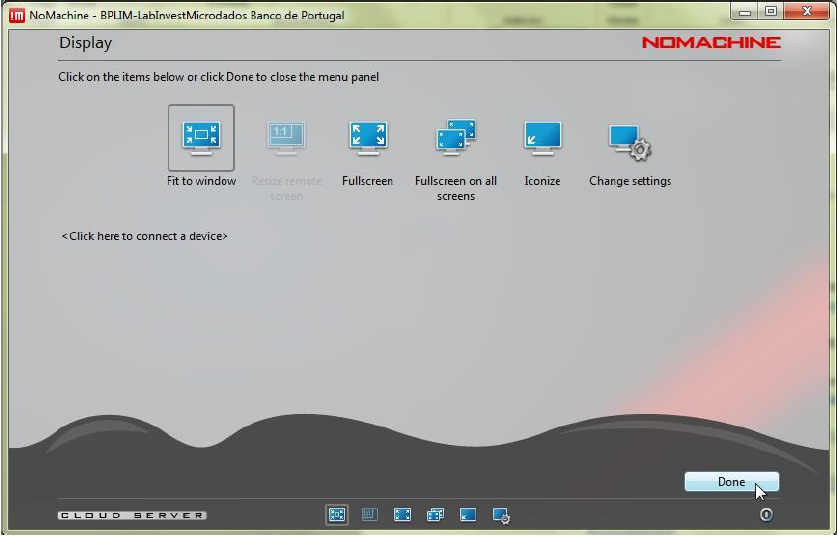
\includegraphics[width=4.72441in,height=3.02195in]{./media/image40.png}
\end{quote}

\hypertarget{appendix-5-browser-access}{%
\section{\texorpdfstring{{Appendix 5 -- Browser access}}{Appendix 5 -- Browser access}}\label{appendix-5-browser-access}}

\begin{quote}
Use a browser (recommended Chrome, Firefox, Opera or Safari) and go to
\url{https://bplim.bportugal.pt:4443}
\end{quote}

Configuring browser access

\begin{quote}
To a large extent the configuration of the access via browser is
similar to the configuration through the client NoMachine. However,
the features and performance are lower than the ``NoMachine client
access''.

In case you are using a Portuguese Keyboard, note that the keyboard
has to be set to Portuguese, as shown below, and even then some
characters may have to be specified on the virtual keyboard (depending
on the browser used). Please confirm the configuration of characters
on your keyboard.

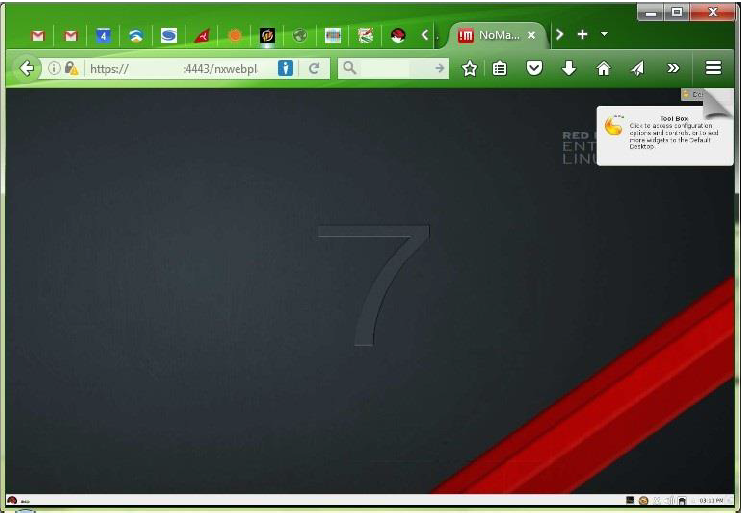
\includegraphics[width=4.72441in,height=3.26627in]{./media/image41.png}

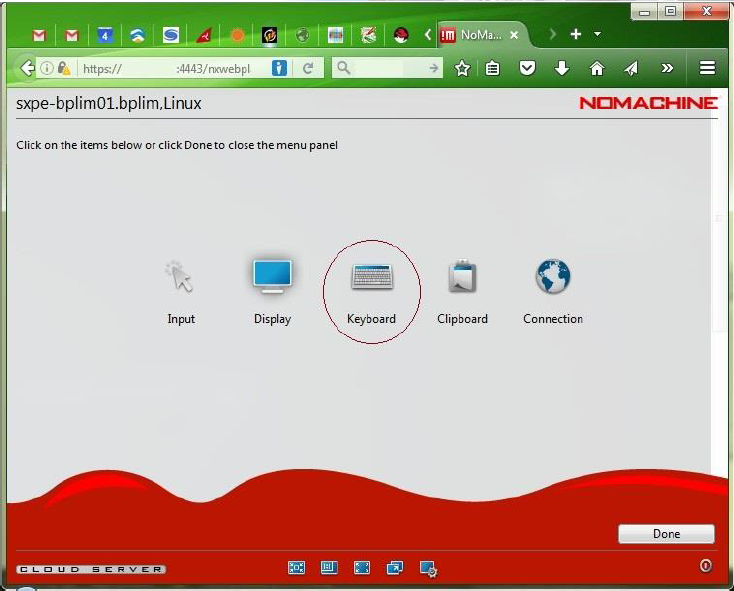
\includegraphics[width=4.72441in,height=3.80386in]{./media/image42.png}

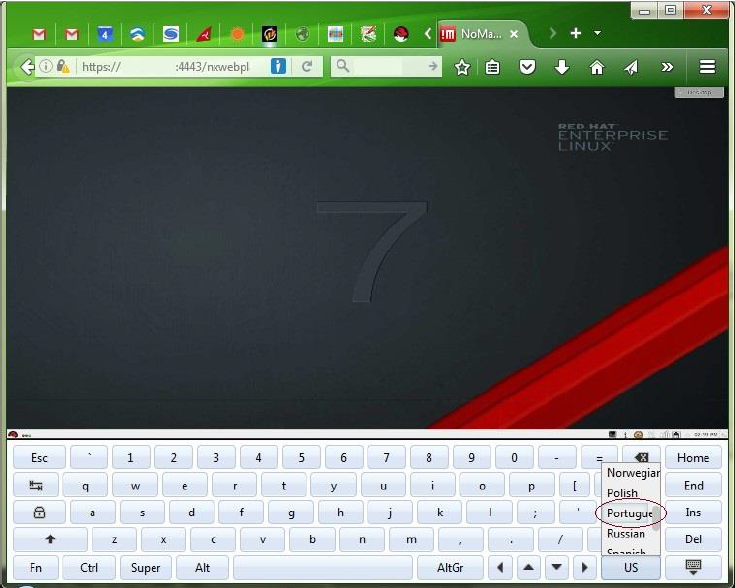
\includegraphics[width=4.72441in,height=3.77962in]{./media/image43.png}

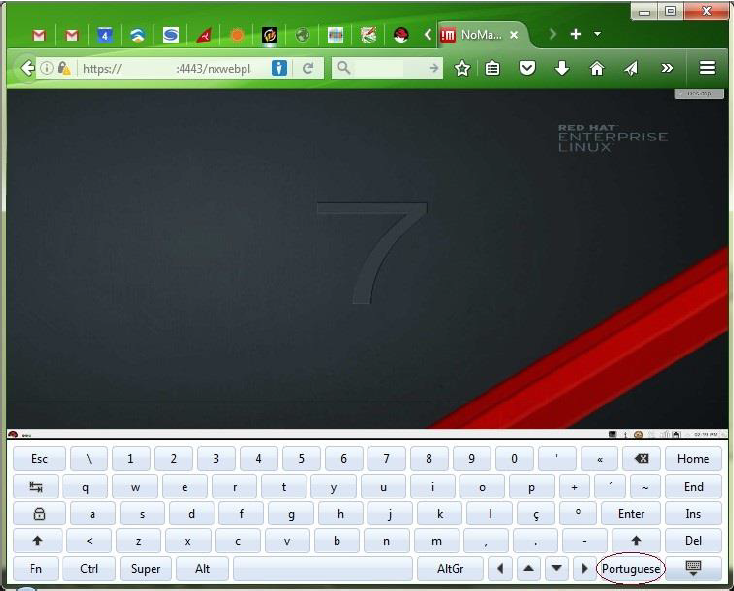
\includegraphics[width=4.72441in,height=3.80386in]{./media/image44.png}
\end{quote}

\hypertarget{appendix-6-frequently-asked-questions}{%
\section{\texorpdfstring{{Appendix 6 -- Frequently Asked Questions}}{Appendix 6 -- Frequently Asked Questions}}\label{appendix-6-frequently-asked-questions}}

\begin{enumerate}
\def\labelenumi{\arabic{enumi}.}
\tightlist
\item
  After the login in ``\url{https://webfa.bportugal.pt}'' I am not able to
  dowload NoMachine's setup file
\end{enumerate}

It may occur that a firewall is preventing the download. We have
verified such problem in some Universities and Governmental services.
Please try the download outside the firewall

\begin{enumerate}
\def\labelenumi{\arabic{enumi}.}
\setcounter{enumi}{1}
\tightlist
\item
  Mac users are not able to install NoMachine, receiving the following
  message
\end{enumerate}

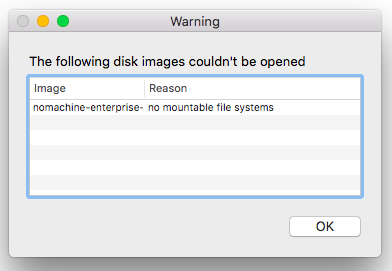
\includegraphics[width=2.16535in,height=1.49697in]{./media/image45.png}

Please check if your Mac OSX is updated. Temporary solution: download
NoMachine Enterprise Client from the official website, and run the
installation file:

\url{https://www.nomachine.com/download-enterprise/\#NoMachine-Enterprise-Client}

\begin{enumerate}
\def\labelenumi{\arabic{enumi}.}
\setcounter{enumi}{2}
\tightlist
\item
  NoMachine authentication failure
\end{enumerate}

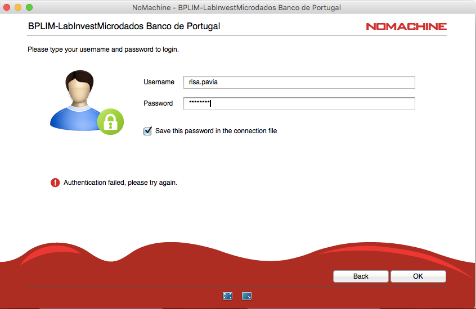
\includegraphics[width=2.16535in,height=1.40773in]{./media/image46.png}

\begin{itemize}
\item
  We have observed that some users who change their password within
  ``\url{https://webfa.bportugal.pt}'' later are not able to login within
  NoMachine (error message shown in the image above). In some cases it
  occurs due to a different keyboard layout. For example, if you have
  a Portuguese keyboard, but the website assumed a US keyboard, and
  your password contains a symbol like `ç', than you will get a ``wrong
  password'' message. Please check the keyboard layout that is active
  when you type the password. Alternatively, change the password after
  the first login with NoMachine. Use linux's command `passwd'.
\item
  Login fails and the system shows the message: "Could not connect to
  the server. Error is 138: Connection is timed out" Please check if
  your network has a strict firewall; e.g., some researchers are not
  able to reach BPLIM's server within their University network. Please
  check if in a different location, like at home, the connection
  works.
\end{itemize}

\begin{enumerate}
\def\labelenumi{\arabic{enumi}.}
\setcounter{enumi}{3}
\tightlist
\item
  User pressed `Lock' instead of `Log out' and the unlock/password
  does not work:
\end{enumerate}

\begin{itemize}
\item
  Check if the keyboard settings are correct (e.g., PT or UK)
\item
  Close the `NoMachine' connection and start a new one. Before the
  last step -before the 'Login'- right click and choose `Logout'.
  Double-click for the new connection
\end{itemize}

\begin{enumerate}
\def\labelenumi{\arabic{enumi}.}
\setcounter{enumi}{4}
\tightlist
\item
  ``Cannot see the screen in NoMachine'' (see image below)
\end{enumerate}

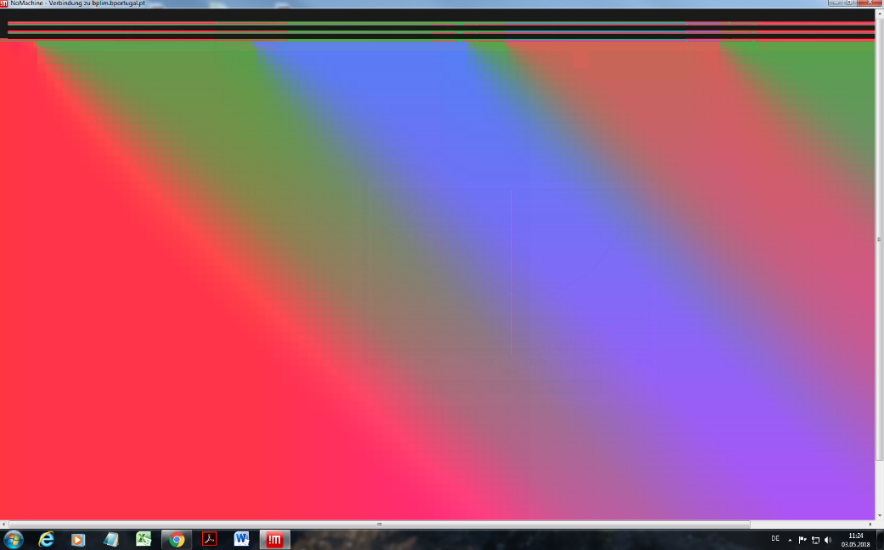
\includegraphics[width=4.01667in,height=2.49995in]{./media/image47.png}

\begin{enumerate}
\def\labelenumi{\arabic{enumi}.}
\setcounter{enumi}{4}
\tightlist
\item
  {OPTION A}: move your mouse on top the upper right
  corner of NoMachine, you should see a ``folded like sheet'',
  left-click your mouse, go to `Display', `Change settings', and click
  in `Disable client side hardware decoding'
\end{enumerate}

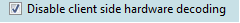
\includegraphics[width=1.56522in,height=0.15in]{./media/image48.png}

\begin{enumerate}
\def\labelenumi{\arabic{enumi}.}
\setcounter{enumi}{5}
\tightlist
\item
  {OPTION B}: Close the `NoMachine' connection and start a
  new one. Before the last step -before the 'Login'- right click and
  choose `Logout'. Double-click for the new connection
\end{enumerate}

\hypertarget{central-de-balancos-central-balance-sheet-database---harmonized-panel-data}{%
\chapter{Central de Balanços (Central Balance Sheet Database) - Harmonized Panel Data}\label{central-de-balancos-central-balance-sheet-database---harmonized-panel-data}}

\hypertarget{data-manual}{%
\section{Data manual}\label{data-manual}}

\textbf{Abstract}: In 2010, the national accounting standards underwent some changes, and \emph{Plano Oficial de Contabilidade} (POC, National Plan of Accounts) was replaced by \emph{Sistema de Normalização Contabilística} (SNC, Accounting Normalization System). This had an impact on the base information in the Central Balance Sheet Database. This manual describes the panel data of \emph{Central de Balanços} with harmonized variables over time available at BPLIM.

\hypertarget{table-of-contents}{%
\chapter{Table of contents}\label{table-of-contents}}

\begin{enumerate}
\def\labelenumi{\arabic{enumi}.}
\tightlist
\item
  \protect\hyperlink{general-information}{General Information}
\item
  \protect\hyperlink{geographical-coverage}{Geographical Coverage}
\item
  \protect\hyperlink{population}{Population}
\item
  \protect\hyperlink{methodology}{Methodology}
\item
  \protect\hyperlink{description-of-files}{Description of files}
\item
  \protect\hyperlink{description-of-variables}{Description of variables}

  \begin{enumerate}
  \def\labelenumii{\arabic{enumii}.}
  \tightlist
  \item
    \protect\hyperlink{a.-general-information-file-cover-sheet}{General Information File (Cover Sheet)}
  \item
    \protect\hyperlink{b.-economic-and-financial-information-file}{Economic and Financial Information File}
  \item
    \protect\hyperlink{c.-employment-information-file}{Employment Information File}
  \item
    \protect\hyperlink{d.-trade-information-per-market-file}{Trade Information per Market File}
  \item
    \protect\hyperlink{e.-economic-and-financial-indicators}{Economic and Financial Indicators File}
  \end{enumerate}
\item
  \protect\hyperlink{basic-descriptive-statistics}{Basic Descriptive Statistics}
\item
  \protect\hyperlink{citation-of-this-dataset}{Citation of this dataset}
\item
  \protect\hyperlink{auxiliary-files}{Auxiliary Files}
\item
  \protect\hyperlink{references}{References}
\item
  \protect\hyperlink{appendix}{Appendix}
\end{enumerate}

\hypertarget{general-information}{%
\chapter{General Information}\label{general-information}}

\begin{quote}
\texttt{Data\ Type}: Longitudinal Data
\end{quote}

\begin{quote}
\texttt{Units\ of\ Analysis}: Firms
\end{quote}

\begin{quote}
\texttt{Frequency}: Annual
\end{quote}

\begin{quote}
\texttt{Start\ Date}: 2006
\end{quote}

\begin{quote}
\texttt{Most\ recent\ year}: 2016
\end{quote}

\begin{quote}
\texttt{Reference\ date}: The data reports to the fiscal period declared by the firm. For most cases, the fiscal period coincides with the civil year. For those firms with fiscal period different than the civil year, the reference year is the one covering most of the days of the fiscal period.
\end{quote}

\begin{quote}
\texttt{Data\ Organization}: Data is organized in four files:
\end{quote}

\begin{itemize}
\tightlist
\item
  General Information on the firm (Cover Sheet),
\item
  Economic and Financial Information (Balance Sheet and Profit and Loss Statements),
\item
  Employment Information,
\item
  Trade Information per Market.
\end{itemize}

In all files each row corresponds to one firm in a given year. All files are available in Stata format, version 15.

\begin{quote}
\texttt{Version\ of\ the\ Data}: The data made available by BPLIM corresponds to a data freeze at a certain time of the year.\footnote{For more information, see the manual on the Annual Data of Central Balance Sheet Database.} Therefore, all files contain the information as reported in the extraction date. The most recent update of the data occurred in June 2018.
\end{quote}

\begin{quote}
\texttt{Languages\ Available}: Variable labels and value labels are available in Portuguese and for most of the variables also in English. \footnote{To see the labels in English type the following command line in Stata: `label language en'.}
\end{quote}

\begin{quote}
\texttt{Related\ Datasets}: This product is built based on the information from Central Balance Sheet Database.
\end{quote}

\hypertarget{geographical-coverage}{%
\chapter{Geographical Coverage}\label{geographical-coverage}}

The data refers to firms located in the Mainland Portugal and Autonomous Regions -- Azores and Madeira.

\hypertarget{population}{%
\chapter{Population}\label{population}}

The population of the panel dataset of \emph{Central de Balanços} is the same as in the annual data, i.e.~the population of all Portuguese non-financial corporations. For more information, please see the manual on \href{../../CB/Jun2018/Pack_CB_Empresas_Jun18/manual_CB_Jun2018.html}{\emph{Central Balance Sheet Database - Annual Data}}.

\hypertarget{methodology}{%
\chapter{Methodology}\label{methodology}}

Central Balance Sheet Database provides economic and financial information on Portuguese non-financial corporations. The data is collected through \emph{Informação Empresarial Simplicada} (IES) since 2006. In 2010, the national accounting standards underwent some changes, and \emph{Plano Oficial de Contabilidade} (POC, National Plan of Accounts) was replaced by \emph{Sistema de Normalização Contabilística} (SNC, Accounting Normalization System), which is closer to the International Accounting Standards (IAS) and International Financial Reporting Standards (IFRS). This had an impact on the base information in the Central Balance Sheet Database (Banco de Portugal, 2014).

\includegraphics{./media/accounting_years.png}

With the introduction of SNC, some accounting items were simply redenominated, some were aggregated or disaggregated, and others have no correspondence at all in the old accounting system. The Interest income (VF16150) and Net non-current assets held for sale (VF16035) are some examples of variables that are not reported in the financial statements written according to POC. Also, the asset items in POC accounting system were reported in gross terms and the amortizations and adjustments were reported separately for each item of the Balance Sheet. The financial statement written according to SNC does not have a separate item for depreciations as POC did and all variables are being reported in net terms.
Finally, SNC introduced different reporting standards for firms with different sizes. After 2010, Micro-Entities and Small-sized Entities \footnote{A Micro-Entity is defined as a firm that falls below in at least two of the following criteria at the balance sheet date: i) total assets equal to 500.000 euros; ii) net turnover equal to 500.000 euros; or iii) average number of employees equal to 5. Small-sized Entities are firms satisfying at least two of the following conditions: i) total assets below 500.000 euros; ii) total gross sales and other income lower than 1.000.000 euros or; iii) average number of employees less than 20. For more details please check the manual on \href{../../CB/Jun2018/Pack_CB_Empresas_Jun18/manual_CB_Jun2018.html}{\emph{Central Balance Sheet Database - Annual Data}}.} were required to report a lower number of variables.

In this section, we describe the procedure to compute the harmonized variables available in the panel data of Central Balance Sheet Database. For a complete account on how each variable made available in the panel was computed, check the \protect\hyperlink{description-of-variables}{Description of Variables}.
All the calculations are done based on the annual files of \emph{Central de Balanços}. Therefore, the number of firms and the time period available are the same as in the annual files. The panel dataset is updated once per year around the month of June, at the same time as the annual data of \emph{Central de Balanços}. The most recent extraction occurred in June 2018.

Some variables had to be aggregated to guarantee the comparability before and after 2010. Besides, the harmonized variables can only be calculated if their components are reported for all entities according to the reporting standards adopted by the firm. Therefore, the panel dataset contains a lower number of variables than those included in the annual files.
Currently we make available approximately 60 harmonized variables on the Balance Sheet and Profit and Loss Statement. In the Employment Information file, we make available 18 variables and in the Trade Information per market file, 12 variables are available. All variables in the Cover Sheet File are available given that this type of information were not affected by the accounting standards.

Table 1 -- Number of Harmonized Variables by type of information

\begin{longtable}[]{@{}lcc@{}}
\toprule
Type of Information & Number of Harmonized Variables & Time Period\tabularnewline
\midrule
\endhead
General Information (Cover sheet) File & 23 & 2006-2016\tabularnewline
Economic and Financial Information File & 59 & 2006-2016\tabularnewline
Employment Information File & 18 & 2006-2016\tabularnewline
Trade Information per Market File & 12 & 2006-2016\tabularnewline
\bottomrule
\end{longtable}

The harmonization procedure is different for each file described in Table 1. While the information in the Cover sheet did not suffer any significant change with the introduction of SNC, the harmonization of the Economic and Financial Information is not a straightforward task. Therefore, we classified the harmonization methodology in three different categories:

\begin{itemize}
\item
  \textbf{Type 1}: covers the information unaffected by the change in the accounting system, which includes the Cover Sheet File. In this case, we simply append the annual datasets. The name of the variables remain the same since no change on the original data was undertaken.
\item
  \textbf{Type 2}: covers the information that was directly affected by the change in the accounting system, i.e., the Economic and Financial Information and Trade Information per Market. It also includes the Employment Information because the variables are collected through different tables in IES and have different denominations under POC and SNC accounting systems.
  For this type of files, we rely on the definition of the variables under the current accounting system (SNC) and compute a formula using the POC items needed to ensure the comparability over time.
  For example, the procedure to compute the item Turnover (D001) is illustrated below:
\end{itemize}

\begin{longtable}[]{@{}cccccccc@{}}
\toprule
\endhead
\textbf{ano} & \textbf{tina} & planocont & VF03045 & VF03046 & VF03047 & VF16132 & \textbf{D001}\tabularnewline
\textbf{2006} & \textbf{500000000} & POC & . & . & . & . & \textbf{0}\tabularnewline
\textbf{2007} & \textbf{500000000} & POC & 100 & 100 & 100 & . & \textbf{300}\tabularnewline
\textbf{2008} & \textbf{500000000} & POC & 100 & 100 & . & . & \textbf{200}\tabularnewline
\textbf{2009} & \textbf{500000000} & POC & 100 & 100 & 100 & . & \textbf{300}\tabularnewline
\textbf{2010} & \textbf{500000000} & SNC & . & . & . & 100 & \textbf{100}\tabularnewline
\textbf{2011} & \textbf{500000000} & SNC & . & . & . & 100 & \textbf{100}\tabularnewline
\textbf{2012} & \textbf{500000000} & SNC & . & . & . & 100 & \textbf{100}\tabularnewline
\textbf{2013} & \textbf{500000000} & SNC & . & . & . & 100 & \textbf{100}\tabularnewline
\textbf{2014} & \textbf{500000000} & SNC & . & . & . & 100 & \textbf{100}\tabularnewline
\textbf{2015} & \textbf{500000000} & SNC & . & . & . & 100 & \textbf{100}\tabularnewline
\textbf{2016} & \textbf{500000000} & SNC & . & . & . & 100 & \textbf{100}\tabularnewline
\bottomrule
\end{longtable}

The SNC variable - VF16132 (Turnover) - corresponds to the sum of the variables VF03045, VF03046 and VF03047 in the POC accounting system. Therefore, a new harmonized variable is computed - D001 - using these auxiliary variables. After calculating the harmonized variable, the auxiliary variables are dropped and only the variables in bold are kept in the dataset.
All missing values in the auxiliary variables are treated as zeros. The report of IES is mandatory for all firms that are required to send the financial statements to the Ministry of Finance. Therefore, all items have to be completed in a consistent manner so that the firm is able to submit the declaration. Therefore, the real value of a specific variable is assumed to be zero if it is not reported.
The naming convention for Balance Sheet variables in the panel data is B(L)xxx, for Profit and Loss Statement is D(L)xxx, for Employment Information is Exxx and for Trade Information per Market is MGxxx.

After identifying all variables that can be potentially included in the panel dataset, we produced and analyzed technical reports on each variable. Namely, we did the following checks to ensure the compatibility of the panel variables over time:

\begin{enumerate}
\def\labelenumi{\arabic{enumi}.}
\tightlist
\item
  analyze the evolution of the mean and medium values of the relative changes over time. \footnote{The relative changes are defined as the difference between the value of the variable observed in year t minus the value observed in the previous year. Relative changes are computed with respect to the average of year t and t-1 and are measured in percentage.} We try to identify whether there is any discontinuity in 2010, the first year in which most of the firms reported under \emph{Sistema de Normalização Contabilística}.\footnote{In 2010 some declarations were reported according to \emph{Plano Oficial de Contas}. This situation occurs mostly for declarations sent in the cessation period and before or after the firms adopts a special fiscal period - a fiscal period different from calendar year.}
\item
  check whether abnormal relative changes (relative changes above 100\%) are found more often in the transition to the new accounting system.
\item
  decomposition of the yearly variation of the total value of each variable due to the expansion and contraction of incumbents and the entry and exit of firms.
\item
  regression of each variable on time dummies to detect any structural change in the variable after 2010.
\end{enumerate}

The link to the report on each variable is available in the section \protect\hyperlink{description-of-variables}{Description of Variables}.
The harmonization procedure tries to ensure the compatibility of the variable over time as much as possible. However, as one can see in the variable reports, some harmonized variables show a clear discontinuity in 2010.

We also produce a \href{./Auxiliary\%20Files/technical_reports/CONTAS_MG_checks.pdf}{report} checking whether the sum of disaggregated variables corresponds to the aggregated variables.

\begin{itemize}
\tightlist
\item
  \textbf{Type 3}: covers the Economic and Financial Indicators files containing information affected by the change in the accounting system. The information on this file is calculated using the variables available in the Economic and Financial Information File. We provide a Stata ado file to compute all the economic and financial indicators that are possible to harmonize over time given the information available in the panel dataset. By adopting this procedure, the size of the dataset is minimized. All indicators variables calculated by this ado are denominated Rxxx.
\end{itemize}

\hypertarget{description-of-files}{%
\chapter{Description of Files}\label{description-of-files}}

Similarly to the annual data files, the panel data of \emph{Central de Balanços} is organized in four files. Each file provides a different type of information, namely:

\begin{longtable}[]{@{}ll@{}}
\toprule
\begin{minipage}[b]{0.35\columnwidth}\raggedright
Type of Information\strut
\end{minipage} & \begin{minipage}[b]{0.59\columnwidth}\raggedright
File Name\strut
\end{minipage}\tabularnewline
\midrule
\endhead
\begin{minipage}[t]{0.35\columnwidth}\raggedright
\textbf{A. General Information (Cover sheet)}\strut
\end{minipage} & \begin{minipage}[t]{0.59\columnwidth}\raggedright
CB\_A\_FRM\_PanelyyYYeeee\_ROSTO\_V01.dta\strut
\end{minipage}\tabularnewline
\begin{minipage}[t]{0.35\columnwidth}\raggedright
\textbf{B. Economic and Financial Information}\strut
\end{minipage} & \begin{minipage}[t]{0.59\columnwidth}\raggedright
CB\_A\_FRM\_PanelyyYYeeee\_CONTAS\_V01.dta\strut
\end{minipage}\tabularnewline
\begin{minipage}[t]{0.35\columnwidth}\raggedright
\textbf{C. Employment Information}\strut
\end{minipage} & \begin{minipage}[t]{0.59\columnwidth}\raggedright
CB\_A\_FRM\_PanelyyYYeeee\_PESSOAL\_V01.dta\strut
\end{minipage}\tabularnewline
\begin{minipage}[t]{0.35\columnwidth}\raggedright
\textbf{D. Trade Information per Market}\strut
\end{minipage} & \begin{minipage}[t]{0.59\columnwidth}\raggedright
CB\_A\_FRM\_PanelyyYYeeee\_MG\_V01.dta\strut
\end{minipage}\tabularnewline
\bottomrule
\end{longtable}

Where \emph{A} stands for Anonymized and \emph{yy} corresponds to the first year available and \emph{YY} corresponds to most recent year available. \emph{eee} reports the extraction date.

All files contain a unique firm identifier (\emph{tina}) and a reference year (\emph{ano}) allowing the matching of the different types of information by firm. Whenever possible, labels and value labels were attributed to all categorical variables. All data sets are anonymized.

\hypertarget{description-of-variables}{%
\chapter{Description of Variables}\label{description-of-variables}}

\hypertarget{a.-general-information-file-cover-sheet}{%
\section{A. General Information File (Cover Sheet)}\label{a.-general-information-file-cover-sheet}}

The information reported in this file was not affected by the change in the accounting system. Therefore, the panel dataset includes all the variables available in the annual data files.

\hypertarget{a1.-identifiers}{%
\subsection{A1. Identifiers}\label{a1.-identifiers}}

\texttt{Firm\ identifier} (\emph{tina}) -- Unique identifier that enables tracking the legal entity firm over time. \emph{tina} is the anonymized tax identification number. The first digit of the tax identification number contains information on the type of corporation and legal form. Therefore, this first digit is preserved in \emph{tina}.

\texttt{Reference\ year\ of\ the\ data} (\emph{ano}) -- Reference year of the data.

\hypertarget{a2.-other-variables}{%
\subsection{A2. Other variables}\label{a2.-other-variables}}

All the variables available in the annual datasets are also available in the panel data of Central Balance Sheet Database. For a full description of these variables please check the manual on \href{../../CB/Jun2018/Pack_CB_Empresas_Jun18/manual_CB_Jun2018.html}{\emph{Central Balance Sheet Database - Annual Data}} or the auxiliary file \href{./Auxiliary\%20Files/variables_description/var_rosto.html}{var\_rosto.html}.

The variables reporting the accounting system (\emph{planocont}) and the accounting standards (\emph{regime}) under which the firm is reporting information are kept in the panel dataset. These variables do not have any interpretation given that all the economic and financial variables included in the panel dataset are harmonized over time. They are kept in the dataset because they may be useful in case one wants to calculate additional variables not provided by BPLIM.

\hypertarget{b.-economic-and-financial-information-file}{%
\section{B. Economic and Financial Information File}\label{b.-economic-and-financial-information-file}}

This file provides a set of balance sheet and profit and loss statement variables harmonized over time. For a full account of the SNC items included in the definition of the harmonized variable see the auxiliary file \href{./Auxiliary\%20Files/variables_description/contas_snc_items.html}{contas\_snc\_items.html}.

\hypertarget{b1.-identifiers}{%
\subsection{B1. Identifiers}\label{b1.-identifiers}}

\texttt{Firm\ identifier} (\emph{tina}) -- Unique identifier that enables tracking the legal entity firm over time. \emph{tina} is the anonymized tax identification number.

\texttt{Reference\ year\ of\ the\ data} (\emph{ano}) -- Reference year of the data.

\hypertarget{b2.-balance-sheet-variables}{%
\subsection{B2. Balance Sheet Variables}\label{b2.-balance-sheet-variables}}

\hypertarget{assets}{%
\subsection{Assets}\label{assets}}

\begin{longtable}[]{@{}cllccc@{}}
\toprule
\begin{minipage}[b]{0.08\columnwidth}\centering
Variable\strut
\end{minipage} & \begin{minipage}[b]{0.20\columnwidth}\raggedright
Variable description\strut
\end{minipage} & \begin{minipage}[b]{0.16\columnwidth}\raggedright
Definition\strut
\end{minipage} & \begin{minipage}[b]{0.09\columnwidth}\centering
SNC Variable\strut
\end{minipage} & \begin{minipage}[b]{0.15\columnwidth}\centering
Formula in POC\strut
\end{minipage} & \begin{minipage}[b]{0.16\columnwidth}\centering
Variable Report\strut
\end{minipage}\tabularnewline
\midrule
\endhead
\begin{minipage}[t]{0.08\columnwidth}\centering
B001\strut
\end{minipage} & \begin{minipage}[t]{0.20\columnwidth}\raggedright
\textbf{Total Assets (QS)}\strut
\end{minipage} & \begin{minipage}[t]{0.16\columnwidth}\raggedright
Total non-current assets; Total current assets\strut
\end{minipage} & \begin{minipage}[t]{0.09\columnwidth}\centering
VF15991\strut
\end{minipage} & \begin{minipage}[t]{0.15\columnwidth}\centering
\protect\hyperlink{b001---formula-in-poc}{Formula in POC}\strut
\end{minipage} & \begin{minipage}[t]{0.16\columnwidth}\centering
\href{./Auxiliary\%20Files/technical_reports/variable_report/B001(!).pdf}{Report - B001}\strut
\end{minipage}\tabularnewline
\begin{minipage}[t]{0.08\columnwidth}\centering
B004\strut
\end{minipage} & \begin{minipage}[t]{0.20\columnwidth}\raggedright
\textgreater{} Total non-current assets (QS)\strut
\end{minipage} & \begin{minipage}[t]{0.16\columnwidth}\raggedright
Fixed tangible assets and intangible assets; Financial investments; Remaining non-current assets\strut
\end{minipage} & \begin{minipage}[t]{0.09\columnwidth}\centering
VF15994\strut
\end{minipage} & \begin{minipage}[t]{0.15\columnwidth}\centering
\protect\hyperlink{b004---formula-in-poc}{Formula in POC}\strut
\end{minipage} & \begin{minipage}[t]{0.16\columnwidth}\centering
\href{./Auxiliary\%20Files/technical_reports/variable_report/B004(!).pdf}{Report - B004}\strut
\end{minipage}\tabularnewline
\begin{minipage}[t]{0.08\columnwidth}\centering
B005\strut
\end{minipage} & \begin{minipage}[t]{0.20\columnwidth}\raggedright
\textgreater{} \textgreater{} Fixed tangible assets and intangible assets\strut
\end{minipage} & \begin{minipage}[t]{0.16\columnwidth}\raggedright
Intangible assets (including Goodwill); Land and buildings; Basic equipment; Other fixed assets; Payments on account of fixed assets\strut
\end{minipage} & \begin{minipage}[t]{0.09\columnwidth}\centering
VF15995\strut
\end{minipage} & \begin{minipage}[t]{0.15\columnwidth}\centering
\protect\hyperlink{b005---formula-in-poc}{Formula in POC}\strut
\end{minipage} & \begin{minipage}[t]{0.16\columnwidth}\centering
\href{./Auxiliary\%20Files/technical_reports/variable_report/B005.pdf}{Report - B005}\strut
\end{minipage}\tabularnewline
\begin{minipage}[t]{0.08\columnwidth}\centering
B012\strut
\end{minipage} & \begin{minipage}[t]{0.20\columnwidth}\raggedright
\textgreater{} \textgreater{} \textgreater{} Fixed tangible assets\strut
\end{minipage} & \begin{minipage}[t]{0.16\columnwidth}\raggedright
Land and buildings; Basic equipment; Other fixed assets; Payments on account of fixed assets \footnotemark{}\strut
\end{minipage}
\footnotetext{With the introduction of SNC some components that were previously classified as fixed tangible assets were reallocated to intangible assets to accommodate international standards. An example is highway concessions which were considered as tangible assets in POC and were reclassified as intangible assets in SNC.} & \begin{minipage}[t]{0.09\columnwidth}\centering
VF16002\strut
\end{minipage} & \begin{minipage}[t]{0.15\columnwidth}\centering
\protect\hyperlink{b012---formula-in-poc}{Formula in POC}\strut
\end{minipage} & \begin{minipage}[t]{0.16\columnwidth}\centering
\href{./Auxiliary\%20Files/technical_reports/variable_report/B012.pdf}{Report - B012}\strut
\end{minipage}\tabularnewline
\begin{minipage}[t]{0.08\columnwidth}\centering
B025\strut
\end{minipage} & \begin{minipage}[t]{0.20\columnwidth}\raggedright
\textgreater{} \textgreater{} Financial investments\strut
\end{minipage} & \begin{minipage}[t]{0.16\columnwidth}\raggedright
Investments in subsidiary and associated companies; Financial investments (excepting investments in subsidiary and associated companies\strut
\end{minipage} & \begin{minipage}[t]{0.09\columnwidth}\centering
VF16015\strut
\end{minipage} & \begin{minipage}[t]{0.15\columnwidth}\centering
\protect\hyperlink{b025---formula-in-poc}{Formula in POC}\strut
\end{minipage} & \begin{minipage}[t]{0.16\columnwidth}\centering
\href{./Auxiliary\%20Files/technical_reports/variable_report/B025(!).pdf}{Report - B025}\strut
\end{minipage}\tabularnewline
\begin{minipage}[t]{0.08\columnwidth}\centering
B158\strut
\end{minipage} & \begin{minipage}[t]{0.20\columnwidth}\raggedright
\textgreater{} \textgreater{} Non-current assets - Remaining non-current assets\strut
\end{minipage} & \begin{minipage}[t]{0.16\columnwidth}\raggedright
Shareholders / partners; Deferred tax assets\strut
\end{minipage} & \begin{minipage}[t]{0.09\columnwidth}\centering
VF18510\strut
\end{minipage} & \begin{minipage}[t]{0.15\columnwidth}\centering
\protect\hyperlink{b158---formula-in-poc}{Formula in POC}\strut
\end{minipage} & \begin{minipage}[t]{0.16\columnwidth}\centering
\href{./Auxiliary\%20Files/technical_reports/variable_report/B158.pdf}{Report - B158}\strut
\end{minipage}\tabularnewline
\begin{minipage}[t]{0.08\columnwidth}\centering
B029\strut
\end{minipage} & \begin{minipage}[t]{0.20\columnwidth}\raggedright
\textgreater{} Total Current assets (QS)\strut
\end{minipage} & \begin{minipage}[t]{0.16\columnwidth}\raggedright
Inventories and biological assets; Customers; Remaining current assets; Cash and bank deposits; Non-current assets held for sale \footnotemark{}\strut
\end{minipage}
\footnotetext{This variable has no match in \emph{Plano Oficial de Contas}.} & \begin{minipage}[t]{0.09\columnwidth}\centering
VF16019\strut
\end{minipage} & \begin{minipage}[t]{0.15\columnwidth}\centering
\protect\hyperlink{b029---formula-in-poc}{Formula in POC}\strut
\end{minipage} & \begin{minipage}[t]{0.16\columnwidth}\centering
\href{./Auxiliary\%20Files/technical_reports/variable_report/B029(!).pdf}{Report - B029}\strut
\end{minipage}\tabularnewline
\begin{minipage}[t]{0.08\columnwidth}\centering
B032\strut
\end{minipage} & \begin{minipage}[t]{0.20\columnwidth}\raggedright
\textgreater{} \textgreater{} Current assets - Inventories and biological assets\strut
\end{minipage} & \begin{minipage}[t]{0.16\columnwidth}\raggedright
Raw and subsidiary materials and consumables; Advances from customers; Inventories (excepting Raw and subsidiary materials and consumables)\strut
\end{minipage} & \begin{minipage}[t]{0.09\columnwidth}\centering
VF16022\strut
\end{minipage} & \begin{minipage}[t]{0.15\columnwidth}\centering
\protect\hyperlink{b032---formula-in-poc}{Formula in POC}\strut
\end{minipage} & \begin{minipage}[t]{0.16\columnwidth}\centering
\href{./Auxiliary\%20Files/technical_reports/variable_report/B032(!).pdf}{Report - B032}\strut
\end{minipage}\tabularnewline
\begin{minipage}[t]{0.08\columnwidth}\centering
B041\strut
\end{minipage} & \begin{minipage}[t]{0.20\columnwidth}\raggedright
\textgreater{} \textgreater{} Current assets - Customers\strut
\end{minipage} & \begin{minipage}[t]{0.16\columnwidth}\raggedright
\strut
\end{minipage} & \begin{minipage}[t]{0.09\columnwidth}\centering
VF16031\strut
\end{minipage} & \begin{minipage}[t]{0.15\columnwidth}\centering
\protect\hyperlink{b041---formula-in-poc}{Formula in POC}\strut
\end{minipage} & \begin{minipage}[t]{0.16\columnwidth}\centering
\href{./Auxiliary\%20Files/technical_reports/variable_report/B041(!).pdf}{Report - B041}\strut
\end{minipage}\tabularnewline
\begin{minipage}[t]{0.08\columnwidth}\centering
B049\strut
\end{minipage} & \begin{minipage}[t]{0.20\columnwidth}\raggedright
\textgreater{} \textgreater{} Current assets - Cash and bank deposits\strut
\end{minipage} & \begin{minipage}[t]{0.16\columnwidth}\raggedright
\strut
\end{minipage} & \begin{minipage}[t]{0.09\columnwidth}\centering
VF16039\strut
\end{minipage} & \begin{minipage}[t]{0.15\columnwidth}\centering
\protect\hyperlink{b049---formula-in-poc}{Formula in POC}\strut
\end{minipage} & \begin{minipage}[t]{0.16\columnwidth}\centering
\href{./Auxiliary\%20Files/technical_reports/variable_report/B049(!).pdf}{Report - B049}\strut
\end{minipage}\tabularnewline
\begin{minipage}[t]{0.08\columnwidth}\centering
B159\strut
\end{minipage} & \begin{minipage}[t]{0.20\columnwidth}\raggedright
\textgreater{} \textgreater{} Current assets - Remaining current assets\strut
\end{minipage} & \begin{minipage}[t]{0.16\columnwidth}\raggedright
Current assets - State and other public entities; Other current assets; Shareholders; Deferred expense\strut
\end{minipage} & \begin{minipage}[t]{0.09\columnwidth}\centering
VF18511\strut
\end{minipage} & \begin{minipage}[t]{0.15\columnwidth}\centering
\protect\hyperlink{b159---formula-in-poc}{Formula in POC}\strut
\end{minipage} & \begin{minipage}[t]{0.16\columnwidth}\centering
\href{./Auxiliary\%20Files/technical_reports/variable_report/B159.pdf}{Report - B159}\strut
\end{minipage}\tabularnewline
\begin{minipage}[t]{0.08\columnwidth}\centering
B042\strut
\end{minipage} & \begin{minipage}[t]{0.20\columnwidth}\raggedright
\textgreater{} \textgreater{} Current assets - State and other public entities\strut
\end{minipage} & \begin{minipage}[t]{0.16\columnwidth}\raggedright
\strut
\end{minipage} & \begin{minipage}[t]{0.09\columnwidth}\centering
VF16032\strut
\end{minipage} & \begin{minipage}[t]{0.15\columnwidth}\centering
\protect\hyperlink{b042---formula-in-poc}{Formula in POC}\strut
\end{minipage} & \begin{minipage}[t]{0.16\columnwidth}\centering
\href{./Auxiliary\%20Files/technical_reports/variable_report/B042(!).pdf}{Report - B042}\strut
\end{minipage}\tabularnewline
\bottomrule
\end{longtable}

\hypertarget{equity}{%
\subsection{Equity}\label{equity}}

\begin{longtable}[]{@{}cllccc@{}}
\toprule
\begin{minipage}[b]{0.08\columnwidth}\centering
Variable\strut
\end{minipage} & \begin{minipage}[b]{0.20\columnwidth}\raggedright
Variable description\strut
\end{minipage} & \begin{minipage}[b]{0.16\columnwidth}\raggedright
Definition\strut
\end{minipage} & \begin{minipage}[b]{0.09\columnwidth}\centering
SNC Variable\strut
\end{minipage} & \begin{minipage}[b]{0.15\columnwidth}\centering
Formula in POC\strut
\end{minipage} & \begin{minipage}[b]{0.16\columnwidth}\centering
Variable Report\strut
\end{minipage}\tabularnewline
\midrule
\endhead
\begin{minipage}[t]{0.08\columnwidth}\centering
B060\strut
\end{minipage} & \begin{minipage}[t]{0.20\columnwidth}\raggedright
\textbf{Equity and Liabilities (QS)}\strut
\end{minipage} & \begin{minipage}[t]{0.16\columnwidth}\raggedright
Equity; Liabilities\strut
\end{minipage} & \begin{minipage}[t]{0.09\columnwidth}\centering
VF16050\strut
\end{minipage} & \begin{minipage}[t]{0.15\columnwidth}\centering
\protect\hyperlink{b060---formula-in-poc}{Formula in POC}\strut
\end{minipage} & \begin{minipage}[t]{0.16\columnwidth}\centering
\href{./Auxiliary\%20Files/technical_reports/variable_report/B060(!).pdf}{Report - B060}\strut
\end{minipage}\tabularnewline
\begin{minipage}[t]{0.08\columnwidth}\centering
B061\strut
\end{minipage} & \begin{minipage}[t]{0.20\columnwidth}\raggedright
\textgreater{} \textbf{Equity (QS)}\strut
\end{minipage} & \begin{minipage}[t]{0.16\columnwidth}\raggedright
Paid-up capital; Other equity instruments; Reserves and retained earnings; Other items of equity; Net income; Interim dividends\strut
\end{minipage} & \begin{minipage}[t]{0.09\columnwidth}\centering
VF16051\strut
\end{minipage} & \begin{minipage}[t]{0.15\columnwidth}\centering
\protect\hyperlink{b061---formula-in-poc}{Formula in POC}\strut
\end{minipage} & \begin{minipage}[t]{0.16\columnwidth}\centering
\href{./Auxiliary\%20Files/technical_reports/variable_report/B061.pdf}{Report - B061}\strut
\end{minipage}\tabularnewline
\begin{minipage}[t]{0.08\columnwidth}\centering
BL005\strut
\end{minipage} & \begin{minipage}[t]{0.20\columnwidth}\raggedright
\textgreater{} \textgreater{} Legal reserves\strut
\end{minipage} & \begin{minipage}[t]{0.16\columnwidth}\raggedright
\strut
\end{minipage} & \begin{minipage}[t]{0.09\columnwidth}\centering
VF13024\strut
\end{minipage} & \begin{minipage}[t]{0.15\columnwidth}\centering
\protect\hyperlink{bl005---formula-in-poc}{Formula in POC}\strut
\end{minipage} & \begin{minipage}[t]{0.16\columnwidth}\centering
\href{./Auxiliary\%20Files/technical_reports/variable_report/BL005(!).pdf}{Report - BL005}\strut
\end{minipage}\tabularnewline
\begin{minipage}[t]{0.08\columnwidth}\centering
BL007\strut
\end{minipage} & \begin{minipage}[t]{0.20\columnwidth}\raggedright
\textgreater{} \textgreater{} Retained earnings\strut
\end{minipage} & \begin{minipage}[t]{0.16\columnwidth}\raggedright
\strut
\end{minipage} & \begin{minipage}[t]{0.09\columnwidth}\centering
VF13026\strut
\end{minipage} & \begin{minipage}[t]{0.15\columnwidth}\centering
\protect\hyperlink{bl007---formula-in-poc}{Formula in POC}\strut
\end{minipage} & \begin{minipage}[t]{0.16\columnwidth}\centering
\href{./Auxiliary\%20Files/technical_reports/variable_report/BL007.pdf}{Report - BL007}\strut
\end{minipage}\tabularnewline
\begin{minipage}[t]{0.08\columnwidth}\centering
B074\strut
\end{minipage} & \begin{minipage}[t]{0.20\columnwidth}\raggedright
\textgreater{} \textgreater{} Interim dividends\strut
\end{minipage} & \begin{minipage}[t]{0.16\columnwidth}\raggedright
\strut
\end{minipage} & \begin{minipage}[t]{0.09\columnwidth}\centering
VF16064\strut
\end{minipage} & \begin{minipage}[t]{0.15\columnwidth}\centering
\protect\hyperlink{b074---formula-in-poc}{Formula in POC}\strut
\end{minipage} & \begin{minipage}[t]{0.16\columnwidth}\centering
\href{./Auxiliary\%20Files/technical_reports/variable_report/B074(!).pdf}{Report - B074}\strut
\end{minipage}\tabularnewline
\begin{minipage}[t]{0.08\columnwidth}\centering
B143\strut
\end{minipage} & \begin{minipage}[t]{0.20\columnwidth}\raggedright
\textgreater{} \textgreater{} Subscribed capital\strut
\end{minipage} & \begin{minipage}[t]{0.16\columnwidth}\raggedright
\strut
\end{minipage} & \begin{minipage}[t]{0.09\columnwidth}\centering
VF16425\strut
\end{minipage} & \begin{minipage}[t]{0.15\columnwidth}\centering
\protect\hyperlink{b143---formula-in-poc}{Formula in POC}\strut
\end{minipage} & \begin{minipage}[t]{0.16\columnwidth}\centering
\href{./Auxiliary\%20Files/technical_reports/variable_report/B143.pdf}{Report - B143}\strut
\end{minipage}\tabularnewline
\bottomrule
\end{longtable}

\hypertarget{liabilities}{%
\subsection{Liabilities}\label{liabilities}}

\begin{longtable}[]{@{}cllccc@{}}
\toprule
\begin{minipage}[b]{0.08\columnwidth}\centering
Variable\strut
\end{minipage} & \begin{minipage}[b]{0.20\columnwidth}\raggedright
Variable description\strut
\end{minipage} & \begin{minipage}[b]{0.16\columnwidth}\raggedright
Definition\strut
\end{minipage} & \begin{minipage}[b]{0.09\columnwidth}\centering
SNC Variable\strut
\end{minipage} & \begin{minipage}[b]{0.15\columnwidth}\centering
Formula in POC\strut
\end{minipage} & \begin{minipage}[b]{0.16\columnwidth}\centering
Variable Report\strut
\end{minipage}\tabularnewline
\midrule
\endhead
\begin{minipage}[t]{0.08\columnwidth}\centering
B080\strut
\end{minipage} & \begin{minipage}[t]{0.20\columnwidth}\raggedright
\textgreater{} \textbf{Liabilities (QS)}\strut
\end{minipage} & \begin{minipage}[t]{0.16\columnwidth}\raggedright
Non-current liabilities; Current liabilities\strut
\end{minipage} & \begin{minipage}[t]{0.09\columnwidth}\centering
VF16070\strut
\end{minipage} & \begin{minipage}[t]{0.15\columnwidth}\centering
\protect\hyperlink{b080---formula-in-poc}{Formula in POC}\strut
\end{minipage} & \begin{minipage}[t]{0.16\columnwidth}\centering
\href{./Auxiliary\%20Files/technical_reports/variable_report/B080(!).pdf}{Report - B080}\strut
\end{minipage}\tabularnewline
\begin{minipage}[t]{0.08\columnwidth}\centering
B081\strut
\end{minipage} & \begin{minipage}[t]{0.20\columnwidth}\raggedright
\textgreater{} \textgreater{} Non-current liabilities\strut
\end{minipage} & \begin{minipage}[t]{0.16\columnwidth}\raggedright
Obtained funding; Post-employment benefits; Remaining non-current liabilities\strut
\end{minipage} & \begin{minipage}[t]{0.09\columnwidth}\centering
VF16071\strut
\end{minipage} & \begin{minipage}[t]{0.15\columnwidth}\centering
\protect\hyperlink{b081---formula-in-poc}{Formula in POC}\strut
\end{minipage} & \begin{minipage}[t]{0.16\columnwidth}\centering
\href{./Auxiliary\%20Files/technical_reports/variable_report/B081(!).pdf}{Report - B081}\strut
\end{minipage}\tabularnewline
\begin{minipage}[t]{0.08\columnwidth}\centering
B085\strut
\end{minipage} & \begin{minipage}[t]{0.20\columnwidth}\raggedright
\textgreater{} \textgreater{} \textgreater{} Non-current liabilities - Obtained funding\strut
\end{minipage} & \begin{minipage}[t]{0.16\columnwidth}\raggedright
\strut
\end{minipage} & \begin{minipage}[t]{0.09\columnwidth}\centering
VF16075\strut
\end{minipage} & \begin{minipage}[t]{0.15\columnwidth}\centering
\protect\hyperlink{b085---formula-in-poc}{Formula in POC}\strut
\end{minipage} & \begin{minipage}[t]{0.16\columnwidth}\centering
\href{./Auxiliary\%20Files/technical_reports/variable_report/B085(!).pdf}{Report - B085}\strut
\end{minipage}\tabularnewline
\begin{minipage}[t]{0.08\columnwidth}\centering
B160\strut
\end{minipage} & \begin{minipage}[t]{0.20\columnwidth}\raggedright
\textgreater{} \textgreater{} \textgreater{} Non-current liabilities - Remaining non-current liabilities\strut
\end{minipage} & \begin{minipage}[t]{0.16\columnwidth}\raggedright
Provisions; Other accounts payable; Deferred tax liabilities\strut
\end{minipage} & \begin{minipage}[t]{0.09\columnwidth}\centering
VF18512\strut
\end{minipage} & \begin{minipage}[t]{0.15\columnwidth}\centering
\protect\hyperlink{b160---formula-in-poc}{Formula in POC}\strut
\end{minipage} & \begin{minipage}[t]{0.16\columnwidth}\centering
\href{./Auxiliary\%20Files/technical_reports/variable_report/B160(!).pdf}{Report - B160}\strut
\end{minipage}\tabularnewline
\begin{minipage}[t]{0.08\columnwidth}\centering
B089\strut
\end{minipage} & \begin{minipage}[t]{0.20\columnwidth}\raggedright
\textgreater{} \textgreater{} Current liabilities (QS)\strut
\end{minipage} & \begin{minipage}[t]{0.16\columnwidth}\raggedright
Suppliers; Obtained funding; Remaining current liabilities\strut
\end{minipage} & \begin{minipage}[t]{0.09\columnwidth}\centering
VF16079\strut
\end{minipage} & \begin{minipage}[t]{0.15\columnwidth}\centering
\protect\hyperlink{b089---formula-in-poc}{Formula in POC}\strut
\end{minipage} & \begin{minipage}[t]{0.16\columnwidth}\centering
\href{./Auxiliary\%20Files/technical_reports/variable_report/B089(!).pdf}{Report - B089}\strut
\end{minipage}\tabularnewline
\begin{minipage}[t]{0.08\columnwidth}\centering
B093\strut
\end{minipage} & \begin{minipage}[t]{0.20\columnwidth}\raggedright
\textgreater{} \textgreater{} \textgreater{} Current liabilities - Suppliers\strut
\end{minipage} & \begin{minipage}[t]{0.16\columnwidth}\raggedright
\strut
\end{minipage} & \begin{minipage}[t]{0.09\columnwidth}\centering
VF16083\strut
\end{minipage} & \begin{minipage}[t]{0.15\columnwidth}\centering
\protect\hyperlink{b093---formula-in-poc}{Formula in POC}\strut
\end{minipage} & \begin{minipage}[t]{0.16\columnwidth}\centering
\href{./Auxiliary\%20Files/technical_reports/variable_report/B093(!).pdf}{Report - B093}\strut
\end{minipage}\tabularnewline
\begin{minipage}[t]{0.08\columnwidth}\centering
B161\strut
\end{minipage} & \begin{minipage}[t]{0.20\columnwidth}\raggedright
\textgreater{} \textgreater{} \textgreater{} Current liabilities - Remaining current liabilities\strut
\end{minipage} & \begin{minipage}[t]{0.16\columnwidth}\raggedright
State and other public sector institutions; Other current liabilities; Deferred income\strut
\end{minipage} & \begin{minipage}[t]{0.09\columnwidth}\centering
VF18513\strut
\end{minipage} & \begin{minipage}[t]{0.15\columnwidth}\centering
\protect\hyperlink{b161---formula-in-poc}{Formula in POC}\strut
\end{minipage} & \begin{minipage}[t]{0.16\columnwidth}\centering
\href{./Auxiliary\%20Files/technical_reports/variable_report/B161(!).pdf}{Report - B161}\strut
\end{minipage}\tabularnewline
\begin{minipage}[t]{0.08\columnwidth}\centering
B094\strut
\end{minipage} & \begin{minipage}[t]{0.20\columnwidth}\raggedright
\textgreater{} \textgreater{} \textgreater{} \textgreater{} Current liabilities - State and other public entities\strut
\end{minipage} & \begin{minipage}[t]{0.16\columnwidth}\raggedright
\strut
\end{minipage} & \begin{minipage}[t]{0.09\columnwidth}\centering
VF16084\strut
\end{minipage} & \begin{minipage}[t]{0.15\columnwidth}\centering
\protect\hyperlink{b094---formula-in-poc}{Formula in POC}\strut
\end{minipage} & \begin{minipage}[t]{0.16\columnwidth}\centering
\href{./Auxiliary\%20Files/technical_reports/variable_report/B094(!).pdf}{Report - B094}\strut
\end{minipage}\tabularnewline
\bottomrule
\end{longtable}

\hypertarget{b3.-profit-and-loss-statement-variables}{%
\subsection{B3. Profit and Loss Statement Variables}\label{b3.-profit-and-loss-statement-variables}}

\begin{longtable}[]{@{}cllccc@{}}
\toprule
\begin{minipage}[b]{0.08\columnwidth}\centering
Variable\strut
\end{minipage} & \begin{minipage}[b]{0.20\columnwidth}\raggedright
Variable description\strut
\end{minipage} & \begin{minipage}[b]{0.16\columnwidth}\raggedright
Definition\strut
\end{minipage} & \begin{minipage}[b]{0.09\columnwidth}\centering
SNC Variable\strut
\end{minipage} & \begin{minipage}[b]{0.15\columnwidth}\centering
Formula in POC\strut
\end{minipage} & \begin{minipage}[b]{0.16\columnwidth}\centering
Variable Report\strut
\end{minipage}\tabularnewline
\midrule
\endhead
\begin{minipage}[t]{0.08\columnwidth}\centering
D021\strut
\end{minipage} & \begin{minipage}[t]{0.20\columnwidth}\raggedright
\textbf{Total income}\strut
\end{minipage} & \begin{minipage}[t]{0.16\columnwidth}\raggedright
Turnover; Remaining income\strut
\end{minipage} & \begin{minipage}[t]{0.09\columnwidth}\centering
VF16152\strut
\end{minipage} & \begin{minipage}[t]{0.15\columnwidth}\centering
\protect\hyperlink{d021---formula-in-poc}{Formula in POC}\strut
\end{minipage} & \begin{minipage}[t]{0.16\columnwidth}\centering
\href{./Auxiliary\%20Files/technical_reports/variable_report/D021(!).pdf}{Report - D021}\strut
\end{minipage}\tabularnewline
\begin{minipage}[t]{0.08\columnwidth}\centering
D001\strut
\end{minipage} & \begin{minipage}[t]{0.20\columnwidth}\raggedright
\textgreater{} Turnover\strut
\end{minipage} & \begin{minipage}[t]{0.16\columnwidth}\raggedright
Sales; Services\strut
\end{minipage} & \begin{minipage}[t]{0.09\columnwidth}\centering
VF16132\strut
\end{minipage} & \begin{minipage}[t]{0.15\columnwidth}\centering
\protect\hyperlink{d001---formula-in-poc}{Formula in POC}\strut
\end{minipage} & \begin{minipage}[t]{0.16\columnwidth}\centering
\href{./Auxiliary\%20Files/technical_reports/variable_report/D001(!).pdf}{Report - D001}\strut
\end{minipage}\tabularnewline
\begin{minipage}[t]{0.08\columnwidth}\centering
D002\strut
\end{minipage} & \begin{minipage}[t]{0.20\columnwidth}\raggedright
\textgreater{} \textgreater{} Sales\strut
\end{minipage} & \begin{minipage}[t]{0.16\columnwidth}\raggedright
Sales of good and products\strut
\end{minipage} & \begin{minipage}[t]{0.09\columnwidth}\centering
VF16133\strut
\end{minipage} & \begin{minipage}[t]{0.15\columnwidth}\centering
\protect\hyperlink{d002---formula-in-poc}{Formula in POC}\strut
\end{minipage} & \begin{minipage}[t]{0.16\columnwidth}\centering
\href{./Auxiliary\%20Files/technical_reports/variable_report/D002.pdf}{Report - D002}\strut
\end{minipage}\tabularnewline
\begin{minipage}[t]{0.08\columnwidth}\centering
DL017\strut
\end{minipage} & \begin{minipage}[t]{0.20\columnwidth}\raggedright
\textgreater{} \textgreater{} Services\strut
\end{minipage} & \begin{minipage}[t]{0.16\columnwidth}\raggedright
\strut
\end{minipage} & \begin{minipage}[t]{0.09\columnwidth}\centering
VF15599\strut
\end{minipage} & \begin{minipage}[t]{0.15\columnwidth}\centering
\protect\hyperlink{dl017---formula-in-poc}{Formula in POC}\strut
\end{minipage} & \begin{minipage}[t]{0.16\columnwidth}\centering
\href{./Auxiliary\%20Files/technical_reports/variable_report/DL017.pdf}{Report - DL017}\strut
\end{minipage}\tabularnewline
\begin{minipage}[t]{0.08\columnwidth}\centering
D111\strut
\end{minipage} & \begin{minipage}[t]{0.20\columnwidth}\raggedright
\textgreater{} Remaining Income\strut
\end{minipage} & \begin{minipage}[t]{0.16\columnwidth}\raggedright
Operating subsidies; Variation in production; Capitalized production; Other incomes; Obtained interest and similar income\footnotemark{}\strut
\end{minipage}
\footnotetext{Obtained interest and similar income has to be subtracted to Remaining Income to make it compatible with the POC formula.} & \begin{minipage}[t]{0.09\columnwidth}\centering
VF18514\strut
\end{minipage} & \begin{minipage}[t]{0.15\columnwidth}\centering
\protect\hyperlink{d111---formula-in-poc}{Formula in POC}\strut
\end{minipage} & \begin{minipage}[t]{0.16\columnwidth}\centering
\href{./Auxiliary\%20Files/technical_reports/variable_report/D111(!).pdf}{Report - D111}\strut
\end{minipage}\tabularnewline
\begin{minipage}[t]{0.08\columnwidth}\centering
D005\strut
\end{minipage} & \begin{minipage}[t]{0.20\columnwidth}\raggedright
\textgreater{} \textgreater{} Operating subsidies\strut
\end{minipage} & \begin{minipage}[t]{0.16\columnwidth}\raggedright
\strut
\end{minipage} & \begin{minipage}[t]{0.09\columnwidth}\centering
VF16136\strut
\end{minipage} & \begin{minipage}[t]{0.15\columnwidth}\centering
\protect\hyperlink{d005---formula-in-poc}{Formula in POC}\strut
\end{minipage} & \begin{minipage}[t]{0.16\columnwidth}\centering
\href{./Auxiliary\%20Files/technical_reports/variable_report/D005.pdf}{Report - D005}\strut
\end{minipage}\tabularnewline
\begin{minipage}[t]{0.08\columnwidth}\centering
D006\strut
\end{minipage} & \begin{minipage}[t]{0.20\columnwidth}\raggedright
\textgreater{} \textgreater{} Variation in production\strut
\end{minipage} & \begin{minipage}[t]{0.16\columnwidth}\raggedright
\strut
\end{minipage} & \begin{minipage}[t]{0.09\columnwidth}\centering
VF16137\strut
\end{minipage} & \begin{minipage}[t]{0.15\columnwidth}\centering
\protect\hyperlink{d006---formula-in-poc}{Formula in POC}\strut
\end{minipage} & \begin{minipage}[t]{0.16\columnwidth}\centering
\href{./Auxiliary\%20Files/technical_reports/variable_report/D006(!).pdf}{Report - D006}\strut
\end{minipage}\tabularnewline
\begin{minipage}[t]{0.08\columnwidth}\centering
D007\strut
\end{minipage} & \begin{minipage}[t]{0.20\columnwidth}\raggedright
\textgreater{} \textgreater{} Capitalized production\strut
\end{minipage} & \begin{minipage}[t]{0.16\columnwidth}\raggedright
\strut
\end{minipage} & \begin{minipage}[t]{0.09\columnwidth}\centering
VF16138\strut
\end{minipage} & \begin{minipage}[t]{0.15\columnwidth}\centering
\protect\hyperlink{d007---formula-in-poc}{Formula in POC}\strut
\end{minipage} & \begin{minipage}[t]{0.16\columnwidth}\centering
\href{./Auxiliary\%20Files/technical_reports/variable_report/D007.pdf}{Report - D007}\strut
\end{minipage}\tabularnewline
\begin{minipage}[t]{0.08\columnwidth}\centering
DL043\strut
\end{minipage} & \begin{minipage}[t]{0.20\columnwidth}\raggedright
Supplementary income\strut
\end{minipage} & \begin{minipage}[t]{0.16\columnwidth}\raggedright
\strut
\end{minipage} & \begin{minipage}[t]{0.09\columnwidth}\centering
VF15650\strut
\end{minipage} & \begin{minipage}[t]{0.15\columnwidth}\centering
\protect\hyperlink{dl043---formula-in-poc}{Formula in POC}\strut
\end{minipage} & \begin{minipage}[t]{0.16\columnwidth}\centering
\href{./Auxiliary\%20Files/technical_reports/variable_report/DL043.pdf}{Report - DL043}\strut
\end{minipage}\tabularnewline
\begin{minipage}[t]{0.08\columnwidth}\centering
D013\strut
\end{minipage} & \begin{minipage}[t]{0.20\columnwidth}\raggedright
Other incomes - Income from financial assets\strut
\end{minipage} & \begin{minipage}[t]{0.16\columnwidth}\raggedright
\strut
\end{minipage} & \begin{minipage}[t]{0.09\columnwidth}\centering
VF16144\strut
\end{minipage} & \begin{minipage}[t]{0.15\columnwidth}\centering
\protect\hyperlink{d013---formula-in-poc}{Formula in POC}\strut
\end{minipage} & \begin{minipage}[t]{0.16\columnwidth}\centering
\href{./Auxiliary\%20Files/technical_reports/variable_report/D013(!).pdf}{Report - D013}\strut
\end{minipage}\tabularnewline
\begin{minipage}[t]{0.08\columnwidth}\centering
D062\strut
\end{minipage} & \begin{minipage}[t]{0.20\columnwidth}\raggedright
\textbf{Total Expenses (QS)}\strut
\end{minipage} & \begin{minipage}[t]{0.16\columnwidth}\raggedright
Costs of goods sold and material consumed; Supplies and external services; Employee expenses; Remaining expenses; Expenses/reversals of depreciations and amortizations; Interest expenses; Income tax\strut
\end{minipage} & \begin{minipage}[t]{0.09\columnwidth}\centering
VF16193\strut
\end{minipage} & \begin{minipage}[t]{0.15\columnwidth}\centering
\protect\hyperlink{d062---formula-in-poc}{Formula in POC}\strut
\end{minipage} & \begin{minipage}[t]{0.16\columnwidth}\centering
\href{./Auxiliary\%20Files/technical_reports/variable_report/D062(!).pdf}{Report - D062}\strut
\end{minipage}\tabularnewline
\begin{minipage}[t]{0.08\columnwidth}\centering
D025\strut
\end{minipage} & \begin{minipage}[t]{0.20\columnwidth}\raggedright
\textgreater{} Costs of goods sold and material consumed\strut
\end{minipage} & \begin{minipage}[t]{0.16\columnwidth}\raggedright
\strut
\end{minipage} & \begin{minipage}[t]{0.09\columnwidth}\centering
VF16156\strut
\end{minipage} & \begin{minipage}[t]{0.15\columnwidth}\centering
\protect\hyperlink{d025---formula-in-poc}{Formula in POC}\strut
\end{minipage} & \begin{minipage}[t]{0.16\columnwidth}\centering
\href{./Auxiliary\%20Files/technical_reports/variable_report/D025.pdf}{Report - D025}\strut
\end{minipage}\tabularnewline
\begin{minipage}[t]{0.08\columnwidth}\centering
D026\strut
\end{minipage} & \begin{minipage}[t]{0.20\columnwidth}\raggedright
\textgreater{} Supplies and external services\strut
\end{minipage} & \begin{minipage}[t]{0.16\columnwidth}\raggedright
\strut
\end{minipage} & \begin{minipage}[t]{0.09\columnwidth}\centering
VF16157\strut
\end{minipage} & \begin{minipage}[t]{0.15\columnwidth}\centering
\protect\hyperlink{d026---formula-in-poc}{Formula in POC}\strut
\end{minipage} & \begin{minipage}[t]{0.16\columnwidth}\centering
\href{./Auxiliary\%20Files/technical_reports/variable_report/D026(!).pdf}{Report - D026}\strut
\end{minipage}\tabularnewline
\begin{minipage}[t]{0.08\columnwidth}\centering
D029\strut
\end{minipage} & \begin{minipage}[t]{0.20\columnwidth}\raggedright
\textgreater{} Employee expenses\strut
\end{minipage} & \begin{minipage}[t]{0.16\columnwidth}\raggedright
Salaries; Social security expenses; Other employee expenses\strut
\end{minipage} & \begin{minipage}[t]{0.09\columnwidth}\centering
VF16160\strut
\end{minipage} & \begin{minipage}[t]{0.15\columnwidth}\centering
\protect\hyperlink{d029---formula-in-poc}{Formula in POC}\strut
\end{minipage} & \begin{minipage}[t]{0.16\columnwidth}\centering
\href{./Auxiliary\%20Files/technical_reports/variable_report/D029(!).pdf}{Report - D029}\strut
\end{minipage}\tabularnewline
\begin{minipage}[t]{0.08\columnwidth}\centering
D030\strut
\end{minipage} & \begin{minipage}[t]{0.20\columnwidth}\raggedright
\textgreater{} \textgreater{} Salaries\strut
\end{minipage} & \begin{minipage}[t]{0.16\columnwidth}\raggedright
Salaries of Corporate Bodies; Salaries of employees\strut
\end{minipage} & \begin{minipage}[t]{0.09\columnwidth}\centering
VF16161\strut
\end{minipage} & \begin{minipage}[t]{0.15\columnwidth}\centering
\protect\hyperlink{d030---formula-in-poc}{Formula in POC}\strut
\end{minipage} & \begin{minipage}[t]{0.16\columnwidth}\centering
\href{./Auxiliary\%20Files/technical_reports/variable_report/D030(!).pdf}{Report - D030}\strut
\end{minipage}\tabularnewline
\begin{minipage}[t]{0.08\columnwidth}\centering
DL011\strut
\end{minipage} & \begin{minipage}[t]{0.20\columnwidth}\raggedright
\textgreater{} \textgreater{} \textgreater{} Salaries of corporate bodies\strut
\end{minipage} & \begin{minipage}[t]{0.16\columnwidth}\raggedright
\strut
\end{minipage} & \begin{minipage}[t]{0.09\columnwidth}\centering
VF15555\strut
\end{minipage} & \begin{minipage}[t]{0.15\columnwidth}\centering
\protect\hyperlink{dl011---formula-in-poc}{Formula in POC}\strut
\end{minipage} & \begin{minipage}[t]{0.16\columnwidth}\centering
\href{./Auxiliary\%20Files/technical_reports/variable_report/DL011(!).pdf}{Report - DL011}\strut
\end{minipage}\tabularnewline
\begin{minipage}[t]{0.08\columnwidth}\centering
DL012\strut
\end{minipage} & \begin{minipage}[t]{0.20\columnwidth}\raggedright
\textgreater{} \textgreater{} \textgreater{} Salaries of employees\strut
\end{minipage} & \begin{minipage}[t]{0.16\columnwidth}\raggedright
\strut
\end{minipage} & \begin{minipage}[t]{0.09\columnwidth}\centering
VF15557\strut
\end{minipage} & \begin{minipage}[t]{0.15\columnwidth}\centering
\protect\hyperlink{dl012---formula-in-poc}{Formula in POC}\strut
\end{minipage} & \begin{minipage}[t]{0.16\columnwidth}\centering
\href{./Auxiliary\%20Files/technical_reports/variable_report/DL012.pdf}{Report - DL012}\strut
\end{minipage}\tabularnewline
\begin{minipage}[t]{0.08\columnwidth}\centering
DL045\strut
\end{minipage} & \begin{minipage}[t]{0.20\columnwidth}\raggedright
\textgreater{} \textgreater{} Employee expenses - Other, except salaries\strut
\end{minipage} & \begin{minipage}[t]{0.16\columnwidth}\raggedright
Social security expenses; Insurance schemes for accidents at work and occupational diseases; Expenses with social actions; Post-employment benefits; Indemnities; Other employee expenses\strut
\end{minipage} & \begin{minipage}[t]{0.09\columnwidth}\centering
VF15554 - VF16161\strut
\end{minipage} & \begin{minipage}[t]{0.15\columnwidth}\centering
\protect\hyperlink{dl045---formula-in-poc}{Formula in POC}\strut
\end{minipage} & \begin{minipage}[t]{0.16\columnwidth}\centering
\href{./Auxiliary\%20Files/technical_reports/variable_report/DL045(!).pdf}{Report - DL045}\strut
\end{minipage}\tabularnewline
\begin{minipage}[t]{0.08\columnwidth}\centering
DL013\strut
\end{minipage} & \begin{minipage}[t]{0.20\columnwidth}\raggedright
\textgreater{} \textgreater{} \textgreater{} Social security expenses\strut
\end{minipage} & \begin{minipage}[t]{0.16\columnwidth}\raggedright
\strut
\end{minipage} & \begin{minipage}[t]{0.09\columnwidth}\centering
VF15565\strut
\end{minipage} & \begin{minipage}[t]{0.15\columnwidth}\centering
\protect\hyperlink{dl013---formula-in-poc}{Formula in POC}\strut
\end{minipage} & \begin{minipage}[t]{0.16\columnwidth}\centering
\href{./Auxiliary\%20Files/technical_reports/variable_report/DL013.pdf}{Report - DL013}\strut
\end{minipage}\tabularnewline
\begin{minipage}[t]{0.08\columnwidth}\centering
DL014\strut
\end{minipage} & \begin{minipage}[t]{0.20\columnwidth}\raggedright
\textgreater{} \textgreater{} \textgreater{} Insurance schemes for accidents at work and occupational diseases\strut
\end{minipage} & \begin{minipage}[t]{0.16\columnwidth}\raggedright
\strut
\end{minipage} & \begin{minipage}[t]{0.09\columnwidth}\centering
VF15566\strut
\end{minipage} & \begin{minipage}[t]{0.15\columnwidth}\centering
\protect\hyperlink{dl014---formula-in-poc}{Formula in POC}\strut
\end{minipage} & \begin{minipage}[t]{0.16\columnwidth}\centering
\href{./Auxiliary\%20Files/technical_reports/variable_report/DL014(!).pdf}{Report - DL014}\strut
\end{minipage}\tabularnewline
\begin{minipage}[t]{0.08\columnwidth}\centering
D108\strut
\end{minipage} & \begin{minipage}[t]{0.20\columnwidth}\raggedright
\textgreater{} Remaining expenses\strut
\end{minipage} & \begin{minipage}[t]{0.16\columnwidth}\raggedright
Impairment (losses/reversals) and changes (gains/losses) in fair value; Provisions (increases/decreases); Other expenses\strut
\end{minipage} & \begin{minipage}[t]{0.09\columnwidth}\centering
VF16572\strut
\end{minipage} & \begin{minipage}[t]{0.15\columnwidth}\centering
\protect\hyperlink{d108---formula-in-poc}{Formula in POC}\strut
\end{minipage} & \begin{minipage}[t]{0.16\columnwidth}\centering
\href{./Auxiliary\%20Files/technical_reports/variable_report/D108(!).pdf}{Report - D108}\strut
\end{minipage}\tabularnewline
\begin{minipage}[t]{0.08\columnwidth}\centering
D041\strut
\end{minipage} & \begin{minipage}[t]{0.20\columnwidth}\raggedright
\textgreater{} Expenses/reversals of depreciations and amortizations\strut
\end{minipage} & \begin{minipage}[t]{0.16\columnwidth}\raggedright
\strut
\end{minipage} & \begin{minipage}[t]{0.09\columnwidth}\centering
VF16172\strut
\end{minipage} & \begin{minipage}[t]{0.15\columnwidth}\centering
\protect\hyperlink{d041---formula-in-poc}{Formula in POC}\strut
\end{minipage} & \begin{minipage}[t]{0.16\columnwidth}\centering
\href{./Auxiliary\%20Files/technical_reports/variable_report/D041(!).pdf}{Report - D041}\strut
\end{minipage}\tabularnewline
\begin{minipage}[t]{0.08\columnwidth}\centering
D053\strut
\end{minipage} & \begin{minipage}[t]{0.20\columnwidth}\raggedright
\textgreater{} Interest expenses\strut
\end{minipage} & \begin{minipage}[t]{0.16\columnwidth}\raggedright
\strut
\end{minipage} & \begin{minipage}[t]{0.09\columnwidth}\centering
VF16184\strut
\end{minipage} & \begin{minipage}[t]{0.15\columnwidth}\centering
\protect\hyperlink{d053---formula-in-poc}{Formula in POC}\strut
\end{minipage} & \begin{minipage}[t]{0.16\columnwidth}\centering
\href{./Auxiliary\%20Files/technical_reports/variable_report/D053(!).pdf}{Report - D053}\strut
\end{minipage}\tabularnewline
\begin{minipage}[t]{0.08\columnwidth}\centering
D060\strut
\end{minipage} & \begin{minipage}[t]{0.20\columnwidth}\raggedright
\textgreater{} Income tax\strut
\end{minipage} & \begin{minipage}[t]{0.16\columnwidth}\raggedright
\strut
\end{minipage} & \begin{minipage}[t]{0.09\columnwidth}\centering
VF16191\strut
\end{minipage} & \begin{minipage}[t]{0.15\columnwidth}\centering
\protect\hyperlink{d060---formula-in-poc}{Formula in POC}\strut
\end{minipage} & \begin{minipage}[t]{0.16\columnwidth}\centering
\href{./Auxiliary\%20Files/technical_reports/variable_report/D060.pdf}{Report - D060}\strut
\end{minipage}\tabularnewline
\begin{minipage}[t]{0.08\columnwidth}\centering
D112\strut
\end{minipage} & \begin{minipage}[t]{0.20\columnwidth}\raggedright
Impairment losses, changes in fair value and other expenses and losses in fin. invest. and fin. instrum.\strut
\end{minipage} & \begin{minipage}[t]{0.16\columnwidth}\raggedright
Impairment (losses/reversals) and changes (gains/losses) in fair value in financial instruments and investments; Other expenses - expenses in financial investments and other financing expenses\strut
\end{minipage} & \begin{minipage}[t]{0.09\columnwidth}\centering
VF18515\strut
\end{minipage} & \begin{minipage}[t]{0.15\columnwidth}\centering
\protect\hyperlink{d112---formula-in-poc}{Formula in POC}\strut
\end{minipage} & \begin{minipage}[t]{0.16\columnwidth}\centering
\href{./Auxiliary\%20Files/technical_reports/variable_report/D112(!).pdf}{Report - D112}\strut
\end{minipage}\tabularnewline
\begin{minipage}[t]{0.08\columnwidth}\centering
D082\strut
\end{minipage} & \begin{minipage}[t]{0.20\columnwidth}\raggedright
\textbf{Operating net income}\strut
\end{minipage} & \begin{minipage}[t]{0.16\columnwidth}\raggedright
(Turnover; Remaining income (excepting Obtained interest and similar income) {[}\^{}8; Impairment losses, changes in fair value and other expenses and losses in fin. invest. and fin. instrum.) - (Income from financial assets; Costs of goods sold and material consumed, Supplies and external services, Employee expenses and Remaining expenses)\strut
\end{minipage} & \begin{minipage}[t]{0.09\columnwidth}\centering
VF16213\strut
\end{minipage} & \begin{minipage}[t]{0.15\columnwidth}\centering
\protect\hyperlink{d082---formula-in-poc}{Formula in POC}\strut
\end{minipage} & \begin{minipage}[t]{0.16\columnwidth}\centering
\href{./Auxiliary\%20Files/technical_reports/variable_report/D082(!).pdf}{Report - D082}\strut
\end{minipage}\tabularnewline
\begin{minipage}[t]{0.08\columnwidth}\centering
D084\strut
\end{minipage} & \begin{minipage}[t]{0.20\columnwidth}\raggedright
\textbf{Earnings before Interest, Taxes, Depreciation and Amortization - EBITDA}\strut
\end{minipage} & \begin{minipage}[t]{0.16\columnwidth}\raggedright
(Turnover; Remaining income (excepting Obtained interest and similar income) \footnotemark{}) - (Costs of goods sold and material consumed; Supplies and external services; Employee expenses; Remaining expenses)\strut
\end{minipage}
\footnotetext{Obtained interest and similar income has to be subtracted to Remaining Income to make it compatible with the POC formula.} & \begin{minipage}[t]{0.09\columnwidth}\centering
VF16215\strut
\end{minipage} & \begin{minipage}[t]{0.15\columnwidth}\centering
\protect\hyperlink{d084---formula-in-poc}{Formula in POC}\strut
\end{minipage} & \begin{minipage}[t]{0.16\columnwidth}\centering
\href{./Auxiliary\%20Files/technical_reports/variable_report/D084(!).pdf}{Report - D084}\strut
\end{minipage}\tabularnewline
\begin{minipage}[t]{0.08\columnwidth}\centering
D085\strut
\end{minipage} & \begin{minipage}[t]{0.20\columnwidth}\raggedright
\textbf{Earning before Interest and Tax - EBIT}\strut
\end{minipage} & \begin{minipage}[t]{0.16\columnwidth}\raggedright
(Turnover; Remaining income (excepting Obtained interest and similar income) \footnotemark{}) - (Costs of goods sold and material consumed; Supplies and external services; Employee expenses; Remaining expenses; Expenses/reversals of depreciations and amortizations)\strut
\end{minipage}
\footnotetext{Obtained interest and similar income has to be subtracted to Remaining Income to make it compatible with the POC formula.} & \begin{minipage}[t]{0.09\columnwidth}\centering
VF16216\strut
\end{minipage} & \begin{minipage}[t]{0.15\columnwidth}\centering
\protect\hyperlink{d085---formula-in-poc}{Formula in POC}\strut
\end{minipage} & \begin{minipage}[t]{0.16\columnwidth}\centering
\href{./Auxiliary\%20Files/technical_reports/variable_report/D085(!).pdf}{Report - D085}\strut
\end{minipage}\tabularnewline
\begin{minipage}[t]{0.08\columnwidth}\centering
D086\strut
\end{minipage} & \begin{minipage}[t]{0.20\columnwidth}\raggedright
\textbf{Earnings before Tax - EBT}\strut
\end{minipage} & \begin{minipage}[t]{0.16\columnwidth}\raggedright
(Turnover; Operating subsidies; Variation in production; Capitalized production; Other income; Interest, dividends and other similar income) - (Costs of goods sold and material consumed; Supplies and external services; Employee expenses; Impairment, provisions, Losses/reversals~of~depreciations~and~amortizations; Other expenses; Financial expenses and losses)\footnotemark{}\strut
\end{minipage}
\footnotetext{In SNC, some components of EBT are different from the ones used to compute EBIT.} & \begin{minipage}[t]{0.09\columnwidth}\centering
VF16217\strut
\end{minipage} & \begin{minipage}[t]{0.15\columnwidth}\centering
\protect\hyperlink{d086---formula-in-poc}{Formula in POC}\strut
\end{minipage} & \begin{minipage}[t]{0.16\columnwidth}\centering
\href{./Auxiliary\%20Files/technical_reports/variable_report/D086(!).pdf}{Report - D086}\strut
\end{minipage}\tabularnewline
\begin{minipage}[t]{0.08\columnwidth}\centering
D087\strut
\end{minipage} & \begin{minipage}[t]{0.20\columnwidth}\raggedright
\textbf{Net income}\strut
\end{minipage} & \begin{minipage}[t]{0.16\columnwidth}\raggedright
Total Income - Total Expenses \footnotemark{}\strut
\end{minipage}
\footnotetext{This variable is not computed using the total income and total expenses as given by D021 and D062, respectively. This formula corresponds to the difference between D020 - Total income and D061 - Total expenses.} & \begin{minipage}[t]{0.09\columnwidth}\centering
VF16218\strut
\end{minipage} & \begin{minipage}[t]{0.15\columnwidth}\centering
\protect\hyperlink{d087---formula-in-poc}{Formula in POC}\strut
\end{minipage} & \begin{minipage}[t]{0.16\columnwidth}\centering
\href{./Auxiliary\%20Files/technical_reports/variable_report/D087(!).pdf}{Report - D087}\strut
\end{minipage}\tabularnewline
\begin{minipage}[t]{0.08\columnwidth}\centering
DL002\strut
\end{minipage} & \begin{minipage}[t]{0.20\columnwidth}\raggedright
Other expenses - Cash discounts granted\strut
\end{minipage} & \begin{minipage}[t]{0.16\columnwidth}\raggedright
\strut
\end{minipage} & \begin{minipage}[t]{0.09\columnwidth}\centering
VF15843\strut
\end{minipage} & \begin{minipage}[t]{0.15\columnwidth}\centering
\protect\hyperlink{dl002---formula-in-poc}{Formula in POC}\strut
\end{minipage} & \begin{minipage}[t]{0.16\columnwidth}\centering
\href{./Auxiliary\%20Files/technical_reports/variable_report/DL002(!).pdf}{Report - DL002}\strut
\end{minipage}\tabularnewline
\begin{minipage}[t]{0.08\columnwidth}\centering
DL005\strut
\end{minipage} & \begin{minipage}[t]{0.20\columnwidth}\raggedright
Other expenses - Other - Donations\strut
\end{minipage} & \begin{minipage}[t]{0.16\columnwidth}\raggedright
\strut
\end{minipage} & \begin{minipage}[t]{0.09\columnwidth}\centering
VF15859\strut
\end{minipage} & \begin{minipage}[t]{0.15\columnwidth}\centering
\protect\hyperlink{dl005---formula-in-poc}{Formula in POC}\strut
\end{minipage} & \begin{minipage}[t]{0.16\columnwidth}\centering
\href{./Auxiliary\%20Files/technical_reports/variable_report/DL005(!).pdf}{Report - DL005}\strut
\end{minipage}\tabularnewline
\begin{minipage}[t]{0.08\columnwidth}\centering
DL047\strut
\end{minipage} & \begin{minipage}[t]{0.20\columnwidth}\raggedright
Indirect taxes\strut
\end{minipage} & \begin{minipage}[t]{0.16\columnwidth}\raggedright
\strut
\end{minipage} & \begin{minipage}[t]{0.09\columnwidth}\centering
VF15841 + VF15842\strut
\end{minipage} & \begin{minipage}[t]{0.15\columnwidth}\centering
\protect\hyperlink{dl047---formula-in-poc}{Formula in POC}\strut
\end{minipage} & \begin{minipage}[t]{0.16\columnwidth}\centering
\href{./Auxiliary\%20Files/technical_reports/variable_report/DL047(!).pdf}{Report - DL047}\strut
\end{minipage}\tabularnewline
\bottomrule
\end{longtable}

\hypertarget{c.-employment-information-file}{%
\section{C. Employment Information File}\label{c.-employment-information-file}}

This file contains information on the number of employees and number of hours worked. Although the change in the accounting system did not have a direct impact on the report of this information, the denomination of the variables is different under both accounting regimes. Also, some variables are no longer required after 2010, such as the number of paid apprentices and home workers. The number of employees by gender only started being reported after 2010.
These variables are reported on Tables Q05-0507-Nota7 in the forms written according to POC and Q05A-05291-A in the forms written according to SNC.

\hypertarget{c1.-identifiers}{%
\subsection{C1. Identifiers}\label{c1.-identifiers}}

\texttt{Firm\ identifier} (\emph{tina}) -- Unique identifier that enables tracking the legal entity firm over time. \emph{tina} is the anonymized tax identification number.

\texttt{Reference\ year\ of\ the\ data} (\emph{ano}) -- Reference year of the data.

\hypertarget{c2.-number-of-employees}{%
\subsection{C2. Number of employees}\label{c2.-number-of-employees}}

\begin{longtable}[]{@{}clccc@{}}
\toprule
\begin{minipage}[b]{0.10\columnwidth}\centering
Variable\strut
\end{minipage} & \begin{minipage}[b]{0.25\columnwidth}\raggedright
Variable description\strut
\end{minipage} & \begin{minipage}[b]{0.12\columnwidth}\centering
SNC Variable\strut
\end{minipage} & \begin{minipage}[b]{0.19\columnwidth}\centering
Formula in POC\strut
\end{minipage} & \begin{minipage}[b]{0.20\columnwidth}\centering
Variable Report\strut
\end{minipage}\tabularnewline
\midrule
\endhead
\begin{minipage}[t]{0.10\columnwidth}\centering
E001\strut
\end{minipage} & \begin{minipage}[t]{0.25\columnwidth}\raggedright
Number of (paid and unpaid) employees\strut
\end{minipage} & \begin{minipage}[t]{0.12\columnwidth}\centering
VF15532\strut
\end{minipage} & \begin{minipage}[t]{0.19\columnwidth}\centering
VF03319\strut
\end{minipage} & \begin{minipage}[t]{0.20\columnwidth}\centering
\href{./Auxiliary\%20Files/technical_reports/variable_report/E001.pdf}{Report - E001}\strut
\end{minipage}\tabularnewline
\begin{minipage}[t]{0.10\columnwidth}\centering
E002\strut
\end{minipage} & \begin{minipage}[t]{0.25\columnwidth}\raggedright
Number of paid employees\strut
\end{minipage} & \begin{minipage}[t]{0.12\columnwidth}\centering
VF15534\strut
\end{minipage} & \begin{minipage}[t]{0.19\columnwidth}\centering
VF03321\strut
\end{minipage} & \begin{minipage}[t]{0.20\columnwidth}\centering
\href{./Auxiliary\%20Files/technical_reports/variable_report/E002.pdf}{Report - E002}\strut
\end{minipage}\tabularnewline
\begin{minipage}[t]{0.10\columnwidth}\centering
E003\strut
\end{minipage} & \begin{minipage}[t]{0.25\columnwidth}\raggedright
Number of unpaid employees\strut
\end{minipage} & \begin{minipage}[t]{0.12\columnwidth}\centering
VF15536\strut
\end{minipage} & \begin{minipage}[t]{0.19\columnwidth}\centering
VF04902\strut
\end{minipage} & \begin{minipage}[t]{0.20\columnwidth}\centering
\href{./Auxiliary\%20Files/technical_reports/variable_report/E003.pdf}{Report - E003}\strut
\end{minipage}\tabularnewline
\begin{minipage}[t]{0.10\columnwidth}\centering
E004\strut
\end{minipage} & \begin{minipage}[t]{0.25\columnwidth}\raggedright
Number of (paid and unpaid) full-time employees\strut
\end{minipage} & \begin{minipage}[t]{0.12\columnwidth}\centering
VF15538\strut
\end{minipage} & \begin{minipage}[t]{0.19\columnwidth}\centering
VF03320\strut
\end{minipage} & \begin{minipage}[t]{0.20\columnwidth}\centering
\href{./Auxiliary\%20Files/technical_reports/variable_report/E004.pdf}{Report - E004}\strut
\end{minipage}\tabularnewline
\begin{minipage}[t]{0.10\columnwidth}\centering
E005\strut
\end{minipage} & \begin{minipage}[t]{0.25\columnwidth}\raggedright
Number of paid full-time employees\strut
\end{minipage} & \begin{minipage}[t]{0.12\columnwidth}\centering
VF15540\strut
\end{minipage} & \begin{minipage}[t]{0.19\columnwidth}\centering
VF04903\strut
\end{minipage} & \begin{minipage}[t]{0.20\columnwidth}\centering
\href{./Auxiliary\%20Files/technical_reports/variable_report/E005.pdf}{Report - E005}\strut
\end{minipage}\tabularnewline
\begin{minipage}[t]{0.10\columnwidth}\centering
E006\strut
\end{minipage} & \begin{minipage}[t]{0.25\columnwidth}\raggedright
Number of (paid and unpaid) part-time employees\strut
\end{minipage} & \begin{minipage}[t]{0.12\columnwidth}\centering
VF15542\strut
\end{minipage} & \begin{minipage}[t]{0.19\columnwidth}\centering
VF04904\strut
\end{minipage} & \begin{minipage}[t]{0.20\columnwidth}\centering
\href{./Auxiliary\%20Files/technical_reports/variable_report/E006.pdf}{Report - E006}\strut
\end{minipage}\tabularnewline
\begin{minipage}[t]{0.10\columnwidth}\centering
E007\strut
\end{minipage} & \begin{minipage}[t]{0.25\columnwidth}\raggedright
Number of paid part-time employees\strut
\end{minipage} & \begin{minipage}[t]{0.12\columnwidth}\centering
VF15544\strut
\end{minipage} & \begin{minipage}[t]{0.19\columnwidth}\centering
VF03324\strut
\end{minipage} & \begin{minipage}[t]{0.20\columnwidth}\centering
\href{./Auxiliary\%20Files/technical_reports/variable_report/E007.pdf}{Report - E007}\strut
\end{minipage}\tabularnewline
\begin{minipage}[t]{0.10\columnwidth}\centering
E008\strut
\end{minipage} & \begin{minipage}[t]{0.25\columnwidth}\raggedright
Number of employees allocated to research and development\strut
\end{minipage} & \begin{minipage}[t]{0.12\columnwidth}\centering
VF15550\strut
\end{minipage} & \begin{minipage}[t]{0.19\columnwidth}\centering
VF03326\strut
\end{minipage} & \begin{minipage}[t]{0.20\columnwidth}\centering
\href{./Auxiliary\%20Files/technical_reports/variable_report/E008.pdf}{Report - E008}\strut
\end{minipage}\tabularnewline
\begin{minipage}[t]{0.10\columnwidth}\centering
E009\strut
\end{minipage} & \begin{minipage}[t]{0.25\columnwidth}\raggedright
Service providers\strut
\end{minipage} & \begin{minipage}[t]{0.12\columnwidth}\centering
VF15551\strut
\end{minipage} & \begin{minipage}[t]{0.19\columnwidth}\centering
VF03325\strut
\end{minipage} & \begin{minipage}[t]{0.20\columnwidth}\centering
\href{./Auxiliary\%20Files/technical_reports/variable_report/E009.pdf}{Report - E009}\strut
\end{minipage}\tabularnewline
\begin{minipage}[t]{0.10\columnwidth}\centering
E010\strut
\end{minipage} & \begin{minipage}[t]{0.25\columnwidth}\raggedright
Temporary Agency Employment\strut
\end{minipage} & \begin{minipage}[t]{0.12\columnwidth}\centering
VF15553\strut
\end{minipage} & \begin{minipage}[t]{0.19\columnwidth}\centering
VF03327\strut
\end{minipage} & \begin{minipage}[t]{0.20\columnwidth}\centering
\href{./Auxiliary\%20Files/technical_reports/variable_report/E010.pdf}{Report - E010}\strut
\end{minipage}\tabularnewline
\bottomrule
\end{longtable}

\hypertarget{c3.-number-of-hours-of-work}{%
\subsection{C3. Number of hours of work}\label{c3.-number-of-hours-of-work}}

\begin{longtable}[]{@{}clccc@{}}
\toprule
\begin{minipage}[b]{0.10\columnwidth}\centering
Variable\strut
\end{minipage} & \begin{minipage}[b]{0.25\columnwidth}\raggedright
Variable description\strut
\end{minipage} & \begin{minipage}[b]{0.12\columnwidth}\centering
SNC Variable\strut
\end{minipage} & \begin{minipage}[b]{0.19\columnwidth}\centering
Formula in POC\strut
\end{minipage} & \begin{minipage}[b]{0.20\columnwidth}\centering
Variable Report\strut
\end{minipage}\tabularnewline
\midrule
\endhead
\begin{minipage}[t]{0.10\columnwidth}\centering
E011\strut
\end{minipage} & \begin{minipage}[t]{0.25\columnwidth}\raggedright
Number of hours worked by paid and unpaid employees\strut
\end{minipage} & \begin{minipage}[t]{0.12\columnwidth}\centering
VF15533\strut
\end{minipage} & \begin{minipage}[t]{0.19\columnwidth}\centering
VF03328\strut
\end{minipage} & \begin{minipage}[t]{0.20\columnwidth}\centering
\href{./Auxiliary\%20Files/technical_reports/variable_report/E011.pdf}{Report - E011}\strut
\end{minipage}\tabularnewline
\begin{minipage}[t]{0.10\columnwidth}\centering
E012\strut
\end{minipage} & \begin{minipage}[t]{0.25\columnwidth}\raggedright
Number of hours worked by paid employees\strut
\end{minipage} & \begin{minipage}[t]{0.12\columnwidth}\centering
VF15535\strut
\end{minipage} & \begin{minipage}[t]{0.19\columnwidth}\centering
VF03330\strut
\end{minipage} & \begin{minipage}[t]{0.20\columnwidth}\centering
\href{./Auxiliary\%20Files/technical_reports/variable_report/E012.pdf}{Report - E012}\strut
\end{minipage}\tabularnewline
\begin{minipage}[t]{0.10\columnwidth}\centering
E013\strut
\end{minipage} & \begin{minipage}[t]{0.25\columnwidth}\raggedright
Number of hours worked by unpaid employees\strut
\end{minipage} & \begin{minipage}[t]{0.12\columnwidth}\centering
VF15537\strut
\end{minipage} & \begin{minipage}[t]{0.19\columnwidth}\centering
VF04905\strut
\end{minipage} & \begin{minipage}[t]{0.20\columnwidth}\centering
\href{./Auxiliary\%20Files/technical_reports/variable_report/E013.pdf}{Report - E013}\strut
\end{minipage}\tabularnewline
\begin{minipage}[t]{0.10\columnwidth}\centering
E014\strut
\end{minipage} & \begin{minipage}[t]{0.25\columnwidth}\raggedright
Number of hours worked by paid and unpaid full-time employees\strut
\end{minipage} & \begin{minipage}[t]{0.12\columnwidth}\centering
VF15539\strut
\end{minipage} & \begin{minipage}[t]{0.19\columnwidth}\centering
VF03329\strut
\end{minipage} & \begin{minipage}[t]{0.20\columnwidth}\centering
\href{./Auxiliary\%20Files/technical_reports/variable_report/E014.pdf}{Report - E014}\strut
\end{minipage}\tabularnewline
\begin{minipage}[t]{0.10\columnwidth}\centering
E015\strut
\end{minipage} & \begin{minipage}[t]{0.25\columnwidth}\raggedright
Number of hours worked by paid full-time employees\strut
\end{minipage} & \begin{minipage}[t]{0.12\columnwidth}\centering
VF15541\strut
\end{minipage} & \begin{minipage}[t]{0.19\columnwidth}\centering
VF04906\strut
\end{minipage} & \begin{minipage}[t]{0.20\columnwidth}\centering
\href{./Auxiliary\%20Files/technical_reports/variable_report/E015.pdf}{Report - E015}\strut
\end{minipage}\tabularnewline
\begin{minipage}[t]{0.10\columnwidth}\centering
E016\strut
\end{minipage} & \begin{minipage}[t]{0.25\columnwidth}\raggedright
Number of hours worked by paid and unpaid part-time employees\strut
\end{minipage} & \begin{minipage}[t]{0.12\columnwidth}\centering
VF15543\strut
\end{minipage} & \begin{minipage}[t]{0.19\columnwidth}\centering
VF04907\strut
\end{minipage} & \begin{minipage}[t]{0.20\columnwidth}\centering
\href{./Auxiliary\%20Files/technical_reports/variable_report/E016.pdf}{Report - E016}\strut
\end{minipage}\tabularnewline
\begin{minipage}[t]{0.10\columnwidth}\centering
E017\strut
\end{minipage} & \begin{minipage}[t]{0.25\columnwidth}\raggedright
Number of hours worked by paid part-time employees\strut
\end{minipage} & \begin{minipage}[t]{0.12\columnwidth}\centering
VF15545\strut
\end{minipage} & \begin{minipage}[t]{0.19\columnwidth}\centering
VF03331\strut
\end{minipage} & \begin{minipage}[t]{0.20\columnwidth}\centering
\href{./Auxiliary\%20Files/technical_reports/variable_report/E017.pdf}{Report - E017}\strut
\end{minipage}\tabularnewline
\begin{minipage}[t]{0.10\columnwidth}\centering
E018\strut
\end{minipage} & \begin{minipage}[t]{0.25\columnwidth}\raggedright
Number of hours worked by service providers\strut
\end{minipage} & \begin{minipage}[t]{0.12\columnwidth}\centering
VF15552\strut
\end{minipage} & \begin{minipage}[t]{0.19\columnwidth}\centering
VF03332\strut
\end{minipage} & \begin{minipage}[t]{0.20\columnwidth}\centering
\href{./Auxiliary\%20Files/technical_reports/variable_report/E018.pdf}{Report - E018}\strut
\end{minipage}\tabularnewline
\bottomrule
\end{longtable}

\hypertarget{d.-trade-information-per-market-file}{%
\section{D. Trade information per market file}\label{d.-trade-information-per-market-file}}

According to the forms written according to POC and respective filling instructions (Q0544-Nota44), some variables are reported in net terms. These variables were reported in a different table and have new denominations in the new accounting system (Q05-A-05301-A). However, there is a direct correspondence between the POC and SNC variables.

\hypertarget{d1.-identifiers}{%
\subsection{D1. Identifiers}\label{d1.-identifiers}}

\texttt{Firm\ identifier} (\emph{tina}) -- Unique identifier that enables tracking the legal entity firm over time. \emph{tina} is the anonymized tax identification number.

\texttt{Reference\ year\ of\ the\ data} (\emph{ano}) -- Reference year of the data.

\hypertarget{d2.-variables-available}{%
\subsection{D2. Variables available}\label{d2.-variables-available}}

\begin{longtable}[]{@{}clccc@{}}
\toprule
Variable & Variable description & SNC Variable & Formula in POC & Variable Report\tabularnewline
\midrule
\endhead
MG001 & Total Sales - Internal Market & VF15619 & VF03949 & \href{./Auxiliary\%20Files/technical_reports/variable_report/MG001(!).pdf}{Report - MG001}\tabularnewline
MG002 & Total Services - Internal Market & VF15623 & VF03950 & \href{./Auxiliary\%20Files/technical_reports/variable_report/MG002(!).pdf}{Report - MG002}\tabularnewline
MG003 & Total Purchases - Internal Market & VF15627 & VF03951 & \href{./Auxiliary\%20Files/technical_reports/variable_report/MG003.pdf}{Report - MG003}\tabularnewline
MG004 & Total Sales - EU-Market & VF15620 & VF03953 & \href{./Auxiliary\%20Files/technical_reports/variable_report/MG004(!).pdf}{Report - MG004}\tabularnewline
MG005 & Total Services - EU-Market & VF15624 & VF03954 & \href{./Auxiliary\%20Files/technical_reports/variable_report/MG005.pdf}{Report - MG005}\tabularnewline
MG006 & Total Purchases - EU-Market & VF15628 & VF03955 & \href{./Auxiliary\%20Files/technical_reports/variable_report/MG006.pdf}{Report - MG006}\tabularnewline
MG007 & Total Sales - Extra EU-Market & VF15621 & VF03957 & \href{./Auxiliary\%20Files/technical_reports/variable_report/MG007(!).pdf}{Report - MG007}\tabularnewline
MG008 & Total Services - Extra EU-Market & VF15625 & VF03958 & \href{./Auxiliary\%20Files/technical_reports/variable_report/MG008(!).pdf}{Report - MG008}\tabularnewline
MG009 & Total Purchases - Extra EU-Market & VF15629 & VF03959 & \href{./Auxiliary\%20Files/technical_reports/variable_report/MG009.pdf}{Report - MG009}\tabularnewline
MG010 & Total Sales & VF15622 & VF03961 & \href{./Auxiliary\%20Files/technical_reports/variable_report/MG010.pdf}{Report - MG010}\tabularnewline
MG011 & Total Services & VF15626 & VF05195 & \href{./Auxiliary\%20Files/technical_reports/variable_report/MG011.pdf}{Report - MG011}\tabularnewline
MG012 & Total Purchases & VF15630 & VF03962 & \href{./Auxiliary\%20Files/technical_reports/variable_report/MG012.pdf}{Report - MG012}\tabularnewline
\bottomrule
\end{longtable}

\hypertarget{e.-economic-and-financial-indicators}{%
\section{E. Economic and Financial indicators}\label{e.-economic-and-financial-indicators}}

The Economic and Financial Indicators are calculated based on the information available in the Economic and Financial Information file. For an overview of the formulas used to compute these variables check the auxiliary file \href{./Auxiliary\%20Files/variables_description/indicadores_formula.html}{indicadores\_formula.html}.
A Stata ado file (cbhp\_addindic.ado) is provided by BPLIM upon request to create the variables listed below. These variables follow the naming convention Rxxx.

\begin{longtable}[]{@{}ll@{}}
\toprule
Variable Name & Variable Description\tabularnewline
\midrule
\endhead
R001 & Current ratio (\%)\tabularnewline
R002 & Quick ratio (\%)\tabularnewline
R003 & Capital ratio (\%) (QS)\tabularnewline
R006 & Assets to equity ratio (\%)\tabularnewline
R007 & Solvency ratio (\%) QS\tabularnewline
R009 & Non-current assets coverage ratio (\%)\tabularnewline
R023 & Financial Cost Effect (\%)\tabularnewline
R034 & Return on sales (\%)\tabularnewline
R036 & Return on assets (\%)\tabularnewline
R040 & EBITDA over Turnover (\%)\tabularnewline
R041 & Degree of combined leverage\tabularnewline
R050 & Asset turnover (times) - QS\tabularnewline
R056 & Coefficient Fixed non-financial assets over employee expenses\tabularnewline
R150 & Asset turnover ratio (\%)\tabularnewline
R152 & Profit or loss of the year before taxes (EBT) / Equity (\%)\tabularnewline
R155 & Profit or loss of the year before taxes (EBT) / Net turnover (\%)\tabularnewline
R156 & Equity / Total assets (\%)\tabularnewline
R157 & Trade payables / Total assets (\%)\tabularnewline
R158 & Total income / Net turnover (\%)\tabularnewline
R159 & Total expenses / Net turnover (\%)\tabularnewline
R160 & Financial fixed assets / Total assets (\%)\tabularnewline
R161 & Trade receivables / Total assets (\%)\tabularnewline
\bottomrule
\end{longtable}

\hypertarget{basic-descriptive-statistics}{%
\chapter{Basic Descriptive Statistics}\label{basic-descriptive-statistics}}

Table 1- Firm flows (as of June 2018 extraction)

\begin{verbatim}
use "S:\data\Projects\CB\Jun2018\CB_Painel\Output\Dados\Empresas\Panel\CB_A_FRM_JUN18_ROSTO0616_V01.dta", clear
panelstat tina ano, gaps pattern demog
\end{verbatim}

\hypertarget{citation-of-this-dataset}{%
\chapter{Citation of this dataset}\label{citation-of-this-dataset}}

Banco de Portugal (2018), Central Balance-Sheet Database: Harmonized Panel Data. Extraction: June 2018. Microdata Research Laboratory (BPLIM) Dataset.

\hypertarget{auxiliary-files}{%
\chapter{Auxiliary Files}\label{auxiliary-files}}

For summary statistics, a codebook and description of each dataset please check the following auxiliary files:

\begin{longtable}[]{@{}lccc@{}}
\toprule
\begin{minipage}[b]{0.19\columnwidth}\raggedright
File\strut
\end{minipage} & \begin{minipage}[b]{0.23\columnwidth}\centering
Summary Statistics\strut
\end{minipage} & \begin{minipage}[b]{0.23\columnwidth}\centering
Codebook\strut
\end{minipage} & \begin{minipage}[b]{0.23\columnwidth}\centering
Dataset description\strut
\end{minipage}\tabularnewline
\midrule
\endhead
\begin{minipage}[t]{0.19\columnwidth}\raggedright
Summary of all variables (Portuguese and English labels)\strut
\end{minipage} & \begin{minipage}[t]{0.23\columnwidth}\centering
\href{./Auxiliary\%20Files/variables_description/variables_pt_en.html}{variables\_pt\_en.html}\strut
\end{minipage} & \begin{minipage}[t]{0.23\columnwidth}\centering
\strut
\end{minipage} & \begin{minipage}[t]{0.23\columnwidth}\centering
\strut
\end{minipage}\tabularnewline
\begin{minipage}[t]{0.19\columnwidth}\raggedright
General Information File\strut
\end{minipage} & \begin{minipage}[t]{0.23\columnwidth}\centering
\href{./Auxiliary\%20Files/descriptive_statistics/stat_Rosto.html}{stat\_Rosto.html}\strut
\end{minipage} & \begin{minipage}[t]{0.23\columnwidth}\centering
\href{./Auxiliary\%20Files/codebook/cdbk_Rosto.html}{cdbk\_Rosto.html}\strut
\end{minipage} & \begin{minipage}[t]{0.23\columnwidth}\centering
\href{./Auxiliary\%20Files/describe_dataset/dscr_Rosto.html}{dscr\_Rosto.html}\strut
\end{minipage}\tabularnewline
\begin{minipage}[t]{0.19\columnwidth}\raggedright
Economic and Financial Information File\strut
\end{minipage} & \begin{minipage}[t]{0.23\columnwidth}\centering
\href{./Auxiliary\%20Files/descriptive_statistics/stat_Contas.html}{stat\_Contas.html}\strut
\end{minipage} & \begin{minipage}[t]{0.23\columnwidth}\centering
\href{./Auxiliary\%20Files/codebook/cdbk_Contas.html}{cdbk\_Contas.html}\strut
\end{minipage} & \begin{minipage}[t]{0.23\columnwidth}\centering
\href{./Auxiliary\%20Files/describe_dataset/dscr_Contas.html}{dscr\_Contas.html}\strut
\end{minipage}\tabularnewline
\begin{minipage}[t]{0.19\columnwidth}\raggedright
Employment Information File\strut
\end{minipage} & \begin{minipage}[t]{0.23\columnwidth}\centering
\href{./Auxiliary\%20Files/descriptive_statistics/stat_Pessoal.html}{stat\_Pessoal.html}\strut
\end{minipage} & \begin{minipage}[t]{0.23\columnwidth}\centering
\href{./Auxiliary\%20Files/codebook/cdbk_Pessoal.html}{cdbk\_Pessoal.html}\strut
\end{minipage} & \begin{minipage}[t]{0.23\columnwidth}\centering
\href{./Auxiliary\%20Files/describe_dataset/dscr_Pessoal.html}{dscr\_Pessoal.html}\strut
\end{minipage}\tabularnewline
\begin{minipage}[t]{0.19\columnwidth}\raggedright
Trade Information per Market File\strut
\end{minipage} & \begin{minipage}[t]{0.23\columnwidth}\centering
\href{./Auxiliary\%20Files/descriptive_statistics/stat_MG.html}{stat\_MG.html}\strut
\end{minipage} & \begin{minipage}[t]{0.23\columnwidth}\centering
\href{./Auxiliary\%20Files/codebook/cdbk_MG.html}{cdbk\_MG.html}\strut
\end{minipage} & \begin{minipage}[t]{0.23\columnwidth}\centering
\href{./Auxiliary\%20Files/describe_dataset/dscr_MG.html}{dscr\_MG.html}\strut
\end{minipage}\tabularnewline
\bottomrule
\end{longtable}

\hypertarget{references}{%
\section{References}\label{references}}

Banco de Portugal (2014). Quadros do Setor e Quadros da Empresa e do Setor- Notas Metodológicas Série Longa 1995-2013. Estudos da Central de Balanços. Lisboa.

\hypertarget{appendix}{%
\chapter{Appendix}\label{appendix}}

\hypertarget{balance-sheet-variables}{%
\section{Balance Sheet Variables}\label{balance-sheet-variables}}

\hypertarget{b001---formula-in-poc}{%
\section{B001 - Formula in POC}\label{b001---formula-in-poc}}

\textbf{Total Assets}

\begin{longtable}[]{@{}clc@{}}
\toprule
Variable name & Variable description & Coefficient\tabularnewline
\midrule
\endhead
\protect\hyperlink{b004---formula-in-poc}{B004} & Total non-current assets (QS) & 1\tabularnewline
\protect\hyperlink{b029---formula-in-poc}{B029} & Total current assets (QS) & 1\tabularnewline
\bottomrule
\end{longtable}

\protect\hyperlink{assets}{return}

\begin{center}\rule{0.5\linewidth}{\linethickness}\end{center}

\hypertarget{b004---formula-in-poc}{%
\section{B004 - Formula in POC}\label{b004---formula-in-poc}}

\textbf{Total non-current assets (QS)}

\begin{longtable}[]{@{}clc@{}}
\toprule
Variable name & Variable description & Coefficient\tabularnewline
\midrule
\endhead
\protect\hyperlink{b005---formula-in-poc}{B005} & Fixed tangible assets and intangible assets & 1\tabularnewline
\protect\hyperlink{b025---formula-in-poc}{B025} & Financial investments & 1\tabularnewline
\protect\hyperlink{b158---formula-in-poc}{B158} & Non-current assets - Remaining non-current assets & 1\tabularnewline
\bottomrule
\end{longtable}

\protect\hyperlink{assets}{return}

\begin{center}\rule{0.5\linewidth}{\linethickness}\end{center}

\hypertarget{b005---formula-in-poc}{%
\section{B005 - Formula in POC}\label{b005---formula-in-poc}}

\textbf{Fixed Tangible Assets and Intangible Assets}

\begin{longtable}[]{@{}cllc@{}}
\toprule
\begin{minipage}[b]{0.13\columnwidth}\centering
Variable name\strut
\end{minipage} & \begin{minipage}[b]{0.31\columnwidth}\raggedright
Variable description\strut
\end{minipage} & \begin{minipage}[b]{0.33\columnwidth}\raggedright
Item in IES\strut
\end{minipage} & \begin{minipage}[b]{0.11\columnwidth}\centering
Coefficient\strut
\end{minipage}\tabularnewline
\midrule
\endhead
\begin{minipage}[t]{0.13\columnwidth}\centering
VF03088\strut
\end{minipage} & \begin{minipage}[t]{0.31\columnwidth}\raggedright
Intangible assets\strut
\end{minipage} & \begin{minipage}[t]{0.33\columnwidth}\raggedright
Q04-A0207-3-soma\strut
\end{minipage} & \begin{minipage}[t]{0.11\columnwidth}\centering
1\strut
\end{minipage}\tabularnewline
\begin{minipage}[t]{0.13\columnwidth}\centering
VF03117\strut
\end{minipage} & \begin{minipage}[t]{0.31\columnwidth}\raggedright
Tangible fixed assets\strut
\end{minipage} & \begin{minipage}[t]{0.33\columnwidth}\raggedright
Q04-A0218-3-soma\strut
\end{minipage} & \begin{minipage}[t]{0.11\columnwidth}\centering
1\strut
\end{minipage}\tabularnewline
\begin{minipage}[t]{0.13\columnwidth}\centering
VF03587\strut
\end{minipage} & \begin{minipage}[t]{0.31\columnwidth}\raggedright
Investment in properties\strut
\end{minipage} & \begin{minipage}[t]{0.33\columnwidth}\raggedright
Q05-0510-Nota10-A1489-9-soma\strut
\end{minipage} & \begin{minipage}[t]{0.11\columnwidth}\centering
1\strut
\end{minipage}\tabularnewline
\begin{minipage}[t]{0.13\columnwidth}\centering
VF03642\strut
\end{minipage} & \begin{minipage}[t]{0.31\columnwidth}\raggedright
Amortizations and adjustments - Financial investments - Investment in properties\strut
\end{minipage} & \begin{minipage}[t]{0.33\columnwidth}\raggedright
Q05-0510-Nota10-A1506-4-soma\strut
\end{minipage} & \begin{minipage}[t]{0.11\columnwidth}\centering
-1\strut
\end{minipage}\tabularnewline
\bottomrule
\end{longtable}

\protect\hyperlink{assets}{return}

\begin{center}\rule{0.5\linewidth}{\linethickness}\end{center}

\hypertarget{b012---formula-in-poc}{%
\section{B012 - Formula in POC}\label{b012---formula-in-poc}}

\textbf{Fixed Tangible Assets}

\begin{longtable}[]{@{}cllc@{}}
\toprule
\begin{minipage}[b]{0.13\columnwidth}\centering
Variable name\strut
\end{minipage} & \begin{minipage}[b]{0.31\columnwidth}\raggedright
Variable description\strut
\end{minipage} & \begin{minipage}[b]{0.33\columnwidth}\raggedright
Item in IES\strut
\end{minipage} & \begin{minipage}[b]{0.11\columnwidth}\centering
Coefficient\strut
\end{minipage}\tabularnewline
\midrule
\endhead
\begin{minipage}[t]{0.13\columnwidth}\centering
VF03117\strut
\end{minipage} & \begin{minipage}[t]{0.31\columnwidth}\raggedright
Tangible fixed assets\strut
\end{minipage} & \begin{minipage}[t]{0.33\columnwidth}\raggedright
Q04-A0218-3-soma\strut
\end{minipage} & \begin{minipage}[t]{0.11\columnwidth}\centering
1\strut
\end{minipage}\tabularnewline
\begin{minipage}[t]{0.13\columnwidth}\centering
VF03587\strut
\end{minipage} & \begin{minipage}[t]{0.31\columnwidth}\raggedright
Investment in properties\strut
\end{minipage} & \begin{minipage}[t]{0.33\columnwidth}\raggedright
Q05-0510-Nota10-A1489-9-soma\strut
\end{minipage} & \begin{minipage}[t]{0.11\columnwidth}\centering
1\strut
\end{minipage}\tabularnewline
\begin{minipage}[t]{0.13\columnwidth}\centering
VF03642\strut
\end{minipage} & \begin{minipage}[t]{0.31\columnwidth}\raggedright
Amortizations and adjustments - Financial investments - Investment in properties\strut
\end{minipage} & \begin{minipage}[t]{0.33\columnwidth}\raggedright
Q05-0510-Nota10-A1506-4-soma\strut
\end{minipage} & \begin{minipage}[t]{0.11\columnwidth}\centering
-1\strut
\end{minipage}\tabularnewline
\bottomrule
\end{longtable}

\protect\hyperlink{assets}{return}

\begin{center}\rule{0.5\linewidth}{\linethickness}\end{center}

\hypertarget{b025---formula-in-poc}{%
\section{B025 - Formula in POC}\label{b025---formula-in-poc}}

\textbf{Financial Investments}

\begin{longtable}[]{@{}cllc@{}}
\toprule
\begin{minipage}[b]{0.13\columnwidth}\centering
Variable name\strut
\end{minipage} & \begin{minipage}[b]{0.31\columnwidth}\raggedright
Variable description\strut
\end{minipage} & \begin{minipage}[b]{0.33\columnwidth}\raggedright
Item in IES\strut
\end{minipage} & \begin{minipage}[b]{0.11\columnwidth}\centering
Coefficient\strut
\end{minipage}\tabularnewline
\midrule
\endhead
\begin{minipage}[t]{0.13\columnwidth}\centering
VF03140\strut
\end{minipage} & \begin{minipage}[t]{0.31\columnwidth}\raggedright
Financial investments\strut
\end{minipage} & \begin{minipage}[t]{0.33\columnwidth}\raggedright
Q04-A0227-3-soma\strut
\end{minipage} & \begin{minipage}[t]{0.11\columnwidth}\centering
1\strut
\end{minipage}\tabularnewline
\begin{minipage}[t]{0.13\columnwidth}\centering
VF03587\strut
\end{minipage} & \begin{minipage}[t]{0.31\columnwidth}\raggedright
Investment in properties\strut
\end{minipage} & \begin{minipage}[t]{0.33\columnwidth}\raggedright
Q05-0510-Nota10-A1489-9-soma\strut
\end{minipage} & \begin{minipage}[t]{0.11\columnwidth}\centering
-1\strut
\end{minipage}\tabularnewline
\begin{minipage}[t]{0.13\columnwidth}\centering
VF03642\strut
\end{minipage} & \begin{minipage}[t]{0.31\columnwidth}\raggedright
Amortizations and adjustments - Financial investments - Investment in properties\strut
\end{minipage} & \begin{minipage}[t]{0.33\columnwidth}\raggedright
Q05-0510-Nota10-A1506-4-soma\strut
\end{minipage} & \begin{minipage}[t]{0.11\columnwidth}\centering
1\strut
\end{minipage}\tabularnewline
\bottomrule
\end{longtable}

\protect\hyperlink{assets}{return}

\begin{center}\rule{0.5\linewidth}{\linethickness}\end{center}

\hypertarget{b029---formula-in-poc}{%
\section{B029 - Formula in POC}\label{b029---formula-in-poc}}

\textbf{Total current assets}

\begin{longtable}[]{@{}clc@{}}
\toprule
Variable name & Variable description & Coefficient\tabularnewline
\midrule
\endhead
\protect\hyperlink{b032---formula-in-poc}{B032} & Current assets - Inventories and biological assets & 1\tabularnewline
\protect\hyperlink{b041---formula-in-poc}{B041} & Current assets - Customers & 1\tabularnewline
\protect\hyperlink{b159---formula-in-poc}{B159} & Current assets - Remaining current assets & 1\tabularnewline
\protect\hyperlink{b049---formula-in-poc}{B049} & Current assets - Cash and bank deposits & 1\tabularnewline
\bottomrule
\end{longtable}

\protect\hyperlink{assets}{return}

\begin{center}\rule{0.5\linewidth}{\linethickness}\end{center}

\hypertarget{b032---formula-in-poc}{%
\section{B032 - Formula in POC}\label{b032---formula-in-poc}}

\textbf{Current Assets - Inventories and Biological Assets}

\begin{longtable}[]{@{}cllc@{}}
\toprule
Variable name & Variable description & Item in IES & Coefficient\tabularnewline
\midrule
\endhead
VF03159 & Current assets - Inventories & Q04-A0234-3-soma & 1\tabularnewline
\bottomrule
\end{longtable}

\protect\hyperlink{assets}{return}

\begin{center}\rule{0.5\linewidth}{\linethickness}\end{center}

\hypertarget{b041---formula-in-poc}{%
\section{B041 - Formula in POC}\label{b041---formula-in-poc}}

\textbf{Current Assets - Customers}

\begin{longtable}[]{@{}cllc@{}}
\toprule
\begin{minipage}[b]{0.13\columnwidth}\centering
Variable name\strut
\end{minipage} & \begin{minipage}[b]{0.31\columnwidth}\raggedright
Variable description\strut
\end{minipage} & \begin{minipage}[b]{0.33\columnwidth}\raggedright
Item in IES\strut
\end{minipage} & \begin{minipage}[b]{0.11\columnwidth}\centering
Coefficient\strut
\end{minipage}\tabularnewline
\midrule
\endhead
\begin{minipage}[t]{0.13\columnwidth}\centering
VF03162\strut
\end{minipage} & \begin{minipage}[t]{0.31\columnwidth}\raggedright
Assets - Medium and long term debt - Customers (current account)\strut
\end{minipage} & \begin{minipage}[t]{0.33\columnwidth}\raggedright
Q04-A0235-3\strut
\end{minipage} & \begin{minipage}[t]{0.11\columnwidth}\centering
1\strut
\end{minipage}\tabularnewline
\begin{minipage}[t]{0.13\columnwidth}\centering
VF03165\strut
\end{minipage} & \begin{minipage}[t]{0.31\columnwidth}\raggedright
Assets - Medium and long term debt - Customers - Notes receivable\strut
\end{minipage} & \begin{minipage}[t]{0.33\columnwidth}\raggedright
Q04-A0236-3\strut
\end{minipage} & \begin{minipage}[t]{0.11\columnwidth}\centering
1\strut
\end{minipage}\tabularnewline
\begin{minipage}[t]{0.13\columnwidth}\centering
VF03168\strut
\end{minipage} & \begin{minipage}[t]{0.31\columnwidth}\raggedright
Assets - Medium and long term debt - Customers - Doubtful debtors\strut
\end{minipage} & \begin{minipage}[t]{0.33\columnwidth}\raggedright
Q04-A0237-3\strut
\end{minipage} & \begin{minipage}[t]{0.11\columnwidth}\centering
1\strut
\end{minipage}\tabularnewline
\begin{minipage}[t]{0.13\columnwidth}\centering
VF03194\strut
\end{minipage} & \begin{minipage}[t]{0.31\columnwidth}\raggedright
Assets - Short term debt - Customers (current account)\strut
\end{minipage} & \begin{minipage}[t]{0.33\columnwidth}\raggedright
Q04-A0247-3\strut
\end{minipage} & \begin{minipage}[t]{0.11\columnwidth}\centering
1\strut
\end{minipage}\tabularnewline
\begin{minipage}[t]{0.13\columnwidth}\centering
VF03197\strut
\end{minipage} & \begin{minipage}[t]{0.31\columnwidth}\raggedright
Assets - Short term debt - Customers - Notes receivable\strut
\end{minipage} & \begin{minipage}[t]{0.33\columnwidth}\raggedright
Q04-A0248-3\strut
\end{minipage} & \begin{minipage}[t]{0.11\columnwidth}\centering
1\strut
\end{minipage}\tabularnewline
\begin{minipage}[t]{0.13\columnwidth}\centering
VF03200\strut
\end{minipage} & \begin{minipage}[t]{0.31\columnwidth}\raggedright
Assets - Short term debt - Customers - Doubtful debtors\strut
\end{minipage} & \begin{minipage}[t]{0.33\columnwidth}\raggedright
Q04-A0249-3\strut
\end{minipage} & \begin{minipage}[t]{0.11\columnwidth}\centering
1\strut
\end{minipage}\tabularnewline
\begin{minipage}[t]{0.13\columnwidth}\centering
VF03289\strut
\end{minipage} & \begin{minipage}[t]{0.31\columnwidth}\raggedright
Liabilities - Medium and long term debt - Advances from customers\strut
\end{minipage} & \begin{minipage}[t]{0.33\columnwidth}\raggedright
Q04-A0308-1\strut
\end{minipage} & \begin{minipage}[t]{0.11\columnwidth}\centering
-1\strut
\end{minipage}\tabularnewline
\begin{minipage}[t]{0.13\columnwidth}\centering
VF03307\strut
\end{minipage} & \begin{minipage}[t]{0.31\columnwidth}\raggedright
Liabilities - Short term debt - Advances from customers\strut
\end{minipage} & \begin{minipage}[t]{0.33\columnwidth}\raggedright
Q04-A0326-1\strut
\end{minipage} & \begin{minipage}[t]{0.11\columnwidth}\centering
-1\strut
\end{minipage}\tabularnewline
\bottomrule
\end{longtable}

\protect\hyperlink{assets}{return}

\begin{center}\rule{0.5\linewidth}{\linethickness}\end{center}

\hypertarget{b042---formula-in-poc}{%
\section{B042 - Formula in POC}\label{b042---formula-in-poc}}

\textbf{Current assets - State and other public entities}

\begin{longtable}[]{@{}cllc@{}}
\toprule
\begin{minipage}[b]{0.13\columnwidth}\centering
Variable name\strut
\end{minipage} & \begin{minipage}[b]{0.31\columnwidth}\raggedright
Variable description\strut
\end{minipage} & \begin{minipage}[b]{0.33\columnwidth}\raggedright
Item in IES\strut
\end{minipage} & \begin{minipage}[b]{0.11\columnwidth}\centering
Coefficient\strut
\end{minipage}\tabularnewline
\midrule
\endhead
\begin{minipage}[t]{0.13\columnwidth}\centering
VF03182\strut
\end{minipage} & \begin{minipage}[t]{0.31\columnwidth}\raggedright
Assets - Medium and long term debt - State and other public entities (Net Assets)\strut
\end{minipage} & \begin{minipage}[t]{0.33\columnwidth}\raggedright
Q04-A0243-3\strut
\end{minipage} & \begin{minipage}[t]{0.11\columnwidth}\centering
1\strut
\end{minipage}\tabularnewline
\begin{minipage}[t]{0.13\columnwidth}\centering
VF03214\strut
\end{minipage} & \begin{minipage}[t]{0.31\columnwidth}\raggedright
Assets - Short term debt - State and other public entities (Net Assets)\strut
\end{minipage} & \begin{minipage}[t]{0.33\columnwidth}\raggedright
Q04-A0255-3\strut
\end{minipage} & \begin{minipage}[t]{0.11\columnwidth}\centering
1\strut
\end{minipage}\tabularnewline
\bottomrule
\end{longtable}

\protect\hyperlink{assets}{return}

\begin{center}\rule{0.5\linewidth}{\linethickness}\end{center}

\hypertarget{b049---formula-in-poc}{%
\section{B049 - Formula in POC}\label{b049---formula-in-poc}}

\textbf{Current Assets - Cash and Bank Deposits}

\begin{longtable}[]{@{}cllc@{}}
\toprule
Variable name & Variable description & Item in IES & Coefficient\tabularnewline
\midrule
\endhead
VF05131 & Assets - Cash and bank deposits & Q04-A0268-3-soma & 1\tabularnewline
\bottomrule
\end{longtable}

\protect\hyperlink{assets}{return}

\begin{center}\rule{0.5\linewidth}{\linethickness}\end{center}

\hypertarget{b060---formula-in-poc}{%
\section{B060 - Formula in POC}\label{b060---formula-in-poc}}

\textbf{Equity and Liabilities}

\begin{longtable}[]{@{}clc@{}}
\toprule
Variable name & Variable description & Coefficient\tabularnewline
\midrule
\endhead
\protect\hyperlink{b061---formula-in-poc}{B061} & Equity (QS) & 1\tabularnewline
\protect\hyperlink{b080---formula-in-poc}{B080} & Liabilities (QS) & 1\tabularnewline
\bottomrule
\end{longtable}

\protect\hyperlink{equity}{return}

\begin{center}\rule{0.5\linewidth}{\linethickness}\end{center}

\hypertarget{b061---formula-in-poc}{%
\section{B061 - Formula in POC}\label{b061---formula-in-poc}}

\textbf{Equity}

\begin{longtable}[]{@{}cllc@{}}
\toprule
\begin{minipage}[b]{0.13\columnwidth}\centering
Variable name\strut
\end{minipage} & \begin{minipage}[b]{0.31\columnwidth}\raggedright
Variable description\strut
\end{minipage} & \begin{minipage}[b]{0.33\columnwidth}\raggedright
Item in IES\strut
\end{minipage} & \begin{minipage}[b]{0.11\columnwidth}\centering
Coefficient\strut
\end{minipage}\tabularnewline
\midrule
\endhead
\begin{minipage}[t]{0.13\columnwidth}\centering
VF03258\strut
\end{minipage} & \begin{minipage}[t]{0.31\columnwidth}\raggedright
Equity - Capital\strut
\end{minipage} & \begin{minipage}[t]{0.33\columnwidth}\raggedright
Q04-A0277-1\strut
\end{minipage} & \begin{minipage}[t]{0.11\columnwidth}\centering
1\strut
\end{minipage}\tabularnewline
\begin{minipage}[t]{0.13\columnwidth}\centering
VF03188\strut
\end{minipage} & \begin{minipage}[t]{0.31\columnwidth}\raggedright
Assets - Medium and long term debt - Subscribed capital\strut
\end{minipage} & \begin{minipage}[t]{0.33\columnwidth}\raggedright
Q04-A0245-3\strut
\end{minipage} & \begin{minipage}[t]{0.11\columnwidth}\centering
-1\strut
\end{minipage}\tabularnewline
\begin{minipage}[t]{0.13\columnwidth}\centering
VF03220\strut
\end{minipage} & \begin{minipage}[t]{0.31\columnwidth}\raggedright
Assets - Short term debt - Subscribed capital\strut
\end{minipage} & \begin{minipage}[t]{0.33\columnwidth}\raggedright
Q04-A0257-3\strut
\end{minipage} & \begin{minipage}[t]{0.11\columnwidth}\centering
-1\strut
\end{minipage}\tabularnewline
\begin{minipage}[t]{0.13\columnwidth}\centering
VF03261\strut
\end{minipage} & \begin{minipage}[t]{0.31\columnwidth}\raggedright
Equity - Supplementary capital\strut
\end{minipage} & \begin{minipage}[t]{0.33\columnwidth}\raggedright
Q04-A0280-1\strut
\end{minipage} & \begin{minipage}[t]{0.11\columnwidth}\centering
1\strut
\end{minipage}\tabularnewline
\begin{minipage}[t]{0.13\columnwidth}\centering
VF03265\strut
\end{minipage} & \begin{minipage}[t]{0.31\columnwidth}\raggedright
Equity - Reserves- Legal reserves\strut
\end{minipage} & \begin{minipage}[t]{0.33\columnwidth}\raggedright
Q04-A0284-1\strut
\end{minipage} & \begin{minipage}[t]{0.11\columnwidth}\centering
1\strut
\end{minipage}\tabularnewline
\begin{minipage}[t]{0.13\columnwidth}\centering
VF03266\strut
\end{minipage} & \begin{minipage}[t]{0.31\columnwidth}\raggedright
Equity - Reserves- Statutory reserves\strut
\end{minipage} & \begin{minipage}[t]{0.33\columnwidth}\raggedright
Q04-A0285-1\strut
\end{minipage} & \begin{minipage}[t]{0.11\columnwidth}\centering
1\strut
\end{minipage}\tabularnewline
\begin{minipage}[t]{0.13\columnwidth}\centering
VF03267\strut
\end{minipage} & \begin{minipage}[t]{0.31\columnwidth}\raggedright
Equity - Reserves- Contractual reserves\strut
\end{minipage} & \begin{minipage}[t]{0.33\columnwidth}\raggedright
Q04-A0286-1\strut
\end{minipage} & \begin{minipage}[t]{0.11\columnwidth}\centering
1\strut
\end{minipage}\tabularnewline
\begin{minipage}[t]{0.13\columnwidth}\centering
VF03268\strut
\end{minipage} & \begin{minipage}[t]{0.31\columnwidth}\raggedright
Equity - Reserves- Other reserves\strut
\end{minipage} & \begin{minipage}[t]{0.33\columnwidth}\raggedright
Q04-A0287-1\strut
\end{minipage} & \begin{minipage}[t]{0.11\columnwidth}\centering
1\strut
\end{minipage}\tabularnewline
\begin{minipage}[t]{0.13\columnwidth}\centering
VF03269\strut
\end{minipage} & \begin{minipage}[t]{0.31\columnwidth}\raggedright
Equity - Retained earnings\strut
\end{minipage} & \begin{minipage}[t]{0.33\columnwidth}\raggedright
Q04-A0288-1\strut
\end{minipage} & \begin{minipage}[t]{0.11\columnwidth}\centering
1\strut
\end{minipage}\tabularnewline
\begin{minipage}[t]{0.13\columnwidth}\centering
VF03259\strut
\end{minipage} & \begin{minipage}[t]{0.31\columnwidth}\raggedright
Equity - Own shares- Nominal value\strut
\end{minipage} & \begin{minipage}[t]{0.33\columnwidth}\raggedright
Q04-A0278-1\strut
\end{minipage} & \begin{minipage}[t]{0.11\columnwidth}\centering
1\strut
\end{minipage}\tabularnewline
\begin{minipage}[t]{0.13\columnwidth}\centering
VF03260\strut
\end{minipage} & \begin{minipage}[t]{0.31\columnwidth}\raggedright
Equity - Own shares- Discounts and Premiums\strut
\end{minipage} & \begin{minipage}[t]{0.33\columnwidth}\raggedright
Q04-A0279-1\strut
\end{minipage} & \begin{minipage}[t]{0.11\columnwidth}\centering
1\strut
\end{minipage}\tabularnewline
\begin{minipage}[t]{0.13\columnwidth}\centering
VF03262\strut
\end{minipage} & \begin{minipage}[t]{0.31\columnwidth}\raggedright
Equity - Share Premiums\strut
\end{minipage} & \begin{minipage}[t]{0.33\columnwidth}\raggedright
Q04-A0281-1\strut
\end{minipage} & \begin{minipage}[t]{0.11\columnwidth}\centering
1\strut
\end{minipage}\tabularnewline
\begin{minipage}[t]{0.13\columnwidth}\centering
VF03263\strut
\end{minipage} & \begin{minipage}[t]{0.31\columnwidth}\raggedright
Equity - Adjustments to investments in group and associated companies\strut
\end{minipage} & \begin{minipage}[t]{0.33\columnwidth}\raggedright
Q04-A0282-1\strut
\end{minipage} & \begin{minipage}[t]{0.11\columnwidth}\centering
1\strut
\end{minipage}\tabularnewline
\begin{minipage}[t]{0.13\columnwidth}\centering
VF03264\strut
\end{minipage} & \begin{minipage}[t]{0.31\columnwidth}\raggedright
Equity - Revaluation reserves\strut
\end{minipage} & \begin{minipage}[t]{0.33\columnwidth}\raggedright
Q04-A0283-1\strut
\end{minipage} & \begin{minipage}[t]{0.11\columnwidth}\centering
1\strut
\end{minipage}\tabularnewline
\begin{minipage}[t]{0.13\columnwidth}\centering
VF04061\strut
\end{minipage} & \begin{minipage}[t]{0.31\columnwidth}\raggedright
Split of account Accruals and deferrals - Investment subsidies\strut
\end{minipage} & \begin{minipage}[t]{0.33\columnwidth}\raggedright
Q06-A0666\strut
\end{minipage} & \begin{minipage}[t]{0.11\columnwidth}\centering
1\strut
\end{minipage}\tabularnewline
\begin{minipage}[t]{0.13\columnwidth}\centering
VF03270\strut
\end{minipage} & \begin{minipage}[t]{0.31\columnwidth}\raggedright
Equity - Net income\strut
\end{minipage} & \begin{minipage}[t]{0.33\columnwidth}\raggedright
Q04-A0289-1\strut
\end{minipage} & \begin{minipage}[t]{0.11\columnwidth}\centering
1\strut
\end{minipage}\tabularnewline
\begin{minipage}[t]{0.13\columnwidth}\centering
VF03271\strut
\end{minipage} & \begin{minipage}[t]{0.31\columnwidth}\raggedright
Equity - Interim dividends\strut
\end{minipage} & \begin{minipage}[t]{0.33\columnwidth}\raggedright
Q04-A0290-1\strut
\end{minipage} & \begin{minipage}[t]{0.11\columnwidth}\centering
1\strut
\end{minipage}\tabularnewline
\bottomrule
\end{longtable}

\protect\hyperlink{equity}{return}

\begin{center}\rule{0.5\linewidth}{\linethickness}\end{center}

\hypertarget{b074---formula-in-poc}{%
\section{B074 - Formula in POC}\label{b074---formula-in-poc}}

\textbf{Interim dividends}

\begin{longtable}[]{@{}cllc@{}}
\toprule
Variable name & Variable description & Item in IES & Coefficient\tabularnewline
\midrule
\endhead
VF03271 & Equity - Interim dividends & Q04-A0290-1 & 1\tabularnewline
\bottomrule
\end{longtable}

\protect\hyperlink{equity}{return}

\begin{center}\rule{0.5\linewidth}{\linethickness}\end{center}

\hypertarget{b080---formula-in-poc}{%
\section{B080 - Formula in POC}\label{b080---formula-in-poc}}

\textbf{Liabilities - Total}

\begin{longtable}[]{@{}clc@{}}
\toprule
Variable name & Variable description & Coefficient\tabularnewline
\midrule
\endhead
\protect\hyperlink{b081---formula-in-poc}{B081} & Non-current liabilities & 1\tabularnewline
\protect\hyperlink{b089---formula-in-poc}{B089} & Current liabilities (QS) & 1\tabularnewline
\bottomrule
\end{longtable}

\protect\hyperlink{liabilities}{return}

\begin{center}\rule{0.5\linewidth}{\linethickness}\end{center}

\hypertarget{b081---formula-in-poc}{%
\section{B081 - Formula in POC}\label{b081---formula-in-poc}}

\textbf{Non-current liabilities- Total}

\begin{longtable}[]{@{}clc@{}}
\toprule
Variable name & Variable description & Coefficient\tabularnewline
\midrule
\endhead
\protect\hyperlink{b085---formula-in-poc}{B085} & Non-current liabilities - Obtained funding & 1\tabularnewline
\protect\hyperlink{b160---formula-in-poc}{B160} & Non-current liabilities - Remaining non-current liabilities & 1\tabularnewline
VF03273 & Provisions- Provisions for pension liabilities (Q04-A0292-1) & 1\tabularnewline
\bottomrule
\end{longtable}

\protect\hyperlink{liabilities}{return}

\begin{center}\rule{0.5\linewidth}{\linethickness}\end{center}

\hypertarget{b085---formula-in-poc}{%
\section{B085 - Formula in POC}\label{b085---formula-in-poc}}

\textbf{Non-current liabilities - Obtained Funding}

\begin{longtable}[]{@{}cllc@{}}
\toprule
\begin{minipage}[b]{0.13\columnwidth}\centering
Variable name\strut
\end{minipage} & \begin{minipage}[b]{0.31\columnwidth}\raggedright
Variable description\strut
\end{minipage} & \begin{minipage}[b]{0.33\columnwidth}\raggedright
Item in IES\strut
\end{minipage} & \begin{minipage}[b]{0.11\columnwidth}\centering
Coefficient\strut
\end{minipage}\tabularnewline
\midrule
\endhead
\begin{minipage}[t]{0.13\columnwidth}\centering
VF03277\strut
\end{minipage} & \begin{minipage}[t]{0.31\columnwidth}\raggedright
Liabilities - Medium and long term debt - Bond loans: convertible\strut
\end{minipage} & \begin{minipage}[t]{0.33\columnwidth}\raggedright
Q04-A0296-1\strut
\end{minipage} & \begin{minipage}[t]{0.11\columnwidth}\centering
1\strut
\end{minipage}\tabularnewline
\begin{minipage}[t]{0.13\columnwidth}\centering
VF03278\strut
\end{minipage} & \begin{minipage}[t]{0.31\columnwidth}\raggedright
Liabilities - Medium and long term debt - Bond loans: non-convertible\strut
\end{minipage} & \begin{minipage}[t]{0.33\columnwidth}\raggedright
Q04-A0297-1\strut
\end{minipage} & \begin{minipage}[t]{0.11\columnwidth}\centering
1\strut
\end{minipage}\tabularnewline
\begin{minipage}[t]{0.13\columnwidth}\centering
VF03279\strut
\end{minipage} & \begin{minipage}[t]{0.31\columnwidth}\raggedright
Liabilities - Medium and long term debt - Participating loans\strut
\end{minipage} & \begin{minipage}[t]{0.33\columnwidth}\raggedright
Q04-A0298-1\strut
\end{minipage} & \begin{minipage}[t]{0.11\columnwidth}\centering
1\strut
\end{minipage}\tabularnewline
\begin{minipage}[t]{0.13\columnwidth}\centering
VF03280\strut
\end{minipage} & \begin{minipage}[t]{0.31\columnwidth}\raggedright
Liabilities - Medium and long term debt - Loans from credit institutions\strut
\end{minipage} & \begin{minipage}[t]{0.33\columnwidth}\raggedright
Q04-A0299-1\strut
\end{minipage} & \begin{minipage}[t]{0.11\columnwidth}\centering
1\strut
\end{minipage}\tabularnewline
\begin{minipage}[t]{0.13\columnwidth}\centering
VF03286\strut
\end{minipage} & \begin{minipage}[t]{0.31\columnwidth}\raggedright
Liabilities - Medium and long term debt - Group companies\strut
\end{minipage} & \begin{minipage}[t]{0.33\columnwidth}\raggedright
Q04-A0305-1\strut
\end{minipage} & \begin{minipage}[t]{0.11\columnwidth}\centering
1\strut
\end{minipage}\tabularnewline
\begin{minipage}[t]{0.13\columnwidth}\centering
VF03287\strut
\end{minipage} & \begin{minipage}[t]{0.31\columnwidth}\raggedright
Liabilities - Medium and long term debt - Affiliate and participating companies\strut
\end{minipage} & \begin{minipage}[t]{0.33\columnwidth}\raggedright
Q04-A0306-1\strut
\end{minipage} & \begin{minipage}[t]{0.11\columnwidth}\centering
1\strut
\end{minipage}\tabularnewline
\begin{minipage}[t]{0.13\columnwidth}\centering
VF03288\strut
\end{minipage} & \begin{minipage}[t]{0.31\columnwidth}\raggedright
Liabilities - Medium and long term debt - Other shareholders (partners)\strut
\end{minipage} & \begin{minipage}[t]{0.33\columnwidth}\raggedright
Q04-A0307-1\strut
\end{minipage} & \begin{minipage}[t]{0.11\columnwidth}\centering
1\strut
\end{minipage}\tabularnewline
\begin{minipage}[t]{0.13\columnwidth}\centering
VF03290\strut
\end{minipage} & \begin{minipage}[t]{0.31\columnwidth}\raggedright
Liabilities - Medium and long term debt - Other loans\strut
\end{minipage} & \begin{minipage}[t]{0.33\columnwidth}\raggedright
Q04-A0309-1\strut
\end{minipage} & \begin{minipage}[t]{0.11\columnwidth}\centering
1\strut
\end{minipage}\tabularnewline
\bottomrule
\end{longtable}

\protect\hyperlink{liabilities}{return}

\begin{center}\rule{0.5\linewidth}{\linethickness}\end{center}

\hypertarget{b089---formula-in-poc}{%
\section{B089 - Formula in POC}\label{b089---formula-in-poc}}

\textbf{Current liabilities - Total}

\begin{longtable}[]{@{}clc@{}}
\toprule
\begin{minipage}[b]{0.25\columnwidth}\centering
Variable name\strut
\end{minipage} & \begin{minipage}[b]{0.46\columnwidth}\raggedright
Variable description\strut
\end{minipage} & \begin{minipage}[b]{0.21\columnwidth}\centering
Coefficient\strut
\end{minipage}\tabularnewline
\midrule
\endhead
\begin{minipage}[t]{0.25\columnwidth}\centering
\protect\hyperlink{b093---formula-in-poc}{B093}\strut
\end{minipage} & \begin{minipage}[t]{0.46\columnwidth}\raggedright
Current liabilities - Suppliers\strut
\end{minipage} & \begin{minipage}[t]{0.21\columnwidth}\centering
1\strut
\end{minipage}\tabularnewline
\begin{minipage}[t]{0.25\columnwidth}\centering
\protect\hyperlink{b161---formula-in-poc}{B161}\strut
\end{minipage} & \begin{minipage}[t]{0.46\columnwidth}\raggedright
Current liabilities - Remaining current liabilities\strut
\end{minipage} & \begin{minipage}[t]{0.21\columnwidth}\centering
1\strut
\end{minipage}\tabularnewline
\begin{minipage}[t]{0.25\columnwidth}\centering
VF03295\strut
\end{minipage} & \begin{minipage}[t]{0.46\columnwidth}\raggedright
Liabilities - Short term debt - Bond loans: convertible (Q04-A0314-1)\strut
\end{minipage} & \begin{minipage}[t]{0.21\columnwidth}\centering
1\strut
\end{minipage}\tabularnewline
\begin{minipage}[t]{0.25\columnwidth}\centering
VF03296\strut
\end{minipage} & \begin{minipage}[t]{0.46\columnwidth}\raggedright
Liabilities - Short term debt - Bond loans: non-convertible (Q04-A0315-1)\strut
\end{minipage} & \begin{minipage}[t]{0.21\columnwidth}\centering
1\strut
\end{minipage}\tabularnewline
\begin{minipage}[t]{0.25\columnwidth}\centering
VF03297\strut
\end{minipage} & \begin{minipage}[t]{0.46\columnwidth}\raggedright
Liabilities - Short term debt - Participating loans (Q04-A0316-1)\strut
\end{minipage} & \begin{minipage}[t]{0.21\columnwidth}\centering
1\strut
\end{minipage}\tabularnewline
\begin{minipage}[t]{0.25\columnwidth}\centering
VF03298\strut
\end{minipage} & \begin{minipage}[t]{0.46\columnwidth}\raggedright
Liabilities- Short term debt - Loans from credit institutions (Q04-A0317-1)\strut
\end{minipage} & \begin{minipage}[t]{0.21\columnwidth}\centering
1\strut
\end{minipage}\tabularnewline
\begin{minipage}[t]{0.25\columnwidth}\centering
VF03304\strut
\end{minipage} & \begin{minipage}[t]{0.46\columnwidth}\raggedright
Liabilities - Short term debt - Group companies (Q04-A0323-1)\strut
\end{minipage} & \begin{minipage}[t]{0.21\columnwidth}\centering
1\strut
\end{minipage}\tabularnewline
\begin{minipage}[t]{0.25\columnwidth}\centering
VF03305\strut
\end{minipage} & \begin{minipage}[t]{0.46\columnwidth}\raggedright
Liabilities - Short term debt - Affiliate and participating companies (Q04-A0324-1)\strut
\end{minipage} & \begin{minipage}[t]{0.21\columnwidth}\centering
1\strut
\end{minipage}\tabularnewline
\begin{minipage}[t]{0.25\columnwidth}\centering
VF03306\strut
\end{minipage} & \begin{minipage}[t]{0.46\columnwidth}\raggedright
Liabilities - Short term debt - Other shareholders (partners) (Q04-A0325-1)\strut
\end{minipage} & \begin{minipage}[t]{0.21\columnwidth}\centering
1\strut
\end{minipage}\tabularnewline
\begin{minipage}[t]{0.25\columnwidth}\centering
VF03308\strut
\end{minipage} & \begin{minipage}[t]{0.46\columnwidth}\raggedright
Liabilities - Short term debt - Other loans (Q04-A0327-1)\strut
\end{minipage} & \begin{minipage}[t]{0.21\columnwidth}\centering
1\strut
\end{minipage}\tabularnewline
\bottomrule
\end{longtable}

\protect\hyperlink{liabilities}{return}

\begin{center}\rule{0.5\linewidth}{\linethickness}\end{center}

\hypertarget{b093---formula-in-poc}{%
\section{B093 - Formula in POC}\label{b093---formula-in-poc}}

\textbf{Current liabilities - Suppliers}

\begin{longtable}[]{@{}cllc@{}}
\toprule
\begin{minipage}[b]{0.13\columnwidth}\centering
Variable name\strut
\end{minipage} & \begin{minipage}[b]{0.31\columnwidth}\raggedright
Variable description\strut
\end{minipage} & \begin{minipage}[b]{0.33\columnwidth}\raggedright
Item in IES\strut
\end{minipage} & \begin{minipage}[b]{0.11\columnwidth}\centering
Coefficient\strut
\end{minipage}\tabularnewline
\midrule
\endhead
\begin{minipage}[t]{0.13\columnwidth}\centering
VF05125\strut
\end{minipage} & \begin{minipage}[t]{0.31\columnwidth}\raggedright
Assets - Medium and long term debt - Advances to suppliers\strut
\end{minipage} & \begin{minipage}[t]{0.33\columnwidth}\raggedright
Q04-A0241-3\strut
\end{minipage} & \begin{minipage}[t]{0.11\columnwidth}\centering
-1\strut
\end{minipage}\tabularnewline
\begin{minipage}[t]{0.13\columnwidth}\centering
VF05127\strut
\end{minipage} & \begin{minipage}[t]{0.31\columnwidth}\raggedright
Assets - Short term debt - Advances to suppliers\strut
\end{minipage} & \begin{minipage}[t]{0.33\columnwidth}\raggedright
Q04-A0253-3\strut
\end{minipage} & \begin{minipage}[t]{0.11\columnwidth}\centering
-1\strut
\end{minipage}\tabularnewline
\begin{minipage}[t]{0.13\columnwidth}\centering
VF03282\strut
\end{minipage} & \begin{minipage}[t]{0.31\columnwidth}\raggedright
Liabilities - Medium and long term debt - Suppliers (current account)\strut
\end{minipage} & \begin{minipage}[t]{0.33\columnwidth}\raggedright
Q04-A0301-1\strut
\end{minipage} & \begin{minipage}[t]{0.11\columnwidth}\centering
1\strut
\end{minipage}\tabularnewline
\begin{minipage}[t]{0.13\columnwidth}\centering
VF03283\strut
\end{minipage} & \begin{minipage}[t]{0.31\columnwidth}\raggedright
Liabilities - Medium and long term debt - Suppliers - Trade accounts payable: unchecked invoices\strut
\end{minipage} & \begin{minipage}[t]{0.33\columnwidth}\raggedright
Q04-A0302-1\strut
\end{minipage} & \begin{minipage}[t]{0.11\columnwidth}\centering
1\strut
\end{minipage}\tabularnewline
\begin{minipage}[t]{0.13\columnwidth}\centering
VF03284\strut
\end{minipage} & \begin{minipage}[t]{0.31\columnwidth}\raggedright
Liabilities - Medium and long term debt - Suppliers - Notes payable\strut
\end{minipage} & \begin{minipage}[t]{0.33\columnwidth}\raggedright
Q04-A0303-1\strut
\end{minipage} & \begin{minipage}[t]{0.11\columnwidth}\centering
1\strut
\end{minipage}\tabularnewline
\begin{minipage}[t]{0.13\columnwidth}\centering
VF03300\strut
\end{minipage} & \begin{minipage}[t]{0.31\columnwidth}\raggedright
Liabilities - Short term debt - Suppliers (current account)\strut
\end{minipage} & \begin{minipage}[t]{0.33\columnwidth}\raggedright
Q04-A0319-1\strut
\end{minipage} & \begin{minipage}[t]{0.11\columnwidth}\centering
1\strut
\end{minipage}\tabularnewline
\begin{minipage}[t]{0.13\columnwidth}\centering
VF03301\strut
\end{minipage} & \begin{minipage}[t]{0.31\columnwidth}\raggedright
Liabilities - Short term debt - Suppliers - Trade accounts payable: unchecked invoices\strut
\end{minipage} & \begin{minipage}[t]{0.33\columnwidth}\raggedright
Q04-A0320-1\strut
\end{minipage} & \begin{minipage}[t]{0.11\columnwidth}\centering
1\strut
\end{minipage}\tabularnewline
\begin{minipage}[t]{0.13\columnwidth}\centering
VF03302\strut
\end{minipage} & \begin{minipage}[t]{0.31\columnwidth}\raggedright
Liabilities - Short term debt - Suppliers - Notes payable\strut
\end{minipage} & \begin{minipage}[t]{0.33\columnwidth}\raggedright
Q04-A0321-1\strut
\end{minipage} & \begin{minipage}[t]{0.11\columnwidth}\centering
1\strut
\end{minipage}\tabularnewline
\bottomrule
\end{longtable}

\protect\hyperlink{liabilities}{return}

\begin{center}\rule{0.5\linewidth}{\linethickness}\end{center}

\hypertarget{b094---formula-in-poc}{%
\section{B094 - Formula in POC}\label{b094---formula-in-poc}}

\textbf{Current liabilities - State and other public entities}

\begin{longtable}[]{@{}cllc@{}}
\toprule
\begin{minipage}[b]{0.13\columnwidth}\centering
Variable name\strut
\end{minipage} & \begin{minipage}[b]{0.31\columnwidth}\raggedright
Variable description\strut
\end{minipage} & \begin{minipage}[b]{0.33\columnwidth}\raggedright
Item in IES\strut
\end{minipage} & \begin{minipage}[b]{0.11\columnwidth}\centering
Coefficient\strut
\end{minipage}\tabularnewline
\midrule
\endhead
\begin{minipage}[t]{0.13\columnwidth}\centering
VF03310\strut
\end{minipage} & \begin{minipage}[t]{0.31\columnwidth}\raggedright
Liabilities - Short term debt - State and other public sector institutions\strut
\end{minipage} & \begin{minipage}[t]{0.33\columnwidth}\raggedright
Q04-A0329-1\strut
\end{minipage} & \begin{minipage}[t]{0.11\columnwidth}\centering
1\strut
\end{minipage}\tabularnewline
\begin{minipage}[t]{0.13\columnwidth}\centering
VF03292\strut
\end{minipage} & \begin{minipage}[t]{0.31\columnwidth}\raggedright
Liabilities - Medium and long term debt - State and other public sector institutions\strut
\end{minipage} & \begin{minipage}[t]{0.33\columnwidth}\raggedright
Q04-A0311-1\strut
\end{minipage} & \begin{minipage}[t]{0.11\columnwidth}\centering
1\strut
\end{minipage}\tabularnewline
\bottomrule
\end{longtable}

\protect\hyperlink{liabilities}{return}

\begin{center}\rule{0.5\linewidth}{\linethickness}\end{center}

\hypertarget{b143---formula-in-poc}{%
\section{B143 - Formula in POC}\label{b143---formula-in-poc}}

\textbf{Subscribed capital}

\begin{longtable}[]{@{}cllc@{}}
\toprule
Variable name & Variable description & Item in IES & Coefficient\tabularnewline
\midrule
\endhead
VF03258 & Equity - Capital & Q04-A0277-1 & 1\tabularnewline
\bottomrule
\end{longtable}

\protect\hyperlink{equity}{return}

\begin{center}\rule{0.5\linewidth}{\linethickness}\end{center}

\hypertarget{b158---formula-in-poc}{%
\section{B158 - Formula in POC}\label{b158---formula-in-poc}}

\textbf{Non-current assets - Remaining non-current assets}

\begin{longtable}[]{@{}cllc@{}}
\toprule
\begin{minipage}[b]{0.13\columnwidth}\centering
Variable name\strut
\end{minipage} & \begin{minipage}[b]{0.31\columnwidth}\raggedright
Variable description\strut
\end{minipage} & \begin{minipage}[b]{0.33\columnwidth}\raggedright
Item in IES\strut
\end{minipage} & \begin{minipage}[b]{0.11\columnwidth}\centering
Coefficient\strut
\end{minipage}\tabularnewline
\midrule
\endhead
\begin{minipage}[t]{0.13\columnwidth}\centering
VF03171\strut
\end{minipage} & \begin{minipage}[t]{0.31\columnwidth}\raggedright
Assets - Medium and long term debt - Group companies\strut
\end{minipage} & \begin{minipage}[t]{0.33\columnwidth}\raggedright
Q04-A0238-3\strut
\end{minipage} & \begin{minipage}[t]{0.11\columnwidth}\centering
1\strut
\end{minipage}\tabularnewline
\begin{minipage}[t]{0.13\columnwidth}\centering
VF03174\strut
\end{minipage} & \begin{minipage}[t]{0.31\columnwidth}\raggedright
Assets - Medium and long term debt - Affiliate and participating companies\strut
\end{minipage} & \begin{minipage}[t]{0.33\columnwidth}\raggedright
Q04-A0239-3\strut
\end{minipage} & \begin{minipage}[t]{0.11\columnwidth}\centering
1\strut
\end{minipage}\tabularnewline
\begin{minipage}[t]{0.13\columnwidth}\centering
VF03177\strut
\end{minipage} & \begin{minipage}[t]{0.31\columnwidth}\raggedright
Assets - Medium and long term debt - Other shareholders (partners)\strut
\end{minipage} & \begin{minipage}[t]{0.33\columnwidth}\raggedright
Q04-A0240-3\strut
\end{minipage} & \begin{minipage}[t]{0.11\columnwidth}\centering
1\strut
\end{minipage}\tabularnewline
\begin{minipage}[t]{0.13\columnwidth}\centering
VF05135\strut
\end{minipage} & \begin{minipage}[t]{0.31\columnwidth}\raggedright
Accruals and deferrals - Deferred tax assets\strut
\end{minipage} & \begin{minipage}[t]{0.33\columnwidth}\raggedright
Q04-A0272-3\strut
\end{minipage} & \begin{minipage}[t]{0.11\columnwidth}\centering
1\strut
\end{minipage}\tabularnewline
\bottomrule
\end{longtable}

\protect\hyperlink{assets}{return}

\begin{center}\rule{0.5\linewidth}{\linethickness}\end{center}

\hypertarget{b159---formula-in-poc}{%
\section{B159 - Formula in POC}\label{b159---formula-in-poc}}

\textbf{Current assets - Remaining current assets}

\begin{longtable}[]{@{}cllc@{}}
\toprule
\begin{minipage}[b]{0.13\columnwidth}\centering
Variable name\strut
\end{minipage} & \begin{minipage}[b]{0.31\columnwidth}\raggedright
Variable description\strut
\end{minipage} & \begin{minipage}[b]{0.33\columnwidth}\raggedright
Item in IES\strut
\end{minipage} & \begin{minipage}[b]{0.11\columnwidth}\centering
Coefficient\strut
\end{minipage}\tabularnewline
\midrule
\endhead
\begin{minipage}[t]{0.13\columnwidth}\centering
VF03182\strut
\end{minipage} & \begin{minipage}[t]{0.31\columnwidth}\raggedright
Current assets - Medium and long term debt - State and other public sector institutions\strut
\end{minipage} & \begin{minipage}[t]{0.33\columnwidth}\raggedright
Q04-A0243-3\strut
\end{minipage} & \begin{minipage}[t]{0.11\columnwidth}\centering
1\strut
\end{minipage}\tabularnewline
\begin{minipage}[t]{0.13\columnwidth}\centering
VF03214\strut
\end{minipage} & \begin{minipage}[t]{0.31\columnwidth}\raggedright
Assets - Short term debt - State and other public sector institutions\strut
\end{minipage} & \begin{minipage}[t]{0.33\columnwidth}\raggedright
Q04-A0255-3\strut
\end{minipage} & \begin{minipage}[t]{0.11\columnwidth}\centering
1\strut
\end{minipage}\tabularnewline
\begin{minipage}[t]{0.13\columnwidth}\centering
VF05126\strut
\end{minipage} & \begin{minipage}[t]{0.31\columnwidth}\raggedright
Assets - Medium and long term debt - Advances to fixed assets suppliers\strut
\end{minipage} & \begin{minipage}[t]{0.33\columnwidth}\raggedright
Q04-A0242-3\strut
\end{minipage} & \begin{minipage}[t]{0.11\columnwidth}\centering
1\strut
\end{minipage}\tabularnewline
\begin{minipage}[t]{0.13\columnwidth}\centering
VF03185\strut
\end{minipage} & \begin{minipage}[t]{0.31\columnwidth}\raggedright
Assets - Medium and long term debt - Other debtors\strut
\end{minipage} & \begin{minipage}[t]{0.33\columnwidth}\raggedright
Q04-A0244-3\strut
\end{minipage} & \begin{minipage}[t]{0.11\columnwidth}\centering
1\strut
\end{minipage}\tabularnewline
\begin{minipage}[t]{0.13\columnwidth}\centering
VF05128\strut
\end{minipage} & \begin{minipage}[t]{0.31\columnwidth}\raggedright
Assets - Short term debt - Advances to fixed assets suppliers\strut
\end{minipage} & \begin{minipage}[t]{0.33\columnwidth}\raggedright
Q04-A0254-3\strut
\end{minipage} & \begin{minipage}[t]{0.11\columnwidth}\centering
1\strut
\end{minipage}\tabularnewline
\begin{minipage}[t]{0.13\columnwidth}\centering
VF03217\strut
\end{minipage} & \begin{minipage}[t]{0.31\columnwidth}\raggedright
Assets - Short term debt - Other debtors\strut
\end{minipage} & \begin{minipage}[t]{0.33\columnwidth}\raggedright
Q04-A0256-3\strut
\end{minipage} & \begin{minipage}[t]{0.11\columnwidth}\centering
1\strut
\end{minipage}\tabularnewline
\begin{minipage}[t]{0.13\columnwidth}\centering
VF03244\strut
\end{minipage} & \begin{minipage}[t]{0.31\columnwidth}\raggedright
Assets - negotiable securities\strut
\end{minipage} & \begin{minipage}[t]{0.33\columnwidth}\raggedright
Q04-A0265-3-soma\strut
\end{minipage} & \begin{minipage}[t]{0.11\columnwidth}\centering
1\strut
\end{minipage}\tabularnewline
\begin{minipage}[t]{0.13\columnwidth}\centering
VF05132\strut
\end{minipage} & \begin{minipage}[t]{0.31\columnwidth}\raggedright
Accruals and deferrals - Accrued profits\strut
\end{minipage} & \begin{minipage}[t]{0.33\columnwidth}\raggedright
Q04-A0269-3\strut
\end{minipage} & \begin{minipage}[t]{0.11\columnwidth}\centering
1\strut
\end{minipage}\tabularnewline
\begin{minipage}[t]{0.13\columnwidth}\centering
VF05134\strut
\end{minipage} & \begin{minipage}[t]{0.31\columnwidth}\raggedright
Accruals and Deferrals- Deferred daily adjustments in futures contracts\strut
\end{minipage} & \begin{minipage}[t]{0.33\columnwidth}\raggedright
Q04-A0271-3\strut
\end{minipage} & \begin{minipage}[t]{0.11\columnwidth}\centering
1\strut
\end{minipage}\tabularnewline
\begin{minipage}[t]{0.13\columnwidth}\centering
VF03203\strut
\end{minipage} & \begin{minipage}[t]{0.31\columnwidth}\raggedright
Assets - Short term debt - Group companies\strut
\end{minipage} & \begin{minipage}[t]{0.33\columnwidth}\raggedright
Q04-A0250-3\strut
\end{minipage} & \begin{minipage}[t]{0.11\columnwidth}\centering
1\strut
\end{minipage}\tabularnewline
\begin{minipage}[t]{0.13\columnwidth}\centering
VF03206\strut
\end{minipage} & \begin{minipage}[t]{0.31\columnwidth}\raggedright
Assets - Short term debt - Affiliate and participating companies\strut
\end{minipage} & \begin{minipage}[t]{0.33\columnwidth}\raggedright
Q04-A0251-3\strut
\end{minipage} & \begin{minipage}[t]{0.11\columnwidth}\centering
1\strut
\end{minipage}\tabularnewline
\begin{minipage}[t]{0.13\columnwidth}\centering
VF03209\strut
\end{minipage} & \begin{minipage}[t]{0.31\columnwidth}\raggedright
Assets - Short term debt - Other shareholders (partners)\strut
\end{minipage} & \begin{minipage}[t]{0.33\columnwidth}\raggedright
Q04-A0252-3\strut
\end{minipage} & \begin{minipage}[t]{0.11\columnwidth}\centering
1\strut
\end{minipage}\tabularnewline
\begin{minipage}[t]{0.13\columnwidth}\centering
VF05133\strut
\end{minipage} & \begin{minipage}[t]{0.31\columnwidth}\raggedright
Accruals and deferrals - Deferred costs\strut
\end{minipage} & \begin{minipage}[t]{0.33\columnwidth}\raggedright
Q04-A0270-3\strut
\end{minipage} & \begin{minipage}[t]{0.11\columnwidth}\centering
1\strut
\end{minipage}\tabularnewline
\bottomrule
\end{longtable}

\protect\hyperlink{assets}{return}

\begin{center}\rule{0.5\linewidth}{\linethickness}\end{center}

\hypertarget{b160---formula-in-poc}{%
\section{B160 - Formula in POC}\label{b160---formula-in-poc}}

\textbf{Non-current liabilities - Remaining non-current liabilities}

\begin{longtable}[]{@{}cllc@{}}
\toprule
\begin{minipage}[b]{0.13\columnwidth}\centering
Variable name\strut
\end{minipage} & \begin{minipage}[b]{0.31\columnwidth}\raggedright
Variable description\strut
\end{minipage} & \begin{minipage}[b]{0.33\columnwidth}\raggedright
Item in IES\strut
\end{minipage} & \begin{minipage}[b]{0.11\columnwidth}\centering
Coefficient\strut
\end{minipage}\tabularnewline
\midrule
\endhead
\begin{minipage}[t]{0.13\columnwidth}\centering
VF03273\strut
\end{minipage} & \begin{minipage}[t]{0.31\columnwidth}\raggedright
Liabilities - Provisions- Provisions for pension liabilities\strut
\end{minipage} & \begin{minipage}[t]{0.33\columnwidth}\raggedright
Q04-A0292-1\strut
\end{minipage} & \begin{minipage}[t]{0.11\columnwidth}\centering
-1\strut
\end{minipage}\tabularnewline
\begin{minipage}[t]{0.13\columnwidth}\centering
VF03276\strut
\end{minipage} & \begin{minipage}[t]{0.31\columnwidth}\raggedright
Liabilities - Provisions - Total\strut
\end{minipage} & \begin{minipage}[t]{0.33\columnwidth}\raggedright
Q04-A0295-1-soma\strut
\end{minipage} & \begin{minipage}[t]{0.11\columnwidth}\centering
1\strut
\end{minipage}\tabularnewline
\begin{minipage}[t]{0.13\columnwidth}\centering
VF03285\strut
\end{minipage} & \begin{minipage}[t]{0.31\columnwidth}\raggedright
Liabilities - Medium and long term debt - Fixed assets suppliers - notes payable\strut
\end{minipage} & \begin{minipage}[t]{0.33\columnwidth}\raggedright
Q04-A0304-1\strut
\end{minipage} & \begin{minipage}[t]{0.11\columnwidth}\centering
1\strut
\end{minipage}\tabularnewline
\begin{minipage}[t]{0.13\columnwidth}\centering
VF03291\strut
\end{minipage} & \begin{minipage}[t]{0.31\columnwidth}\raggedright
Liabilities - Medium and long term debt - Fixed assets suppliers (current account)\strut
\end{minipage} & \begin{minipage}[t]{0.33\columnwidth}\raggedright
Q04-A0310-1\strut
\end{minipage} & \begin{minipage}[t]{0.11\columnwidth}\centering
1\strut
\end{minipage}\tabularnewline
\begin{minipage}[t]{0.13\columnwidth}\centering
VF03293\strut
\end{minipage} & \begin{minipage}[t]{0.31\columnwidth}\raggedright
Liabilities - Medium and long term debt - Other creditors\strut
\end{minipage} & \begin{minipage}[t]{0.33\columnwidth}\raggedright
Q04-A0312-1\strut
\end{minipage} & \begin{minipage}[t]{0.11\columnwidth}\centering
1\strut
\end{minipage}\tabularnewline
\begin{minipage}[t]{0.13\columnwidth}\centering
VF03315\strut
\end{minipage} & \begin{minipage}[t]{0.31\columnwidth}\raggedright
Accruals and deferrals - Deferred tax liabilities\strut
\end{minipage} & \begin{minipage}[t]{0.33\columnwidth}\raggedright
Q04-A0334-1\strut
\end{minipage} & \begin{minipage}[t]{0.11\columnwidth}\centering
1\strut
\end{minipage}\tabularnewline
\bottomrule
\end{longtable}

\protect\hyperlink{liabilities}{return}

\begin{center}\rule{0.5\linewidth}{\linethickness}\end{center}

\hypertarget{b161---formula-in-poc}{%
\section{B161 - Formula in POC}\label{b161---formula-in-poc}}

\textbf{Current liabilities - Remaining current liabilities}

\begin{longtable}[]{@{}cllc@{}}
\toprule
\begin{minipage}[b]{0.13\columnwidth}\centering
Variable name\strut
\end{minipage} & \begin{minipage}[b]{0.31\columnwidth}\raggedright
Variable description\strut
\end{minipage} & \begin{minipage}[b]{0.33\columnwidth}\raggedright
Item in IES\strut
\end{minipage} & \begin{minipage}[b]{0.11\columnwidth}\centering
Coefficient\strut
\end{minipage}\tabularnewline
\midrule
\endhead
\begin{minipage}[t]{0.13\columnwidth}\centering
VF03292\strut
\end{minipage} & \begin{minipage}[t]{0.31\columnwidth}\raggedright
Liabilities - Medium and long term debt - State and other public sector institutions\strut
\end{minipage} & \begin{minipage}[t]{0.33\columnwidth}\raggedright
Q04-A0311-1\strut
\end{minipage} & \begin{minipage}[t]{0.11\columnwidth}\centering
1\strut
\end{minipage}\tabularnewline
\begin{minipage}[t]{0.13\columnwidth}\centering
VF03310\strut
\end{minipage} & \begin{minipage}[t]{0.31\columnwidth}\raggedright
Liabilities - Short term debt - State and other public sector institutions\strut
\end{minipage} & \begin{minipage}[t]{0.33\columnwidth}\raggedright
Q04-A0329-1\strut
\end{minipage} & \begin{minipage}[t]{0.11\columnwidth}\centering
1\strut
\end{minipage}\tabularnewline
\begin{minipage}[t]{0.13\columnwidth}\centering
VF03303\strut
\end{minipage} & \begin{minipage}[t]{0.31\columnwidth}\raggedright
Liabilities - Short term debt - Fixed assets suppliers - Notes payable\strut
\end{minipage} & \begin{minipage}[t]{0.33\columnwidth}\raggedright
Q04-A0322-1\strut
\end{minipage} & \begin{minipage}[t]{0.11\columnwidth}\centering
1\strut
\end{minipage}\tabularnewline
\begin{minipage}[t]{0.13\columnwidth}\centering
VF03309\strut
\end{minipage} & \begin{minipage}[t]{0.31\columnwidth}\raggedright
Liabilities - Short term debt - Fixed assets suppliers (current account)\strut
\end{minipage} & \begin{minipage}[t]{0.33\columnwidth}\raggedright
Q04-A0328-1\strut
\end{minipage} & \begin{minipage}[t]{0.11\columnwidth}\centering
1\strut
\end{minipage}\tabularnewline
\begin{minipage}[t]{0.13\columnwidth}\centering
VF03311\strut
\end{minipage} & \begin{minipage}[t]{0.31\columnwidth}\raggedright
Liabilities - Short term debt - Other creditors\strut
\end{minipage} & \begin{minipage}[t]{0.33\columnwidth}\raggedright
Q04-A0330-1\strut
\end{minipage} & \begin{minipage}[t]{0.11\columnwidth}\centering
1\strut
\end{minipage}\tabularnewline
\begin{minipage}[t]{0.13\columnwidth}\centering
VF03313\strut
\end{minipage} & \begin{minipage}[t]{0.31\columnwidth}\raggedright
Accruals and deferrals - Accrued costs\strut
\end{minipage} & \begin{minipage}[t]{0.33\columnwidth}\raggedright
Q04-A0332-1\strut
\end{minipage} & \begin{minipage}[t]{0.11\columnwidth}\centering
1\strut
\end{minipage}\tabularnewline
\begin{minipage}[t]{0.13\columnwidth}\centering
VF03281\strut
\end{minipage} & \begin{minipage}[t]{0.31\columnwidth}\raggedright
Liabilities - Medium and long term debt - Advances on sales\strut
\end{minipage} & \begin{minipage}[t]{0.33\columnwidth}\raggedright
Q04-A0300-1\strut
\end{minipage} & \begin{minipage}[t]{0.11\columnwidth}\centering
1\strut
\end{minipage}\tabularnewline
\begin{minipage}[t]{0.13\columnwidth}\centering
VF03299\strut
\end{minipage} & \begin{minipage}[t]{0.31\columnwidth}\raggedright
Liabilities - Short Term advances on sales\strut
\end{minipage} & \begin{minipage}[t]{0.33\columnwidth}\raggedright
Q04-A0318-1\strut
\end{minipage} & \begin{minipage}[t]{0.11\columnwidth}\centering
1\strut
\end{minipage}\tabularnewline
\begin{minipage}[t]{0.13\columnwidth}\centering
VF03314\strut
\end{minipage} & \begin{minipage}[t]{0.31\columnwidth}\raggedright
Accruals and deferrals - Deferred profits\strut
\end{minipage} & \begin{minipage}[t]{0.33\columnwidth}\raggedright
Q04-A0333-1\strut
\end{minipage} & \begin{minipage}[t]{0.11\columnwidth}\centering
1\strut
\end{minipage}\tabularnewline
\begin{minipage}[t]{0.13\columnwidth}\centering
VF04061\strut
\end{minipage} & \begin{minipage}[t]{0.31\columnwidth}\raggedright
Accruals and deferrals - Investment subsidies\strut
\end{minipage} & \begin{minipage}[t]{0.33\columnwidth}\raggedright
Q06-A0666\strut
\end{minipage} & \begin{minipage}[t]{0.11\columnwidth}\centering
-1\strut
\end{minipage}\tabularnewline
\bottomrule
\end{longtable}

\protect\hyperlink{liabilities}{return}

\begin{center}\rule{0.5\linewidth}{\linethickness}\end{center}

\hypertarget{bl005---formula-in-poc}{%
\section{BL005 - Formula in POC}\label{bl005---formula-in-poc}}

\textbf{Legal reserves}

\begin{longtable}[]{@{}cllc@{}}
\toprule
Variable name & Variable description & Item in IES & Coefficient\tabularnewline
\midrule
\endhead
VF03265 & Equity - Reserves - Legal Reserves & Q04-A0284-1 & 1\tabularnewline
\bottomrule
\end{longtable}

\protect\hyperlink{equity}{return}

\begin{center}\rule{0.5\linewidth}{\linethickness}\end{center}

\hypertarget{bl007---formula-in-poc}{%
\section{BL007 - Formula in POC}\label{bl007---formula-in-poc}}

\textbf{Retained earnings}

\begin{longtable}[]{@{}cllc@{}}
\toprule
Variable name & Variable description & Item in IES & Coefficient\tabularnewline
\midrule
\endhead
VF03269 & Equity - Retained earnings & Q04-A0288-1 & 1\tabularnewline
\bottomrule
\end{longtable}

\protect\hyperlink{equity}{return}

\begin{center}\rule{0.5\linewidth}{\linethickness}\end{center}

\hypertarget{profit-and-loss-statement-variables}{%
\section{Profit and Loss Statement Variables}\label{profit-and-loss-statement-variables}}

\hypertarget{d001---formula-in-poc}{%
\section{D001 - Formula in POC}\label{d001---formula-in-poc}}

\textbf{Turnover}

\begin{longtable}[]{@{}cllc@{}}
\toprule
Variable name & Variable description & Item in IES & Coefficient\tabularnewline
\midrule
\endhead
VF03045 & Sales - goods & Q03-A0124-1 & 1\tabularnewline
VF03046 & Sales - products & Q03-A0125-1 & 1\tabularnewline
VF03047 & Services & Q03-A0126-1 & 1\tabularnewline
\bottomrule
\end{longtable}

\protect\hyperlink{b3.-profit-and-loss-statement-variables}{return}

\begin{center}\rule{0.5\linewidth}{\linethickness}\end{center}

\hypertarget{d002---formula-in-poc}{%
\section{D002 - Formula in POC}\label{d002---formula-in-poc}}

\textbf{Sales}

\begin{longtable}[]{@{}cllc@{}}
\toprule
Variable name & Variable description & Item in IES & Coefficient\tabularnewline
\midrule
\endhead
VF05908 & Sales & {[}Q03-A0124-1{]}+{[}Q03-A0125-1{]} & 1\tabularnewline
\bottomrule
\end{longtable}

\protect\hyperlink{b3.-profit-and-loss-statement-variables}{return}

\begin{center}\rule{0.5\linewidth}{\linethickness}\end{center}

\hypertarget{d005---formula-in-poc}{%
\section{D005 - Formula in POC}\label{d005---formula-in-poc}}

\textbf{Operating subsidies}

\begin{longtable}[]{@{}cllc@{}}
\toprule
Variable name & Variable description & Item in IES & Coefficient\tabularnewline
\midrule
\endhead
VF03052 & Operating subsidies & Q03-A0130-1 & 1\tabularnewline
\bottomrule
\end{longtable}

\protect\hyperlink{b3.-profit-and-loss-statement-variables}{return}

\begin{center}\rule{0.5\linewidth}{\linethickness}\end{center}

\hypertarget{d006---formula-in-poc}{%
\section{D006 - Formula in POC}\label{d006---formula-in-poc}}

\textbf{Variation in production}

\begin{longtable}[]{@{}cllc@{}}
\toprule
Variable name & Variable description & Item in IES & Coefficient\tabularnewline
\midrule
\endhead
VF03049 & Variation in production & Q03-A0127-2 & 1\tabularnewline
\bottomrule
\end{longtable}

\protect\hyperlink{b3.-profit-and-loss-statement-variables}{return}

\begin{center}\rule{0.5\linewidth}{\linethickness}\end{center}

\hypertarget{d007---formula-in-poc}{%
\section{D007 - Formula in POC}\label{d007---formula-in-poc}}

\textbf{Capitalized production}

\begin{longtable}[]{@{}cllc@{}}
\toprule
Variable name & Variable description & Item in IES & Coefficient\tabularnewline
\midrule
\endhead
VF03050 & Capitalized production & Q03-A0128-2 & 1\tabularnewline
\bottomrule
\end{longtable}

\protect\hyperlink{b3.-profit-and-loss-statement-variables}{return}

\begin{center}\rule{0.5\linewidth}{\linethickness}\end{center}

\hypertarget{d013---formula-in-poc}{%
\section{D013 - Formula in POC}\label{d013---formula-in-poc}}

\textbf{Other incomes - Income from financial assets}

\begin{longtable}[]{@{}cllc@{}}
\toprule
\begin{minipage}[b]{0.13\columnwidth}\centering
Variable name\strut
\end{minipage} & \begin{minipage}[b]{0.31\columnwidth}\raggedright
Variable description\strut
\end{minipage} & \begin{minipage}[b]{0.33\columnwidth}\raggedright
Item in IES\strut
\end{minipage} & \begin{minipage}[b]{0.11\columnwidth}\centering
Coefficient\strut
\end{minipage}\tabularnewline
\midrule
\endhead
\begin{minipage}[t]{0.13\columnwidth}\centering
VF03972\strut
\end{minipage} & \begin{minipage}[t]{0.31\columnwidth}\raggedright
Revenues - Interests income\strut
\end{minipage} & \begin{minipage}[t]{0.33\columnwidth}\raggedright
Q05-0545-Nota45-A1439-1\strut
\end{minipage} & \begin{minipage}[t]{0.11\columnwidth}\centering
1\strut
\end{minipage}\tabularnewline
\begin{minipage}[t]{0.13\columnwidth}\centering
VF05206\strut
\end{minipage} & \begin{minipage}[t]{0.31\columnwidth}\raggedright
Revenues - Gains in group and associated companies\strut
\end{minipage} & \begin{minipage}[t]{0.33\columnwidth}\raggedright
Q05-0545-Nota45-A1440-1\strut
\end{minipage} & \begin{minipage}[t]{0.11\columnwidth}\centering
1\strut
\end{minipage}\tabularnewline
\begin{minipage}[t]{0.13\columnwidth}\centering
VF05207\strut
\end{minipage} & \begin{minipage}[t]{0.31\columnwidth}\raggedright
Revenues - Income from equity holdings\strut
\end{minipage} & \begin{minipage}[t]{0.33\columnwidth}\raggedright
Q05-0545-Nota45-A1442-1\strut
\end{minipage} & \begin{minipage}[t]{0.11\columnwidth}\centering
1\strut
\end{minipage}\tabularnewline
\begin{minipage}[t]{0.13\columnwidth}\centering
VF03977\strut
\end{minipage} & \begin{minipage}[t]{0.31\columnwidth}\raggedright
Revenues - Reversals and other financial revenues\strut
\end{minipage} & \begin{minipage}[t]{0.33\columnwidth}\raggedright
Q05-0545-Nota45-A1446-1\strut
\end{minipage} & \begin{minipage}[t]{0.11\columnwidth}\centering
1\strut
\end{minipage}\tabularnewline
\begin{minipage}[t]{0.13\columnwidth}\centering
VF04054\strut
\end{minipage} & \begin{minipage}[t]{0.31\columnwidth}\raggedright
Extraordinary revenues -- Disposal of financial investments\strut
\end{minipage} & \begin{minipage}[t]{0.33\columnwidth}\raggedright
Q06-A0659\strut
\end{minipage} & \begin{minipage}[t]{0.11\columnwidth}\centering
1\strut
\end{minipage}\tabularnewline
\bottomrule
\end{longtable}

\protect\hyperlink{b3.-profit-and-loss-statement-variables}{return}

\begin{center}\rule{0.5\linewidth}{\linethickness}\end{center}

\hypertarget{d021---formula-in-poc}{%
\section{D021 - Formula in POC}\label{d021---formula-in-poc}}

\textbf{Total income}

\begin{longtable}[]{@{}clc@{}}
\toprule
Variable name & Variable description & Coefficient\tabularnewline
\midrule
\endhead
\protect\hyperlink{d001---formula-in-poc}{D001} & Turnover & 1\tabularnewline
\protect\hyperlink{d111---formula-in-poc}{D111} & Remaining Income & 1\tabularnewline
\bottomrule
\end{longtable}

\protect\hyperlink{b3.-profit-and-loss-statement-variables}{return}

\begin{center}\rule{0.5\linewidth}{\linethickness}\end{center}

\hypertarget{d025---formula-in-poc}{%
\section{D025 - Formula in POC}\label{d025---formula-in-poc}}

\textbf{Costs of goods sold and material consumed}

\begin{longtable}[]{@{}cllc@{}}
\toprule
Variable name & Variable description & Item in IES & Coefficient\tabularnewline
\midrule
\endhead
VF03019 & Cost of goods sold and material consumed - Total & Q03-A0102-2 & 1\tabularnewline
\bottomrule
\end{longtable}

\protect\hyperlink{b3.-profit-and-loss-statement-variables}{return}

\begin{center}\rule{0.5\linewidth}{\linethickness}\end{center}

\hypertarget{d026---formula-in-poc}{%
\section{D026 - Formula in POC}\label{d026---formula-in-poc}}

\textbf{Supplies and external services}

\begin{longtable}[]{@{}cllc@{}}
\toprule
Variable name & Variable description & Item in IES & Coefficient\tabularnewline
\midrule
\endhead
VF03020 & Supplies and external services & Q03-A0103-2 & 1\tabularnewline
\bottomrule
\end{longtable}

\protect\hyperlink{b3.-profit-and-loss-statement-variables}{return}

\begin{center}\rule{0.5\linewidth}{\linethickness}\end{center}

\hypertarget{d029---formula-in-poc}{%
\section{D029 - Formula in POC}\label{d029---formula-in-poc}}

\textbf{Employee expenses}

\begin{longtable}[]{@{}cllc@{}}
\toprule
Variable name & Variable description & Item in IES & Coefficient\tabularnewline
\midrule
\endhead
VF03021 & Employee expenses - Salaries & Q03-A0104-1 & 1\tabularnewline
VF03022 & Employee expenses - Pensions & Q03-A0105-1 & 1\tabularnewline
VF03023 & Employee expenses - Others & Q03-A0106-1 & 1\tabularnewline
\bottomrule
\end{longtable}

\protect\hyperlink{b3.-profit-and-loss-statement-variables}{return}

\begin{center}\rule{0.5\linewidth}{\linethickness}\end{center}

\hypertarget{d030---formula-in-poc}{%
\section{D030 - Formula in POC}\label{d030---formula-in-poc}}

\textbf{Employee expenses - Salaries}

\begin{longtable}[]{@{}cllc@{}}
\toprule
Variable name & Variable description & Item in IES & Coefficient\tabularnewline
\midrule
\endhead
VF03021 & Salaries & Q03-A0104-1 & 1\tabularnewline
\bottomrule
\end{longtable}

\protect\hyperlink{b3.-profit-and-loss-statement-variables}{return}

\begin{center}\rule{0.5\linewidth}{\linethickness}\end{center}

\hypertarget{d041---formula-in-poc}{%
\section{D041 - Formula in POC}\label{d041---formula-in-poc}}

\textbf{Expenses/reversals of depreciations and amortizations}

\begin{longtable}[]{@{}cllc@{}}
\toprule
\begin{minipage}[b]{0.13\columnwidth}\centering
Variable name\strut
\end{minipage} & \begin{minipage}[b]{0.31\columnwidth}\raggedright
Variable description\strut
\end{minipage} & \begin{minipage}[b]{0.33\columnwidth}\raggedright
Item in IES\strut
\end{minipage} & \begin{minipage}[b]{0.11\columnwidth}\centering
Coefficient\strut
\end{minipage}\tabularnewline
\midrule
\endhead
\begin{minipage}[t]{0.13\columnwidth}\centering
VF03025\strut
\end{minipage} & \begin{minipage}[t]{0.31\columnwidth}\raggedright
Depreciation of intangible and tangible fixed assets\strut
\end{minipage} & \begin{minipage}[t]{0.33\columnwidth}\raggedright
Q03-A0107-1\strut
\end{minipage} & \begin{minipage}[t]{0.11\columnwidth}\centering
1\strut
\end{minipage}\tabularnewline
\begin{minipage}[t]{0.13\columnwidth}\centering
VF03965\strut
\end{minipage} & \begin{minipage}[t]{0.31\columnwidth}\raggedright
Costs - Amortizations of investment in properties\strut
\end{minipage} & \begin{minipage}[t]{0.33\columnwidth}\raggedright
Q05-0545-Nota45-A1431-1\strut
\end{minipage} & \begin{minipage}[t]{0.11\columnwidth}\centering
1\strut
\end{minipage}\tabularnewline
\bottomrule
\end{longtable}

\protect\hyperlink{b3.-profit-and-loss-statement-variables}{return}

\begin{center}\rule{0.5\linewidth}{\linethickness}\end{center}

\hypertarget{d053---formula-in-poc}{%
\section{D053 - Formula in POC}\label{d053---formula-in-poc}}

\textbf{Interest expenses}

\begin{longtable}[]{@{}cllc@{}}
\toprule
Variable name & Variable description & Item in IES & Coefficient\tabularnewline
\midrule
\endhead
VF03964 & Interests paid & Q05-0545-Nota45-A1429-1 & 1\tabularnewline
\bottomrule
\end{longtable}

\protect\hyperlink{b3.-profit-and-loss-statement-variables}{return}

\begin{center}\rule{0.5\linewidth}{\linethickness}\end{center}

\hypertarget{d060---formula-in-poc}{%
\section{D060 - Formula in POC}\label{d060---formula-in-poc}}

\textbf{Income tax}

\begin{longtable}[]{@{}cllc@{}}
\toprule
Variable name & Variable description & Item in IES & Coefficient\tabularnewline
\midrule
\endhead
VF03041 & Income tax & Q03-A0120-2 & 1\tabularnewline
\bottomrule
\end{longtable}

\protect\hyperlink{b3.-profit-and-loss-statement-variables}{return}

\begin{center}\rule{0.5\linewidth}{\linethickness}\end{center}

\hypertarget{d062---formula-in-poc}{%
\section{D062 - Formula in POC}\label{d062---formula-in-poc}}

\textbf{Total expenses (QS)}

\begin{longtable}[]{@{}clc@{}}
\toprule
Variable name & Variable description & Coefficient\tabularnewline
\midrule
\endhead
\protect\hyperlink{d025---formula-in-poc}{D025} & Costs of goods sold and material consumed & 1\tabularnewline
\protect\hyperlink{d026---formula-in-poc}{D026} & Supplies and external services & 1\tabularnewline
\protect\hyperlink{d029---formula-in-poc}{D029} & Employee expenses & 1\tabularnewline
\protect\hyperlink{d108---formula-in-poc}{D108} & Remaining expenses & 1\tabularnewline
\protect\hyperlink{d041---formula-in-poc}{D041} & Expenses/reversals of depreciations and amortizations & 1\tabularnewline
\protect\hyperlink{d053---formula-in-poc}{D053} & Interest expenses (QS) & 1\tabularnewline
\protect\hyperlink{d060---formula-in-poc}{D060} & Income tax & 1\tabularnewline
\bottomrule
\end{longtable}

\protect\hyperlink{b3.-profit-and-loss-statement-variables}{return}

\begin{center}\rule{0.5\linewidth}{\linethickness}\end{center}

\hypertarget{d082---formula-in-poc}{%
\section{D082 - Formula in POC}\label{d082---formula-in-poc}}

\textbf{Operating net income}

\begin{longtable}[]{@{}clc@{}}
\toprule
\begin{minipage}[b]{0.25\columnwidth}\centering
Variable name\strut
\end{minipage} & \begin{minipage}[b]{0.46\columnwidth}\raggedright
Variable description\strut
\end{minipage} & \begin{minipage}[b]{0.21\columnwidth}\centering
Coefficient\strut
\end{minipage}\tabularnewline
\midrule
\endhead
\begin{minipage}[t]{0.25\columnwidth}\centering
\protect\hyperlink{d001---formula-in-poc}{D001}\strut
\end{minipage} & \begin{minipage}[t]{0.46\columnwidth}\raggedright
Turnover\strut
\end{minipage} & \begin{minipage}[t]{0.21\columnwidth}\centering
1\strut
\end{minipage}\tabularnewline
\begin{minipage}[t]{0.25\columnwidth}\centering
\protect\hyperlink{d111---formula-in-poc}{D111}\strut
\end{minipage} & \begin{minipage}[t]{0.46\columnwidth}\raggedright
Remaining income\strut
\end{minipage} & \begin{minipage}[t]{0.21\columnwidth}\centering
1\strut
\end{minipage}\tabularnewline
\begin{minipage}[t]{0.25\columnwidth}\centering
\protect\hyperlink{d112---formula-in-poc}{D112}\strut
\end{minipage} & \begin{minipage}[t]{0.46\columnwidth}\raggedright
(Remaining expenses) of which: Impairment losses, changes in fair value and other expenses and losses in fin. invest. and fin. instrum.\strut
\end{minipage} & \begin{minipage}[t]{0.21\columnwidth}\centering
1\strut
\end{minipage}\tabularnewline
\begin{minipage}[t]{0.25\columnwidth}\centering
\protect\hyperlink{d013---formula-in-poc}{D013}\strut
\end{minipage} & \begin{minipage}[t]{0.46\columnwidth}\raggedright
(Remaining income) of which: income from financial assets\strut
\end{minipage} & \begin{minipage}[t]{0.21\columnwidth}\centering
-1\strut
\end{minipage}\tabularnewline
\begin{minipage}[t]{0.25\columnwidth}\centering
\protect\hyperlink{d025---formula-in-poc}{D025}\strut
\end{minipage} & \begin{minipage}[t]{0.46\columnwidth}\raggedright
Costs of goods sold and material consumed\strut
\end{minipage} & \begin{minipage}[t]{0.21\columnwidth}\centering
-1\strut
\end{minipage}\tabularnewline
\begin{minipage}[t]{0.25\columnwidth}\centering
\protect\hyperlink{d026---formula-in-poc}{D026}\strut
\end{minipage} & \begin{minipage}[t]{0.46\columnwidth}\raggedright
Supplies and external services\strut
\end{minipage} & \begin{minipage}[t]{0.21\columnwidth}\centering
-1\strut
\end{minipage}\tabularnewline
\begin{minipage}[t]{0.25\columnwidth}\centering
\protect\hyperlink{d029---formula-in-poc}{D029}\strut
\end{minipage} & \begin{minipage}[t]{0.46\columnwidth}\raggedright
Employee expenses\strut
\end{minipage} & \begin{minipage}[t]{0.21\columnwidth}\centering
-1\strut
\end{minipage}\tabularnewline
\begin{minipage}[t]{0.25\columnwidth}\centering
\protect\hyperlink{d108---formula-in-poc}{D108}\strut
\end{minipage} & \begin{minipage}[t]{0.46\columnwidth}\raggedright
Remaining expenses\strut
\end{minipage} & \begin{minipage}[t]{0.21\columnwidth}\centering
-1\strut
\end{minipage}\tabularnewline
\bottomrule
\end{longtable}

\protect\hyperlink{b3.-profit-and-loss-statement-variables}{return}

\begin{center}\rule{0.5\linewidth}{\linethickness}\end{center}

\hypertarget{d084---formula-in-poc}{%
\section{D084 - Formula in POC}\label{d084---formula-in-poc}}

\textbf{Earnings before interest, taxes, depreciation and amortization - EBITDA}

\begin{longtable}[]{@{}clc@{}}
\toprule
Variable name & Variable description & Coefficient\tabularnewline
\midrule
\endhead
\protect\hyperlink{d001---formula-in-poc}{D001} & Turnover & 1\tabularnewline
\protect\hyperlink{d111---formula-in-poc}{D111} & Remaining Income & 1\tabularnewline
\protect\hyperlink{d025---formula-in-poc}{D025} & Costs of goods sold and material consumed & -1\tabularnewline
\protect\hyperlink{d026---formula-in-poc}{D026} & Supplies and external services & -1\tabularnewline
\protect\hyperlink{d029---formula-in-poc}{D029} & Employee expenses & -1\tabularnewline
\protect\hyperlink{d108---formula-in-poc}{D108} & Remaining expenses & -1\tabularnewline
\bottomrule
\end{longtable}

\protect\hyperlink{b3.-profit-and-loss-statement-variables}{return}

\begin{center}\rule{0.5\linewidth}{\linethickness}\end{center}

\hypertarget{d085---formula-in-poc}{%
\section{D085 - Formula in POC}\label{d085---formula-in-poc}}

\textbf{Earnings before interest and taxes - EBIT}

\begin{longtable}[]{@{}clc@{}}
\toprule
\begin{minipage}[b]{0.25\columnwidth}\centering
Variable name\strut
\end{minipage} & \begin{minipage}[b]{0.46\columnwidth}\raggedright
Variable description\strut
\end{minipage} & \begin{minipage}[b]{0.21\columnwidth}\centering
Coefficient\strut
\end{minipage}\tabularnewline
\midrule
\endhead
\begin{minipage}[t]{0.25\columnwidth}\centering
\protect\hyperlink{d084---formula-in-poc}{D084}\strut
\end{minipage} & \begin{minipage}[t]{0.46\columnwidth}\raggedright
Earnings before Interest, Taxes, Depreciation and Amortization - EBITDA\strut
\end{minipage} & \begin{minipage}[t]{0.21\columnwidth}\centering
1\strut
\end{minipage}\tabularnewline
\begin{minipage}[t]{0.25\columnwidth}\centering
\protect\hyperlink{d041---formula-in-poc}{D041}\strut
\end{minipage} & \begin{minipage}[t]{0.46\columnwidth}\raggedright
Expenses/reversals of depreciations and amortizations\strut
\end{minipage} & \begin{minipage}[t]{0.21\columnwidth}\centering
-1\strut
\end{minipage}\tabularnewline
\bottomrule
\end{longtable}

\protect\hyperlink{b3.-profit-and-loss-statement-variables}{return}

\begin{center}\rule{0.5\linewidth}{\linethickness}\end{center}

\hypertarget{d086---formula-in-poc}{%
\section{D086 - Formula in POC}\label{d086---formula-in-poc}}

\textbf{Earnings before taxes - EBT}

\begin{longtable}[]{@{}clc@{}}
\toprule
Variable name & Variable description & Coefficient\tabularnewline
\midrule
\endhead
\protect\hyperlink{d085---formula-in-poc}{D085} & Earnings before Interest and Tax - EBIT & 1\tabularnewline
\protect\hyperlink{d053---formula-in-poc}{D053} & Interest expenses & -1\tabularnewline
\bottomrule
\end{longtable}

\protect\hyperlink{b3.-profit-and-loss-statement-variables}{return}

\begin{center}\rule{0.5\linewidth}{\linethickness}\end{center}

\hypertarget{d087---formula-in-poc}{%
\section{D087 - Formula in POC}\label{d087---formula-in-poc}}

\textbf{Net income}

\begin{longtable}[]{@{}clc@{}}
\toprule
Variable name & Variable description & Coefficient\tabularnewline
\midrule
\endhead
\protect\hyperlink{d086---formula-in-poc}{D086} & Earnings before Tax - EBT & 1\tabularnewline
\protect\hyperlink{d060---formula-in-poc}{D060} & Income tax & -1\tabularnewline
\bottomrule
\end{longtable}

\protect\hyperlink{b3.-profit-and-loss-statement-variables}{return}

\begin{center}\rule{0.5\linewidth}{\linethickness}\end{center}

\hypertarget{d108---formula-in-poc}{%
\section{D108 - Formula in POC}\label{d108---formula-in-poc}}

\textbf{Remaining expenses}

\begin{longtable}[]{@{}cllc@{}}
\toprule
\begin{minipage}[b]{0.13\columnwidth}\centering
Variable name\strut
\end{minipage} & \begin{minipage}[b]{0.31\columnwidth}\raggedright
Variable description\strut
\end{minipage} & \begin{minipage}[b]{0.33\columnwidth}\raggedright
Item in IES\strut
\end{minipage} & \begin{minipage}[b]{0.11\columnwidth}\centering
Coefficient\strut
\end{minipage}\tabularnewline
\midrule
\endhead
\begin{minipage}[t]{0.13\columnwidth}\centering
VF03026\strut
\end{minipage} & \begin{minipage}[t]{0.31\columnwidth}\raggedright
Adjustments\strut
\end{minipage} & \begin{minipage}[t]{0.33\columnwidth}\raggedright
Q03-A0108-1\strut
\end{minipage} & \begin{minipage}[t]{0.11\columnwidth}\centering
1\strut
\end{minipage}\tabularnewline
\begin{minipage}[t]{0.13\columnwidth}\centering
VF03034\strut
\end{minipage} & \begin{minipage}[t]{0.31\columnwidth}\raggedright
Depreciation and adjustments of financial fixed assets\strut
\end{minipage} & \begin{minipage}[t]{0.33\columnwidth}\raggedright
Q03-A0114-1\strut
\end{minipage} & \begin{minipage}[t]{0.11\columnwidth}\centering
1\strut
\end{minipage}\tabularnewline
\begin{minipage}[t]{0.13\columnwidth}\centering
VF03055\strut
\end{minipage} & \begin{minipage}[t]{0.31\columnwidth}\raggedright
Reversals of amortizations and adjustments\strut
\end{minipage} & \begin{minipage}[t]{0.33\columnwidth}\raggedright
Q03-A0132-1\strut
\end{minipage} & \begin{minipage}[t]{0.11\columnwidth}\centering
-1\strut
\end{minipage}\tabularnewline
\begin{minipage}[t]{0.13\columnwidth}\centering
VF03965\strut
\end{minipage} & \begin{minipage}[t]{0.31\columnwidth}\raggedright
Costs - Amortizations of investment in properties\strut
\end{minipage} & \begin{minipage}[t]{0.33\columnwidth}\raggedright
Q05-0545-Nota45-A1431-1\strut
\end{minipage} & \begin{minipage}[t]{0.11\columnwidth}\centering
-1\strut
\end{minipage}\tabularnewline
\begin{minipage}[t]{0.13\columnwidth}\centering
VF03027\strut
\end{minipage} & \begin{minipage}[t]{0.31\columnwidth}\raggedright
Provisions\strut
\end{minipage} & \begin{minipage}[t]{0.33\columnwidth}\raggedright
Q03-A0109-1\strut
\end{minipage} & \begin{minipage}[t]{0.11\columnwidth}\centering
1\strut
\end{minipage}\tabularnewline
\begin{minipage}[t]{0.13\columnwidth}\centering
VF03993\strut
\end{minipage} & \begin{minipage}[t]{0.31\columnwidth}\raggedright
Revenues - Provisions decreases\strut
\end{minipage} & \begin{minipage}[t]{0.33\columnwidth}\raggedright
Q05-0546-Nota46-A1463-1\strut
\end{minipage} & \begin{minipage}[t]{0.11\columnwidth}\centering
-1\strut
\end{minipage}\tabularnewline
\begin{minipage}[t]{0.13\columnwidth}\centering
VF03029\strut
\end{minipage} & \begin{minipage}[t]{0.31\columnwidth}\raggedright
Taxes\strut
\end{minipage} & \begin{minipage}[t]{0.33\columnwidth}\raggedright
Q03-A0110-1\strut
\end{minipage} & \begin{minipage}[t]{0.11\columnwidth}\centering
1\strut
\end{minipage}\tabularnewline
\begin{minipage}[t]{0.13\columnwidth}\centering
VF03030\strut
\end{minipage} & \begin{minipage}[t]{0.31\columnwidth}\raggedright
Other operating costs\strut
\end{minipage} & \begin{minipage}[t]{0.33\columnwidth}\raggedright
Q03-A0111-1\strut
\end{minipage} & \begin{minipage}[t]{0.11\columnwidth}\centering
1\strut
\end{minipage}\tabularnewline
\begin{minipage}[t]{0.13\columnwidth}\centering
VF03033\strut
\end{minipage} & \begin{minipage}[t]{0.31\columnwidth}\raggedright
Losses in group and associated companies\strut
\end{minipage} & \begin{minipage}[t]{0.33\columnwidth}\raggedright
Q03-A0113-2\strut
\end{minipage} & \begin{minipage}[t]{0.11\columnwidth}\centering
1\strut
\end{minipage}\tabularnewline
\begin{minipage}[t]{0.13\columnwidth}\centering
VF03035\strut
\end{minipage} & \begin{minipage}[t]{0.31\columnwidth}\raggedright
Interest expenses - relative to group companies\strut
\end{minipage} & \begin{minipage}[t]{0.33\columnwidth}\raggedright
Q03-A0115-1\strut
\end{minipage} & \begin{minipage}[t]{0.11\columnwidth}\centering
1\strut
\end{minipage}\tabularnewline
\begin{minipage}[t]{0.13\columnwidth}\centering
VF03036\strut
\end{minipage} & \begin{minipage}[t]{0.31\columnwidth}\raggedright
Interest expenses - others\strut
\end{minipage} & \begin{minipage}[t]{0.33\columnwidth}\raggedright
Q03-A0116-1\strut
\end{minipage} & \begin{minipage}[t]{0.11\columnwidth}\centering
1\strut
\end{minipage}\tabularnewline
\begin{minipage}[t]{0.13\columnwidth}\centering
VF03039\strut
\end{minipage} & \begin{minipage}[t]{0.31\columnwidth}\raggedright
Extraordinary costs\strut
\end{minipage} & \begin{minipage}[t]{0.33\columnwidth}\raggedright
Q03-A0118-2\strut
\end{minipage} & \begin{minipage}[t]{0.11\columnwidth}\centering
1\strut
\end{minipage}\tabularnewline
\begin{minipage}[t]{0.13\columnwidth}\centering
VF03964\strut
\end{minipage} & \begin{minipage}[t]{0.31\columnwidth}\raggedright
Interests paid\strut
\end{minipage} & \begin{minipage}[t]{0.33\columnwidth}\raggedright
Q05-0545-Nota45-A1429-1\strut
\end{minipage} & \begin{minipage}[t]{0.11\columnwidth}\centering
-1\strut
\end{minipage}\tabularnewline
\bottomrule
\end{longtable}

\protect\hyperlink{b3.-profit-and-loss-statement-variables}{return}

\begin{center}\rule{0.5\linewidth}{\linethickness}\end{center}

\hypertarget{d111---formula-in-poc}{%
\section{D111 - Formula in POC}\label{d111---formula-in-poc}}

\textbf{Remaining income}

\begin{longtable}[]{@{}cllc@{}}
\toprule
\begin{minipage}[b]{0.13\columnwidth}\centering
Variable name\strut
\end{minipage} & \begin{minipage}[b]{0.31\columnwidth}\raggedright
Variable description\strut
\end{minipage} & \begin{minipage}[b]{0.33\columnwidth}\raggedright
Item in IES\strut
\end{minipage} & \begin{minipage}[b]{0.11\columnwidth}\centering
Coefficient\strut
\end{minipage}\tabularnewline
\midrule
\endhead
\begin{minipage}[t]{0.13\columnwidth}\centering
VF03052\strut
\end{minipage} & \begin{minipage}[t]{0.31\columnwidth}\raggedright
Operating subsidies\strut
\end{minipage} & \begin{minipage}[t]{0.33\columnwidth}\raggedright
Q03-A0130-1\strut
\end{minipage} & \begin{minipage}[t]{0.11\columnwidth}\centering
1\strut
\end{minipage}\tabularnewline
\begin{minipage}[t]{0.13\columnwidth}\centering
VF03049\strut
\end{minipage} & \begin{minipage}[t]{0.31\columnwidth}\raggedright
Variation in production\strut
\end{minipage} & \begin{minipage}[t]{0.33\columnwidth}\raggedright
Q03-A0127-2\strut
\end{minipage} & \begin{minipage}[t]{0.11\columnwidth}\centering
1\strut
\end{minipage}\tabularnewline
\begin{minipage}[t]{0.13\columnwidth}\centering
VF03050\strut
\end{minipage} & \begin{minipage}[t]{0.31\columnwidth}\raggedright
Capitalized production\strut
\end{minipage} & \begin{minipage}[t]{0.33\columnwidth}\raggedright
Q03-A0128-2\strut
\end{minipage} & \begin{minipage}[t]{0.11\columnwidth}\centering
1\strut
\end{minipage}\tabularnewline
\begin{minipage}[t]{0.13\columnwidth}\centering
VF03051\strut
\end{minipage} & \begin{minipage}[t]{0.31\columnwidth}\raggedright
Supplementary income\strut
\end{minipage} & \begin{minipage}[t]{0.33\columnwidth}\raggedright
Q03-A0129-1\strut
\end{minipage} & \begin{minipage}[t]{0.11\columnwidth}\centering
1\strut
\end{minipage}\tabularnewline
\begin{minipage}[t]{0.13\columnwidth}\centering
VF03053\strut
\end{minipage} & \begin{minipage}[t]{0.31\columnwidth}\raggedright
Operating revenues\strut
\end{minipage} & \begin{minipage}[t]{0.33\columnwidth}\raggedright
Q03-A0131-1\strut
\end{minipage} & \begin{minipage}[t]{0.11\columnwidth}\centering
1\strut
\end{minipage}\tabularnewline
\begin{minipage}[t]{0.13\columnwidth}\centering
VF03057\strut
\end{minipage} & \begin{minipage}[t]{0.31\columnwidth}\raggedright
Gains in group and associated companies\strut
\end{minipage} & \begin{minipage}[t]{0.33\columnwidth}\raggedright
Q03-A0134-1\strut
\end{minipage} & \begin{minipage}[t]{0.11\columnwidth}\centering
1\strut
\end{minipage}\tabularnewline
\begin{minipage}[t]{0.13\columnwidth}\centering
VF03058\strut
\end{minipage} & \begin{minipage}[t]{0.31\columnwidth}\raggedright
Income from equity holdings\strut
\end{minipage} & \begin{minipage}[t]{0.33\columnwidth}\raggedright
Q03-A0135-1\strut
\end{minipage} & \begin{minipage}[t]{0.11\columnwidth}\centering
1\strut
\end{minipage}\tabularnewline
\begin{minipage}[t]{0.13\columnwidth}\centering
VF03059\strut
\end{minipage} & \begin{minipage}[t]{0.31\columnwidth}\raggedright
Income from negotiable securities and other financial applications - relative to group companies\strut
\end{minipage} & \begin{minipage}[t]{0.33\columnwidth}\raggedright
Q03-A0136-1\strut
\end{minipage} & \begin{minipage}[t]{0.11\columnwidth}\centering
1\strut
\end{minipage}\tabularnewline
\begin{minipage}[t]{0.13\columnwidth}\centering
VF03060\strut
\end{minipage} & \begin{minipage}[t]{0.31\columnwidth}\raggedright
Income from negotiable securities and other financial applications\strut
\end{minipage} & \begin{minipage}[t]{0.33\columnwidth}\raggedright
Q03-A0137-1\strut
\end{minipage} & \begin{minipage}[t]{0.11\columnwidth}\centering
1\strut
\end{minipage}\tabularnewline
\begin{minipage}[t]{0.13\columnwidth}\centering
VF03061\strut
\end{minipage} & \begin{minipage}[t]{0.31\columnwidth}\raggedright
Interest Income and similar earnings- relative to group companies\strut
\end{minipage} & \begin{minipage}[t]{0.33\columnwidth}\raggedright
Q03-A0138-1\strut
\end{minipage} & \begin{minipage}[t]{0.11\columnwidth}\centering
1\strut
\end{minipage}\tabularnewline
\begin{minipage}[t]{0.13\columnwidth}\centering
VF03062\strut
\end{minipage} & \begin{minipage}[t]{0.31\columnwidth}\raggedright
Interest Income and similar earnings - Others\strut
\end{minipage} & \begin{minipage}[t]{0.33\columnwidth}\raggedright
Q03-A0139-1\strut
\end{minipage} & \begin{minipage}[t]{0.11\columnwidth}\centering
1\strut
\end{minipage}\tabularnewline
\begin{minipage}[t]{0.13\columnwidth}\centering
VF03065\strut
\end{minipage} & \begin{minipage}[t]{0.31\columnwidth}\raggedright
Extraordinary revenues\strut
\end{minipage} & \begin{minipage}[t]{0.33\columnwidth}\raggedright
Q03-A0141-2\strut
\end{minipage} & \begin{minipage}[t]{0.11\columnwidth}\centering
1\strut
\end{minipage}\tabularnewline
\begin{minipage}[t]{0.13\columnwidth}\centering
VF03993\strut
\end{minipage} & \begin{minipage}[t]{0.31\columnwidth}\raggedright
Revenues - Decreases in Provisions\strut
\end{minipage} & \begin{minipage}[t]{0.33\columnwidth}\raggedright
Q05-0546-Nota46-A1463-1\strut
\end{minipage} & \begin{minipage}[t]{0.11\columnwidth}\centering
-1\strut
\end{minipage}\tabularnewline
\bottomrule
\end{longtable}

\protect\hyperlink{b3.-profit-and-loss-statement-variables}{return}

\begin{center}\rule{0.5\linewidth}{\linethickness}\end{center}

\hypertarget{d112---formula-in-poc}{%
\section{D112 - Formula in POC}\label{d112---formula-in-poc}}

\textbf{(Remaining expenses) of which: Impairment losses, changes in fair value and other expenses and losses in financial investments and financial instruments}

\begin{longtable}[]{@{}cllc@{}}
\toprule
\begin{minipage}[b]{0.13\columnwidth}\centering
Variable name\strut
\end{minipage} & \begin{minipage}[b]{0.31\columnwidth}\raggedright
Variable description\strut
\end{minipage} & \begin{minipage}[b]{0.33\columnwidth}\raggedright
Item in IES\strut
\end{minipage} & \begin{minipage}[b]{0.11\columnwidth}\centering
Coefficient\strut
\end{minipage}\tabularnewline
\midrule
\endhead
\begin{minipage}[t]{0.13\columnwidth}\centering
VF05204\strut
\end{minipage} & \begin{minipage}[t]{0.31\columnwidth}\raggedright
Costs - Losses in group and associated companies\strut
\end{minipage} & \begin{minipage}[t]{0.33\columnwidth}\raggedright
Q05-0545-Nota45-A1430-1\strut
\end{minipage} & \begin{minipage}[t]{0.11\columnwidth}\centering
1\strut
\end{minipage}\tabularnewline
\begin{minipage}[t]{0.13\columnwidth}\centering
VF03970\strut
\end{minipage} & \begin{minipage}[t]{0.31\columnwidth}\raggedright
Costs - Other financial costs\strut
\end{minipage} & \begin{minipage}[t]{0.33\columnwidth}\raggedright
Q05-0545-Nota45-A1436-1\strut
\end{minipage} & \begin{minipage}[t]{0.11\columnwidth}\centering
1\strut
\end{minipage}\tabularnewline
\begin{minipage}[t]{0.13\columnwidth}\centering
VF04046\strut
\end{minipage} & \begin{minipage}[t]{0.31\columnwidth}\raggedright
Extraordinary costs -- Disposal of financial investments\strut
\end{minipage} & \begin{minipage}[t]{0.33\columnwidth}\raggedright
Q06-A0651\strut
\end{minipage} & \begin{minipage}[t]{0.11\columnwidth}\centering
1\strut
\end{minipage}\tabularnewline
\begin{minipage}[t]{0.13\columnwidth}\centering
VF03966\strut
\end{minipage} & \begin{minipage}[t]{0.31\columnwidth}\raggedright
Costs - Adjustments of financial fixed assets\strut
\end{minipage} & \begin{minipage}[t]{0.33\columnwidth}\raggedright
Q05-0545-Nota45-A1432-1\strut
\end{minipage} & \begin{minipage}[t]{0.11\columnwidth}\centering
1\strut
\end{minipage}\tabularnewline
\bottomrule
\end{longtable}

\protect\hyperlink{b3.-profit-and-loss-statement-variables}{return}

\begin{center}\rule{0.5\linewidth}{\linethickness}\end{center}

\hypertarget{dl002---formula-in-poc}{%
\section{DL002 - Formula in POC}\label{dl002---formula-in-poc}}

\textbf{Other expenses - Cash discounts granted}

\begin{longtable}[]{@{}cllc@{}}
\toprule
Variable name & Variable description & Item in IES & Coefficient\tabularnewline
\midrule
\endhead
VF03968 & Costs - Cash discounts granted & Q05-0545-Nota45-A1434-1 & 1\tabularnewline
\bottomrule
\end{longtable}

\protect\hyperlink{b3.-profit-and-loss-statement-variables}{return}

\begin{center}\rule{0.5\linewidth}{\linethickness}\end{center}

\hypertarget{dl005---formula-in-poc}{%
\section{DL005 - Formula in POC}\label{dl005---formula-in-poc}}

\textbf{Other expenses - Other - Donations}

\begin{longtable}[]{@{}cllc@{}}
\toprule
Variable name & Variable description & Item in IES & Coefficient\tabularnewline
\midrule
\endhead
VF03978 & Costs - Donations & Q05-0546-Nota46-A1448-1 & 1\tabularnewline
\bottomrule
\end{longtable}

\protect\hyperlink{b3.-profit-and-loss-statement-variables}{return}

\begin{center}\rule{0.5\linewidth}{\linethickness}\end{center}

\hypertarget{dl011---formula-in-poc}{%
\section{DL011 - Formula in POC}\label{dl011---formula-in-poc}}

\textbf{Salaries of corporate bodies}

\begin{longtable}[]{@{}cllc@{}}
\toprule
Variable name & Variable description & Item in IES & Coefficient\tabularnewline
\midrule
\endhead
VF04036 & Employee expenses - Salaries of corporate bodies & Q06-A0641 & 1\tabularnewline
\bottomrule
\end{longtable}

\protect\hyperlink{b3.-profit-and-loss-statement-variables}{return}

\begin{center}\rule{0.5\linewidth}{\linethickness}\end{center}

\hypertarget{dl012---formula-in-poc}{%
\section{DL012 - Formula in POC}\label{dl012---formula-in-poc}}

\textbf{Employee Salaries}

\begin{longtable}[]{@{}cllc@{}}
\toprule
Variable name & Variable description & Item in IES & Coefficient\tabularnewline
\midrule
\endhead
VF04037 & Employee expenses - Salaries of employees & Q06-A0642 & 1\tabularnewline
\bottomrule
\end{longtable}

\protect\hyperlink{b3.-profit-and-loss-statement-variables}{return}

\begin{center}\rule{0.5\linewidth}{\linethickness}\end{center}

\hypertarget{dl013---formula-in-poc}{%
\section{DL013 - Formula in POC}\label{dl013---formula-in-poc}}

\textbf{Social security expenses}

\begin{longtable}[]{@{}cllc@{}}
\toprule
Variable name & Variable description & Item in IES & Coefficient\tabularnewline
\midrule
\endhead
VF04040 & Employee expenses - Social security expenses & Q06-A0645 & 1\tabularnewline
\bottomrule
\end{longtable}

\protect\hyperlink{b3.-profit-and-loss-statement-variables}{return}

\begin{center}\rule{0.5\linewidth}{\linethickness}\end{center}

\hypertarget{dl014---formula-in-poc}{%
\section{DL014 - Formula in POC}\label{dl014---formula-in-poc}}

\textbf{Insurance schemes for accidents at work and occupational diseases}

\begin{longtable}[]{@{}cllc@{}}
\toprule
\begin{minipage}[b]{0.13\columnwidth}\centering
Variable name\strut
\end{minipage} & \begin{minipage}[b]{0.31\columnwidth}\raggedright
Variable description\strut
\end{minipage} & \begin{minipage}[b]{0.33\columnwidth}\raggedright
Item in IES\strut
\end{minipage} & \begin{minipage}[b]{0.11\columnwidth}\centering
Coefficient\strut
\end{minipage}\tabularnewline
\midrule
\endhead
\begin{minipage}[t]{0.13\columnwidth}\centering
VF04041\strut
\end{minipage} & \begin{minipage}[t]{0.31\columnwidth}\raggedright
Employee expenses - Insurance schemes for accidents at work and occupational diseases\strut
\end{minipage} & \begin{minipage}[t]{0.33\columnwidth}\raggedright
Q06-A0646\strut
\end{minipage} & \begin{minipage}[t]{0.11\columnwidth}\centering
1\strut
\end{minipage}\tabularnewline
\bottomrule
\end{longtable}

\protect\hyperlink{b3.-profit-and-loss-statement-variables}{return}

\begin{center}\rule{0.5\linewidth}{\linethickness}\end{center}

\hypertarget{dl017---formula-in-poc}{%
\section{DL017 - Formula in POC}\label{dl017---formula-in-poc}}

\textbf{Services}

\begin{longtable}[]{@{}cllc@{}}
\toprule
Variable name & Variable description & Item in IES & Coefficient\tabularnewline
\midrule
\endhead
VF03047 & Services & Q03-A0126-1 & 1\tabularnewline
\bottomrule
\end{longtable}

\protect\hyperlink{b3.-profit-and-loss-statement-variables}{return}

\begin{center}\rule{0.5\linewidth}{\linethickness}\end{center}

\hypertarget{dl043---formula-in-poc}{%
\section{DL043 - Formula in POC}\label{dl043---formula-in-poc}}

\textbf{Supplementary income}

\begin{longtable}[]{@{}cllc@{}}
\toprule
Variable name & Variable description & Item in IES & Coefficient\tabularnewline
\midrule
\endhead
VF03051 & Supplementary income & Q03-A0129-1 & 1\tabularnewline
\bottomrule
\end{longtable}

\protect\hyperlink{b3.-profit-and-loss-statement-variables}{return}

\begin{center}\rule{0.5\linewidth}{\linethickness}\end{center}

\hypertarget{dl045---formula-in-poc}{%
\section{DL045 - Formula in POC}\label{dl045---formula-in-poc}}

\textbf{Employee expenses - Other, except salaries}

\begin{longtable}[]{@{}cllc@{}}
\toprule
Variable name & Variable description & Item in IES & Coefficient\tabularnewline
\midrule
\endhead
VF03022 & Employee expenses - Pensions & Q03-A0105-1 & 1\tabularnewline
VF03023 & Employee expenses - Others & Q03-A0106-1 & 1\tabularnewline
\bottomrule
\end{longtable}

\protect\hyperlink{b3.-profit-and-loss-statement-variables}{return}

\begin{center}\rule{0.5\linewidth}{\linethickness}\end{center}

\hypertarget{dl047---formula-in-poc}{%
\section{DL047 - Formula in POC}\label{dl047---formula-in-poc}}

\textbf{Indirect taxes}

\begin{longtable}[]{@{}cllc@{}}
\toprule
Variable name & Variable description & Item in IES & Coefficient\tabularnewline
\midrule
\endhead
VF04032 & Indirect Taxes & Q06-A0637 & 1\tabularnewline
\bottomrule
\end{longtable}

\protect\hyperlink{b3.-profit-and-loss-statement-variables}{return}

\begin{center}\rule{0.5\linewidth}{\linethickness}\end{center}

Footnotes

\hypertarget{references-1}{%
\chapter{References}\label{references-1}}

\bibliography{book.bib,packages.bib}


\end{document}
